% arara: pdflatex
% !arara: makechapters: {items: [module2]}
% !arara: makechapters: {items: [module1,module2,module3,module4,module5,module6,module7,module8,module9,module10]}
% !arara: pdflatex
% !arara: indent: { overwrite: on, trace: yes, localSettings: on}
\documentclass[12pt,a4paper,anypage]{report}
% ================================================================================================
%
%		MTH 20 notes
%       Last edited Sept. 2013
%       Version 1.0
%           Carl Yao
%
% ================================================================================================
\usepackage[	textheight=25cm,
	left=3.65cm,right=1.65cm,
	top=2.5cm,
footskip=1.5cm]{geometry}                   % page set up
\usepackage{parskip}
\usepackage[sc,hang,font=small]{caption}           % figures/tables captions
\usepackage{subcaption}
\usepackage{minitoc}                                % mini-table of contents
\usepackage{amssymb}                                % mathematical content
\usepackage{amsmath}                                % mathematical content
\usepackage[standard,thmmarks,amsmath]{ntheorem}	% needed for theorems, examples- MUST load AFTER amsmath
\usepackage{enumitem}
\usepackage{placeins} 					            % enables \FloatBarrier, useful for positioning figures/tables more precisely.
\usepackage{multicol}                               % multi columns
\usepackage{booktabs}
\usepackage{siunitx}
\usepackage{datetime}
\usepackage[framemethod=tikz]{mdframed}
\usepackage{pgfplots}                               % drawing graphs
\usetikzlibrary{positioning}
\usetikzlibrary{shapes.misc}
%\usepackage{refcheck}                              % useful for checking references
\usepackage{longtable}                              % tables that run over a page
\usepackage{fancyhdr}                               % headers and footers
\usepackage{needspace}                              % needed to keep examples looking good (with \hrule above and below)
\usepackage[explicit]{titlesec}                     % customize section headings
%\usepackage{kpfonts}
\usepackage[charter]{mathdesign}                     % changes font
\usepackage[expansion=false,kerning=true]{microtype} % better kerning
\usepackage{adjustbox}
\usepackage{varioref}
\usepackage{hyperref}                               % to allow hyper refs in the final pdf document
\usepackage{cleveref}
\usepackage{pdflscape}
\usepackage{forest}

% arrow style
\tikzset{>=stealth}

% cycle list- truly awesome; see section 4.6.7, pg 129 of pgfplots
\pgfplotscreateplotcyclelist{pccstylelist}{%
	color=red,mark=none,<->\\%
	color=violet,mark=none,<->\\%
}

% axis settings
\pgfplotsset{
	every axis/.append style={width=10cm,
		axis x line=middle,
		axis y line=middle,
		line width=1pt,
		xlabel={},
		ylabel={$y$},
		axis line style={<->},
		scale only axis,       % otherwise width won't be as intended: http://tex.stackexchange.com/questions/36297/pgfplots-how-can-i-scale-to-text-width
		cycle list name=pccstylelist,
	},
	% framed
	framed/.style={axis background/.style ={draw=black}},
	% grid style
	grid style={gray!50},
	% line style
	cmhplot/.style={color=red,thick,mark=none,<->},
	soldot/.style={color=red,only marks,mark=*},
	holdot/.style={color=black,fill=white,only marks,mark=*},
}

% we might want to change the steps as we proceed through 
% the different topics- for example, in polynomial functions
% we may want P1, P2, ..., and in rational functions we 
% might want R1, R2, ..., etc
% 
% The following command should ease the process
\newcommand{\reformatstepslist}[1]{\setlist[steps]{label*=(${#1}_\arabic*$)}}

% enumerate settings
\setlist{itemsep=0.05em,topsep=-0.1em}
\setlist[enumerate,1]{label*=\arabic*.}
\setlist[enumerate,2]{label=(\alph*)}

% newlist: steps
\newlist{method}{enumerate}{3}
\setlist[method]{label=Method \arabic*:,font=\bfseries,leftmargin=*}%
\newlist{steps}{enumerate}{3}
\setlist[steps]{label=Step \arabic*:,font=\bfseries,leftmargin=*}%

% hyperref settings- it seemed to work better here than
% as options to the \usepackage call above
\hypersetup{colorlinks=true,
	linkcolor=blue
}

% rename chapter as Module
\renewcommand{\chaptername}{Module}

% custom chapter
\titleformat{\chapter}[display]
{\normalfont\Large\filcenter\bf}
{\titlerule[1pt]%
	\vspace{1pt}%
	\titlerule
	\vspace{1pc}%
	\LARGE\MakeUppercase{\chaptertitlename} \thechapter}
{1pc}
{\titlerule
	\vspace{1pc}%
	\Huge}

% custom section
\titleformat{\section}
{\normalfont\Large\bfseries}
{\llap{\thesection\hskip 9pt}#1}
{0pt}
{}

% custom subsection
\titleformat{\subsection}
{\normalfont\large\bfseries}
{\llap{\thesubsection\hskip 9pt}#1}
{0pt}
{}

% From the titlesec package
% \titlespacing{command}{left spacing}{before spacing}{after spacing}[right]
% spacing: how to read {12pt plus 4pt minus 2pt}
%           12pt is what we would like the spacing to be
%           plus 4pt means that TeX can stretch it by at most 4pt
%           minus 2pt means that TeX can shrink it by at most 2pt
%       This is one example of the concept of, 'glue', in TeX
\titlespacing\section{0pt}{12pt plus 4pt minus 2pt}{0pt plus 2pt minus 2pt}
\titlespacing\subsection{0pt}{12pt plus 4pt minus 2pt}{0pt plus 2pt minus 2pt}
\titlespacing\subsubsection{0pt}{12pt plus 4pt minus 2pt}{0pt plus 2pt minus 2pt}

% some useful commands for commenting and displaying mathematics respectively
\newcommand{\com}[1]{\iffalse{#1}\fi}
\newcommand{\dd}{\displaystyle}

\makeatletter
\newtheoremstyle{margincmh}%
{\item[\theorem@headerfont \llap{##1 ##2}]}%
{\item[\theorem@headerfont \llap{##1 ##2} -- ##3\theorem@separator\hskip\labelsep]}%
%{\item[\theorem@headerfont \llap{##1 ##2} -- ##3\IfEndWith{##3}{!}{}{\theorem@separator}\hskip\labelsep]}%
\newtheoremstyle{margincmhsoln}%
{\item[\theorem@headerfont \llap{##1}]}%
{\item[\theorem@headerfont \llap{##1} (##3): ]}%
\makeatother


% example
\theoremstyle{margincmh}
\theorembodyfont{}
\theoremsymbol{}
\theoremprework{\medskip}
\theorempostwork{}
\theoremseparator{:}
\newtheorem{myexample}{Example}[section]

% solution
\theoremstyle{margincmhsoln}
\theorembodyfont{}
%\theorempostwork{\medskip\hrule\needspace{\baselineskip}}
\theoremprework{\medskip}
\theoremsymbol{\rlap{$\blacksquare$}}
\theoremseparator{}
\newtheorem{solution}{Solution}

% myDefinition
\pgfdeclarehorizontalshading{exersicebackground}{100bp}
{color(0bp)=(green!40);
	color(100bp)=(black!5)}

\newmdenv[
	outerlinewidth=1pt,
	innerlinewidth=0pt,
	roundcorner=10pt,
	tikzsetting={shading=exersicebackground},
	innertopmargin=.5cm,
	%skipabove={\dimexpr0.5\baselineskip+\topskip\relax},
	%skipabove=0pt,
	%needspace=3\baselineskip,
]{myDefinition}


% Margin Paragraph
\reversemarginpar
\setlength{\marginparwidth}{1.0in}
\let\oldmarginpar\marginpar
\renewcommand\marginpar[1]{\-\oldmarginpar[\raggedleft\footnotesize #1]%
	{\raggedright\footnotesize #1}}

% Define 'Drill and skill' command
\newcommand{\drillandskill}
{%
	\marginpar{\raisebox{-1cm}{\em \color{red} \small Drill and skill!}}%
}

% Define text reference command
% 	- it puts a comment in the margin
%	- it writes to a file with the references you have used
\newwrite\sectionRefwrite
\openout\sectionRefwrite sectionRefs.log\relax

\newcommand{\textref}[2]{}%
%{\marginpar{\em\color{red}\small See \S #1, pg #2}%
%	\write\sectionRefwrite{Module \thechapter, p \thepage: Section #1, page #2^^J}%
%}

% Define fix command
% 	- it puts a comment in the margin
%	- it writes to a file with a list of things that need fixing
\newwrite\sortwrite
\openout\sortwrite fixThis.log\relax

\newcommand{\fixthis}[1]
{%
	\marginpar{\huge \color{red} \framebox{FIX}}%
	\write\sortwrite{p\thepage : #1^^J}%
}

% tight center- a center environment with no topsep
\newenvironment{tightcenter}{%
	\setlength\topsep{0pt}
	\setlength\parskip{0pt}
	\begin{center}
		}{%
	\end{center}
}

% standard environments
\crefname{table}{Table}{Tables}
\Crefname{table}{Table}{Tables}
\crefname{figure}{Figure}{Figures}
\Crefname{figure}{Figure}{Figures}
\crefname{section}{Section}{Sections}
\Crefname{section}{Section}{Sections}
\crefname{equation}{Equation}{Equations}
\Crefname{equation}{Equation}{Equations}
% custom environments
\crefname{myexample}{example}{examples}
\Crefname{myexample}{Example}{Examples}

%% this bit is useful because it helps make modules
%\ifdefined\myfile
%\includeonly{\myfile}
%\else
%% include everything !
%\fi
%\includeonly{module2}

% headers and footers
\fancyhf{}
\lhead{\tiny\rightmark}
\rhead{\tiny\leftmark}
\rfoot{\thepage}
\pagestyle{fancy}

%\includeonly{
%U1L1ExponentAndRoundingWholeNumber,
%U1L2Multiplication
%}
% ================================================================================================
%
% 				BEGIN DOCUMENT
%
% ================================================================================================
\begin{document}

% minitoc commands
\dominitoc
\faketableofcontents

\chapter{Number Basics}
\section{Exponent and Rounding Whole Numbers}


In this lesson, we will learn the concept of exponent, and then learn how to round numbers.

\subsection{Exponent}
Note the difference between these two equations:
\begin{itemize}
\item $2\cdot 3=6$
\item $2^{3}=8$
\end{itemize}

In $2^{3}$, the number $3$ is the exponent. The expression $2^{3}$ means: The number $2$ multiplies itself $3$ times, so we have:
\[ 2^{3}=2 \cdot 2 \cdot 2 = 8 \]

We read $2^{2}$ as "two to the second power", or "two squared".\\*
We read $2^{3}$ as "two to the third power", or "two cubed".\\*
We read $2^{4}$ as "two to the fourth power". Only the second power (squared) and third power (cubed) have special names, because they are regularly used.

Let's look at a few more examples.

\begin{myexample}
\begin{itemize}
\item $3^{2}=3\cdot 3=9$
\item $2^{5}=2\cdot 2\cdot 2\cdot 2\cdot 2=32$
\item $1^{100}=1\cdot 1\cdot 1 \cdot ... \cdot 1=1$
\item $0^{1000}=0\cdot 0\cdot 0 \cdot ... \cdot 0=0$
\end{itemize}
\end{myexample}

From the last two examples, we can see $0$ raised to any power is still $0$, and $1$ raised to any power is still $1$.

\begin{myexample}
\begin{itemize}
\item $2^{1}=2$
\item $3^{1}=3$
\end{itemize}
\end{myexample}

Any number to the first power is simply the number itself. We don't write "to the first power," as in $2^{1}$, except in special cases.

\subsection{Place value}
The number $1,234,567$ is read: one million, two hundred thirty-four thousand, five hundred sixty-seven. We need to learn the name of each digit:
\begin{itemize}
\item $1$ is in the millions place;
\item $2$ is in the hundred thousands place;
\item $3$ is in the ten thousands place;
\item $4$ is in the thousands place;
\item $5$ is in the hundreds place;
\item $6$ is in the tens place;
\item $7$ is in the units place.
\end{itemize}

You need to memorize the name of each place.

\subsection{Rounding}
Why do we need rounding? Assume Portland has $1,987,654$ residents. When we talk about Portland's population, it's silly to say the exact number. Usually we would say Portland has approximately $2$ million people. We rounded the number $1,987,654$ to $2,000,000$. Let me explain rounding with another example.

Assume you only have \$$10.00$ bills. You will purchase a product marked at \$$11.00$. Is it fair to pay \$$10.00$ or \$$20.00$?

Since you only have \$$10.00$ bills, it's fair to pay \$$10.00$, because the marked price \$$11.00$ is closer to \$$10.00$ than to \$$20.00$.

Similarly, if a product is marked at \$$19.00$, it's fair to pay \$$20.00$, because the marked price \$$19.00$ is closer to \$$20.00$ than to \$$10.00$.

What if the product is marked at \$$14.00$ or \$$15.00$? We will explain  rounding rules with examples:

\begin{itemize}
\item To round $10,11,12,13,\text{ or }14$ to the tens place, the answer is $10$.
\item To round $15,16,17,18,\text{ or }19$ to the tens place, the answer is $20$.
\end{itemize}

So, if you only have \$$10.00$ bills, to purchase a product marked at \$$14.00$, it's fair to pay \$$10.00$.

If you only have \$$10.00$ bills, to purchase a product marked at \$$15.00$, it's fair to pay \$$20.00$.

We will summarize rounding rules with an example. We will round $1,234$ to the hundreds place.
\begin{enumerate}
\item Identify the place to be rounded to. It is $2$ in $1,234$.
\item Since we will round to the hundreds place, we either round up to $1,300$, or round to $1,200$.
\item Look at the digit after $2$. In this example, we look at the digit $3$.
	\begin{enumerate}
		\item If this digit is $0,1,2,3\text{ or }4$, we don't round up. In this example, $1,234$ is rounded to $1,200$.
		\item If this digit is $5,6,7,8\text{ or }9$, we round up.	
	\end{enumerate}
\end{enumerate}

Again, why do we need to round $1,234$ to $1,200$? Assume you purchased a used car for \$$1,234$. If a friend asks you how much the car cost, you would most likely say it cost about \$$1,200$, instead of saying the exact number. You would assume your friend don't care about those extra \$$34.00$.

Let's look at some more examples.

\begin{myexample}
Round $1,234,567$ to the thousands place.
\end{myexample}
\begin{solution}
\begin{enumerate}
\item Identify the place to be rounded to. The thousands place in $1,234,567$ is $4$.
\item Since we will round to the thousands place, we either round up to $1,235,000$, or round to $1,234,000$.
\item Look at the digit after the thousands place. In this example, we look at the digit $5$. By rounding rules, $1,234,567$ is rounded up to $1,235,000$.
\end{enumerate}
\end{solution}

Be careful when we round up $9$. Look at the following examples.

\begin{myexample}
Round $1,961$ to the hundreds place.
\end{myexample}
\begin{solution}
\begin{enumerate}
\item Identify the place to be rounded to. The hundreds place in $1,961$ is $9$.
\item Since we will round to the hundreds place, we either round up to $2,000$, or round to $1,900$.
\item Look at the digit after the hundreds place. In this example, we look at the digit $6$. By rounding rules, $1,961$ is rounded up to $2,000$.
\end{enumerate}
\end{solution}

\begin{myexample}
Round $1,995$ to the tens place.
\end{myexample}
\begin{solution}
\begin{enumerate}
\item Identify the place to be rounded to. The tens place in $1,995$ is $9$ (the $9$ in front of $5$).
\item Since we will round to the tens place, we either round up to $2,000$, or round to $1,990$.
\item Look at the digit after the tens place. In this example, we look at the digit $5$. By rounding rules, $1,995$ is rounded up to $2,000$.
\end{enumerate}
\end{solution}


\section{Multiplication}

In this lesson, we will review multiplication. Multiplication is used when we \textit{repeatedly add}.
For example, we will find the number of blocks in this rectangle:
\\[0.1in]
\begin{tightcenter}
   
\begin{tikzpicture}
      \draw[step=1.0cm,gray,thick]
      (0,0) grid (4,3);
   \end{tikzpicture}
   \captionof{figure}{a $4$ by $3$ grid}
\end{tightcenter}

We can see each row has $4$ unit squares. To find the total number of unit squares, we could do:
\[
   4+4+4=12
\]
Or, we use multiplication:
\[
   4 \times 3 = 12
\]
It's obvious multiplication is easier.\\*
The result of multiplication is called the \textit{product}. In the equation above, $12$ is the product of $4$ and $3$.\\*
This is a good opportunity to review these two important words:
\begin{itemize}
\item The result of addition is called the \textit{sum}. For example, in $1+2=3$, the number $3$ is the sum of $1$ and $2$.
\item The result of subtraction is called the \textit{difference}. For example, in $3-2=1$, the number $1$ is the difference of $3$ and $2$.
\end{itemize}
In later math courses, we regularly use the variable $x$, which causes confusion between $x$ and the multiplication symbol $\times$. To avoid such confusions, we use $\cdot$ to replace the multiplication symbol. We will re-write the last equation as:
\[
   4 \cdot 3 = 12
\]

It is critical to memorize the multiplication table. If you cannot quickly recall multiplication facts yet, please spend some time every day to memorize multiplication facts in \cref{tab:multiply}.

\begin{landscape} 
\thispagestyle{empty}
\begin{centering}
\large{\textbf{Multiplication Table}}\\
\end{centering}
\medskip

Here is how to use this table: On the first day, read "one times one is one", "one times two is two", all the way to "one times twelve is twelve."

On the next day, in addition to the row above, read from "two times one is two" all the way to "two times twelve is twenty-four."

Add in one row each day. Read as loud as possible. After two to three months, you will be able to quickly recall these multiplication facts. You cannot be successful in math courses without this ability.
\medskip

\footnotesize
\begin{tabular}{>{$}c<{$}|*{12}{>{$}c<{$}}}
    ~   &1&2&3&4&5&6&7&8&9&10&11&12   \\
    \hline\vrule height 12pt width 0pt

\\ 1&1\cdot 1=1&1\cdot 2=2&1\cdot 3=3&1\cdot 4=4&1\cdot 5=5&1\cdot 6=6&1\cdot 7=7&1\cdot 8=8&1\cdot 9=9&1\cdot 10=10&1\cdot 11=11&1\cdot 12=12 \\

\\ 2&2\cdot 1=2&2\cdot 2=4&2\cdot 3=6&2\cdot 4=8&2\cdot 5=10&2\cdot 6=12&2\cdot 7=14&2\cdot 8=16&2\cdot 9=18&2\cdot 10=20&2\cdot 11=22&2\cdot 12=24 \\

\\ 3&3\cdot 1=3&3\cdot 2=6&3\cdot 3=9&3\cdot 4=12&3\cdot 5=15&3\cdot 6=18&3\cdot 7=21&3\cdot 8=24&3\cdot 9=27&3\cdot 10=30&3\cdot 11=33&3\cdot 12=36 \\

\\ 4&4\cdot 1=4&4\cdot 2=8&4\cdot 3=12&4\cdot 4=16&4\cdot 5=20&4\cdot 6=24&4\cdot 7=28&4\cdot 8=32&4\cdot 9=36&4\cdot 10=40&4\cdot 11=44&4\cdot 12=48 \\

\\ 5&5\cdot 1=5&5\cdot 2=10&5\cdot 3=15&5\cdot 4=20&5\cdot 5=25&5\cdot 6=30&5\cdot 7=35&5\cdot 8=40&5\cdot 9=45&5\cdot 10=50&5\cdot 11=55&5\cdot 12=60 \\

\\ 6&6\cdot 1=6&6\cdot 2=12&6\cdot 3=18&6\cdot 4=24&6\cdot 5=30&6\cdot 6=36&6\cdot 7=42&6\cdot 8=48&6\cdot 9=54&6\cdot 10=60&6\cdot 11=66&6\cdot 12=72 \\

\\ 7&7\cdot 1=7&7\cdot 2=14&7\cdot 3=21&7\cdot 4=28&7\cdot 5=35&7\cdot 6=42&7\cdot 7=49&7\cdot 8=56&7\cdot 9=63&7\cdot 10=70&7\cdot 11=77&7\cdot 12=84 \\

\\ 8&8\cdot 1=8&8\cdot 2=16&8\cdot 3=24&8\cdot 4=32&8\cdot 5=40&8\cdot 6=48&8\cdot 7=56&8\cdot 8=64&8\cdot 9=72&8\cdot 10=80&8\cdot 11=88&8\cdot 12=96 \\

\\ 9&9\cdot 1=9&9\cdot 2=18&9\cdot 3=27&9\cdot 4=36&9\cdot 5=45&9\cdot 6=54&9\cdot 7=63&9\cdot 8=72&9\cdot 9=81&9\cdot 10=90&9\cdot 11=99&9\cdot 12=108 \\

\\ 10&10\cdot 1=10&10\cdot 2=20&10\cdot 3=30&10\cdot 4=40&10\cdot 5=50&10\cdot 6=60&10\cdot 7=70&10\cdot 8=80&10\cdot 9=90&10\cdot 10=100&10\cdot 11=110&10\cdot 12=120 \\

\\ 11&11\cdot 1=11&11\cdot 2=22&11\cdot 3=33&11\cdot 4=44&11\cdot 5=55&11\cdot 6=66&11\cdot 7=77&11\cdot 8=88&11\cdot 9=99&11\cdot 10=110&11\cdot 11=121&11\cdot 12=132 \\

\\ 12&12\cdot 1=12&12\cdot 2=24&12\cdot 3=36&12\cdot 4=48&12\cdot 5=60&12\cdot 6=72&12\cdot 7=84&12\cdot 8=96&12\cdot 9=108&12\cdot 10=120&12\cdot 11=132&12\cdot 12=144 \\

\end{tabular} 
\captionof{table}{Multiplication Table}
\label{tab:multiply}
\normalsize
\end{landscape}

Next, let's look at some examples where multiplication is used.
\thispagestyle{fancy}
\begin{myexample}
   Tim does $7$ math exercises every day. How many math exercises would Tim do in $9$ days?
\end{myexample}
\begin{solution}
	In $9$ days, Tim would do a total of $7 \cdot 9 = 63$ math problems.
\end{solution}

In this problem, we could have done $9 \cdot 7 = 63$. This is called the \textit{commutative property of multiplication}. Let's look at another example:
	\begin{itemize}
	\item $2 \cdot 3 \cdot 4 = 24$
	\item $2 \cdot 4 \cdot 3 = 24$
	\item $4 \cdot 3 \cdot 2 = 24$	
	\end{itemize}
In multiplication, we can change the order of numbers, and the product will not change.

Let's look at more multiplication examples.

\begin{myexample}
   Noel pays \$$50$ per month for a company to mow her lawn. How much money would Noel pay the company every year?
\end{myexample}
\begin{solution}
	There are 12 months in a year. If Noel pays \$$50$ per month, she would pay the company \$$50 \cdot 12 =$ \$$600$ every year. 
\end{solution}

\begin{myexample}
	Each crate has $10$ boxes of coke, and each box has $12$ cans. A shop ordered $50$ crates of coke. How many cans of coke did the shop order?
\end{myexample}
\begin{solution}
Since each crate has $10$ boxes of coke, $50$ crates have a total of $10 \cdot 50 = 500$ boxes.

Since each box has $12$ cans, $500$ boxes have a total of $12 \cdot 500 = 6000$ cans.

We could do this problem in one step:
	\[ 10 \cdot 50 \cdot 12 = 500 \cdot 12 = 6000 \]
	
\textbf{Conclusion:} The shop ordered $6,000$ cans of coke.
\end{solution}

\subsection{Summary}
Let's review important contents we learned in this lesson:

\begin{itemize}
\item We will stop using the multiplication symbol and use a dot instead. For example, $3 \times 4$ should be written as $3 \cdot 4$.
\item The result of addition is called the \textit{sum}. For example, in $1+2=3$, the number $3$ is the sum of $1$ and $2$.
\item The result of subtraction is called the \textit{difference}. For example, in $3-2=1$, the number $1$ is the difference of $3$ and $2$.
\item The result of multiplication is called the \textit{product}. For example, in $3 \cdot 4 = 12$, the number $12$ is the product of $3$ and $4$.
\item If the order of multiplication is changed, the product doesn't change. For example, $3 \cdot 4 = 4 \cdot 3$, and $2 \cdot 3 \cdot 4 = 3 \cdot 4 \cdot 2$.
\end{itemize}


\section{Division}

We will review division in this lesson. Division is used when we divide a number evenly into certain groups. Look at this figure:
\\[0.1in]
\begin{tightcenter}
   
\begin{tikzpicture}
      \draw[step=1.0cm,gray,thick]
      (0,0) grid (4,3);
   \end{tikzpicture}
   \captionof{figure}{a $4$ by $3$ grid}
   \label{fig:grid}
\end{tightcenter}

There are a total of $12$ blocks. If we divide them into $3$ rows, each row would have $12 \div 3 = 4$ blocks.

If we divide $12$ blocks into $4$ columns, each column would have $12 \div 4 = 3$ blocks.

A second way to understand division is to "repeatedly take way." Assume there are $12$ blocks. If $3$ blocks are taken away each time, it will take $12 \div 3 = 4$ turns to take away all $12$ blocks.

In $12 \div 3 = 4$, we call the result $4$ the \textit{quotient} of $12$ and $3$. Earlier, we learned the words \textit{sum}, \textit{difference} and \textit{product}. Please memorize the meaning of these $4$ words. For example, when if you see the word \textit{product}, you know you are dealing with multiplication.

\subsection{Multiplication and Division}

Multiplication and division are \textit{inverse operations}. For example:
\begin{itemize}
\item $12 \div 3 = 4$ as $3 \cdot 4 = 12$
\item $15 \div 3 = 5$ as $3 \cdot 5 = 15$
\item $0 \div 3 = 0$ as $3 \cdot 0 = 0$
\end{itemize}

This explains why we cannot "divide by $0$". Let's look at:
\[ 3 \div 0 \]
Assume we can do this, and we have 
\[ 3 \div 0 = \text{some number} \] 
Since multiplication and division are inverse operations, we have:
\[ 0 \cdot \text{some number} = 3 \]

We know $0$ times any number is always $0$, so there is no way we can find a number which makes $0 \cdot \text{some number} = 3$ work. This is why we cannot divide a number by $0$. Notice the difference:

\[
0 \div 3 = 0 \text{ while } 3 \div 0 = \text{undefined}
\]

If you do $3 \div 0$ on a calculator, you will receive an error.

\subsection{Multiplication and Division Symbols}
We are used to using the multiplication and division symbols we learned from grade school, as in $3 \times 4 = 12$ and $12 \div 3 = 4$.

Starting now, we will use $\cdot$ to represent multiplication, and use the fraction line to represent division. For example:

\[ 3 \cdot 4 = 12 \text{ and } \frac{12}{3}=4 \]

The fraction line simply means division. Once you understand this, you will understand fractions better.

\subsection{Division Word Problems}
Next, let's look at some examples where division is used. There are two situations where division is needed:
\begin{enumerate}
  \item dividing a number evenly into groups, and
  \item repeatedly taking away
\end{enumerate}

\begin{myexample}
	A teacher will do a math activity in a class. She will hand out $56$ blocks to $8$ students. If each student receives the same number of blocks, how many blocks will each student get?
\label{ex:blockDivision}
\end{myexample}
\begin{solution}
	In this problem, we need to divide $56$ blocks evenly into $8$ groups. Each student will get $\frac{56}{8}=7$\ blocks.
\end{solution}

\begin{myexample}
   Omar bought $48$ M\&M candies, and plans to eat $4$ of them every day. How many days will these candies last?
\label{ex:MMDivision}
\end{myexample}
\begin{solution}
	In this problem, we need to repeatedly take away $4$ candies from $48$ candies. This is a division problem. These candies will last $\frac{48}{4}=12$ days.
\end{solution}

\subsection{Remainder}
Let's learn remainder in context.
\begin{myexample}
	A teacher will do a math activity in a class. She will hand out $60$ blocks to $8$ students. If each student receives the same number of blocks, how many blocks will each student get?
\label{ex:BlockDivisionRemainder}
\end{myexample}
\begin{solution}
This example is very similar to \cref{ex:blockDivision}. However, we get a decimal quotient if we do $\frac{60}{8}=7.5$. In this context, it's unlikely that the teacher will break up blocks and hand out half of a block to students. Each student will still get $7$ blocks.

If each student gets $7$ blocks, a total of $7 \cdot 8=56$ blocks will be handed out. The remainder is $60-56=4$, implying $4$ blocks will be left.

\textbf{Conclusion:} Each student will get $7$ blocks, with $4$ blocks left.
\end{solution}

\begin{myexample}
	A teacher will do a math activity in a class. She will put all $60$ blocks into containers. Each container can hold $8$ blocks. How many containers will be needed?
\label{ex:MMDivisionRemainder}
\end{myexample}
\begin{solution}
Compare this with \cref{ex:BlockDivisionRemainder}. We still do $\frac{60}{8}=7.5$, but the context is different. The quotient is $7.5$, implying we need $8$ containers to hold $60$ blocks, but the last container is not full.

If each container holds $8$ blocks, $7$ containers can hold a total of $7 \cdot 8=56$ blocks. The remainder is $60-56=4$, implying the last container is not full, holding $4$ blocks.

\textbf{Conclusion:} $8$ containers are needed, with the last container holding $4$ blocks.
\end{solution}

Note that we didn't use long-division to find remainders. Especially for big numbers, we will use a calculator, instead.

\begin{myexample}
Find the remainder of $\frac{121}{7}$ without doing long division.
\label{ex:findRemainder}
\end{myexample}
\begin{solution}
To find the remainder of $\frac{121}{7}$, the calculator tells us $\frac{121}{7}=17.285714...$, implying the quotient is $17$. This means, if we divide $121$ blocks into groups of $7$ blocks, there will be $17$ groups, with some leftover. These $17$ groups have $7 \cdot 17 = 119$ blocks, and the remainder is $121-119=2$.
\end{solution}

We need this skill later to change an improper fraction to a mixed number, as in
\[ \frac{121}{7}=17 \frac{2}{7} \]

\subsection{Summary}
Let's review important concepts in this lesson.
\begin{itemize}
\item Division is used when we divide a number evenly into groups, and when we repeatedly take away a smaller number from a bigger number.
\item The result of division is called the quotient.
\item Instead of using the division symbol $\div$, we can use the fraction line, as in $\frac{6}{2}=3$.
\item We can find the remainder without using long division, as in \cref{ex:findRemainder}.
\end{itemize}


\section{Geometry Basics}

In this lesson, we will learn how to find the perimeter and area of rectangles, squares and triangles.

\subsection{Rectangle Perimeter}
The perimeter of a rectangle is the total distance around the rectangle's edge. In other words, if you walk along a rectangle's edge once, the distance you will cover is the rectangle's perimeter.

\begin{center}
\begin{tikzpicture}
	\draw (0,0) -- (4,0) -- (4,3) -- (0,3) -- (0,0);
	\draw (0,0.2) -- (0.2,0.2) -- (0.2,0);
	\draw(2,-0.5) node{$4$ inches};
	\draw(-1,1.5) node{$3$ inches};
	\draw(2,3.5) node{$4$ inches};
	\draw(5,1.5) node{$3$ inches};
\end{tikzpicture}
\captionof{figure}{a $4$-inch-by-$3$-inch rectangle}
\label{fig: recPerimeter}
\end{center}

In this figure, we say the \textit{base} of the rectangle is $4$ inches, while the \textit{height} of the rectangle is $3$ inches.

A rectangle's base is also called \textit{length}, and a rectangle's height is also called \textit{width}.

This rectangle's perimeter is:
\[ 4+3+4+3 = 14 \text{ in} \]

In a rectangle, the opposite sides always have the same length. Instead of writing $4+4$, we could write $2\cdot4$; instead of writing $3+3$, we could write $2\cdot3$. So we could calculate a rectangle's perimeter this way:
\[ 2(4+3)=2\cdot7=14 \text{ in} \]

Here is the formula for a rectangle's perimeter:
\[ \text{rectangle perimeter} = 2(\text{base}+\text{height}) \]

\subsection{Square Perimeter}
A square is a special rectangle. A rectangle's opposite sides have the same length, while all four sides of a square have the same length.

\begin{center}
\begin{tikzpicture}
	\draw (0,0) -- (3,0) -- (3,3) -- (0,3) -- (0,0);
	\draw (0,0.2) -- (0.2,0.2) -- (0.2,0);
	\draw(1.5,-0.5) node{$3$ inches};
	\draw(-1,1.5) node{$3$ inches};
	\draw(1.5,3.5) node{$3$ inches};
	\draw(4,1.5) node{$3$ inches};
\end{tikzpicture}
\captionof{figure}{a $3$-inch-by-$3$-inch square}
\label{fig: squPerimeter}
\end{center}

To find the square's perimeter, we simply do:
\[ 
\begin{aligned}[t]
	&\phantom{{}=}\text{square perimeter} \\
	&= 4 \cdot \text{base} \\
	&=4\cdot3 \\
	&=12 \text{ in} 
\end{aligned}
\]

\subsection{Triangle Perimeter}
There is no formula to find a triangle's perimeter---we simply add up the lengths of a triangle's three sides.

\begin{center}
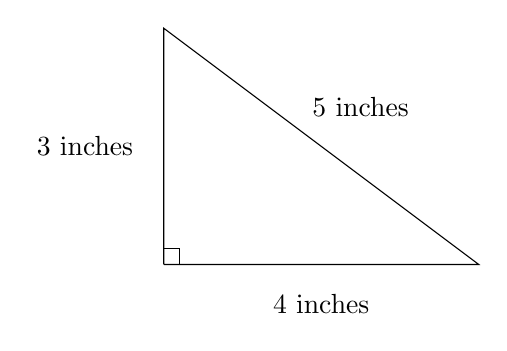
\begin{tikzpicture}
	\draw (0,0) -- (4,0) -- (0,3) -- (0,0);
	\draw (0,0.2) -- (0.2,0.2) -- (0.2,0);
	\draw(2,-0.5) node{$4$ inches};
	\draw(-1,1.5) node{$3$ inches};
	\draw(2.5,2) node{$5$ inches};
\end{tikzpicture}
\captionof{figure}{a triangle}
\label{fig: triPerimeter}
\end{center}

This triangle's perimeter is:
\[ \text{triangle perimeter} = 3+4+5 = 12 \text{ in} \]

\subsection{Rectangle Area}
Earlier, we learned how to find a figure's perimeter---it's the distance around the edge of the figure. Area is a different concept. Let's look at a rectangle cut into small "unit squares." Each unit square's base is $1$ unit in length.

\begin{tightcenter}
   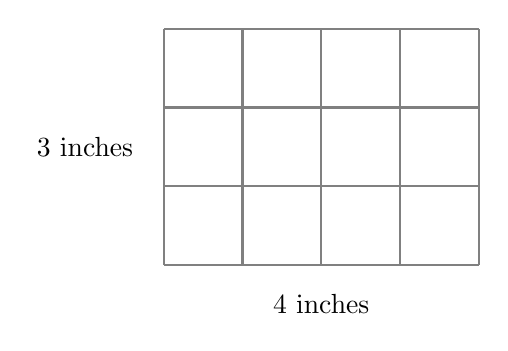
\begin{tikzpicture}
      \draw[step=1.0cm,gray,thick]
      (0,0) grid (4,3);
	\draw(2,-0.5) node{$4$ inches};
	\draw(-1,1.5) node{$3$ inches};
   \end{tikzpicture}
   \captionof{figure}{a $4$-inch-by-$3$-inch rectangle}
   \label{fig: recSquare}
\end{tightcenter}

Each $1$-inch-by-$1$-inch unit square has an area of $1$ square inch. This rectangle has a total of $4 \cdot 3 = 12$ such unit squares, so the rectangle's area is $12$ square inches.

The formula of a rectangle's area is:
\[ \text{rectangle area}=\text{base} \cdot \text{height} \]
or
\[ \text{rectangle area}=\text{length} \cdot \text{width} \]

Note that the unit of this rectangle is "square inch". This is different from the unit of a rectangle's perimeter---inch. The word "square" implies we are dealing with area, not length.

Instead of writing the words "square inches", we could also write $\text{in}^{2}$. Don't confuse this with "square of a number". Let's make a comparison:
\begin{itemize}
\item "$3^{2}$" means "three squared", or $3\cdot3=9$.
\item "$3 \text{ in}^{2}$" means "three square inches", the size of three $1$-inch-by-$1$-inch unit squares.
\end{itemize}

\subsection{Square Area}
A square is a special rectangle, so it's area formula is the same as a rectangle's area formula, except a square's base and height always have the same length. Because of this, instead of writing a square's area formula as $\text{base} \cdot \text{base}$, we can write a square's area formula as

\[ \text{square area} = \text{base}^{2} \]

\begin{myexample}
Find the area of the following square.

\begin{center}
\begin{tikzpicture}
	\draw (0,0) -- (3,0) -- (3,3) -- (0,3) -- (0,0);
	\draw (0,0.2) -- (0.2,0.2) -- (0.2,0);
	\draw(1.5,-0.5) node{$3$ inches};
	\draw(-1,1.5) node{$3$ inches};
	\draw(1.5,3.5) node{$3$ inches};
	\draw(4,1.5) node{$3$ inches};
\end{tikzpicture}
\captionof{figure}{a $3$-inch-by-$3$-inch square}
\label{fig: squArea}
\end{center}
\end{myexample}

\begin{solution}
To find the square's area, we simply do:
\[ \text{square area}=\text{base}^{2}=3^{2}=9 \text{ in}^{2} \]
\end{solution}

\subsection{Triangle Area}
In the following figure, we can clearly see a triangle is half as big as a rectangle with the same base and height.

\pagebreak
\begin{center}
\begin{tikzpicture}
	\draw (0,0) -- (4,0) -- (0,3) -- (0,0);
	\draw (0,0.2) -- (0.2,0.2) -- (0.2,0);
	\draw[dotted] (0,3) -- (4,3) -- (4,0);
	\draw(2,-0.5) node{$4$ in};
	\draw(-0.5,1.5) node{$3$ in};
\end{tikzpicture}
\captionof{figure}{A triangle is half as big as a rectangle.}
\label{fig: triArea1}
\end{center}

To find the area of a triangle, we first find the rectangle's area by $(\text{base})\cdot(\text{height})$, and then divide the rectangle's area by $2$:
\[ \text{triangle area}=\text{base} \cdot \text{height} \div2 \]

The triangle's area in \cref{fig: triArea1} is:
\[ \text{triangle area}=4\cdot3\div2 = 6 \text{ in}^{2} \]

In \cref{fig: triArea1}, the triangle has a right angle ($90$ degrees). It is called a \textit{right triangle}. The same area formula works for non-right triangles.

\begin{center}
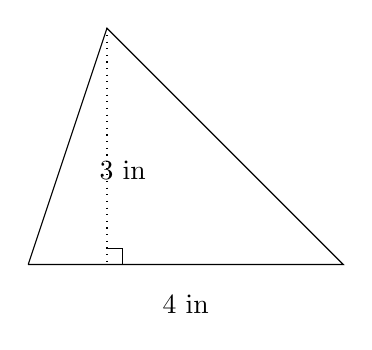
\begin{tikzpicture}
	\draw (0,0) -- (4,0) -- (1,3) -- (0,0);
	\draw[dotted] (1,3) -- (1,0);
	\draw (1.2,0) -- (1.2,0.2) -- (1,0.2);
	\draw(2,-0.5) node{$4$ in};
	\draw(1.2,1.2) node{$3$ in};
\end{tikzpicture}
\captionof{figure}{a non-right triangle}
\label{fig: triArea2}
\end{center}

The triangle's area in \cref{fig: triArea2} is still:
\[ 
\begin{aligned}[t]
	&\phantom{{}=}\text{triangle area} \\
	&= \text{base} \cdot \text{height} \div2 \\
	&=4\cdot3\div2 \\
	&=12\div2 \\
	&=6 \text{ in}^{2} 
\end{aligned}
\]

In \cref{fig: triArea2}, the dotted line is the triangle's \textit{height}. The small square at the bottom of the height implies $90$ degrees. A triangle's height must form a $90$-degree angle with the base.

\subsection{Summary}
Let's review important formulas we learned in this lesson:

\begin{itemize}
\item $\text{rectangle perimeter} = 2(\text{base}+\text{height})$
\item $\text{square perimeter} = 4 \cdot \text{base}$
\item $\text{rectangle area}=\text{base} \cdot \text{height}$
\item $\text{square area}=\text{base}^{2} $
\item $\text{triangle area}=\text{base} \cdot \text{height} \div2$
\end{itemize}



\section{Divisibility Test}

Number sense is critical in the study of mathematics. The first step of building number sense is to memorize the multiplication table. In this lesson, we will learn how to tell whether a number goes into another evenly. For example, without doing division, we know $2$ goes into $126$ evenly (meaning $\frac{126}{2}$ doesn't have remainder). This lesson is also important in building number sense.

\subsection{Divisibility of $2$}
Let's look at the first few multiples of $2$:
\[ 2, 4, 6, 8, 10, 12, 14, 16, 18, 20, 22, 24, ... \]

We can see they are all even numbers, so $2$ goes into all even numbers evenly. In other words, $2$ goes into a number evenly if its last digit is $0,2,4,6 \text{ or } 8$.

\subsection{Divisibility of $10$}
Let's look at some multiples of $10$:
\[ 10, 20, 30, 40, 50, ..., 100, 110, ..., 1230, 1240, ... \]

It's easy to see that $10$ goes evenly into all numbers whose last digit is $0$.

\subsection{Divisibility of $5$}
Let's look at some multiples of $5$:
\[ 5, 10, 15, 20, 25, 30, ..., 100, 105, 110, ..., 1230, 1235, ... \]

It's easy to see that $5$ goes evenly into all numbers whose last digit is $0$ or $5$.

\subsection{Divisibility of $3$ and $9$}
Let's look at some multiples of $3$:
\[ 3,6,9,12,15,...,99,102,105,...,300,303,306,309,312,...3333,3336,3339,3342,... \]

Let's add up all digits of some of these numbers:
\[
\begin{aligned}[t]
   &15:\: 1+5=6 \\
   &102:\: 1+0+2=3 \\
   &309:\:3+0+9=12 \\
   &3342:\: 3+3+4+2=15
\end{aligned}
\]

Notice that $3$ goes evenly into all these sums: $6,3,12,15$.

To judge whether $3$ goes into a number evenly, we add up all digits of this number. If $3$ goes into the sum evenly, $3$ goes into the number evenly.

\begin{myexample}
Does $3$ go into $195$ and $1984$ evenly?
\end{myexample}
\begin{solution}
We add up all digits of $195$, and we have $1+9+5=15$. Since $3$ goes into $15$ evenly, $3$ must go into $195$ evenly. We can use a calculator to verify this: $\frac{195}{3}=65$.

We add up all digits of $1984$, and we have $1+9+8+4=22$. Since $3$ does not go into $22$ evenly, $3$ does not go into $1994$ evenly. We can use a calculator to verify this: $\frac{1984}{3}=661.333...$.
\end{solution}

This rule also works for $9$, but doesn't work for any other numbers.

\begin{myexample}
Does $9$ go into $396$ and $987$ evenly?
\end{myexample}
\begin{solution}
We add up all digits of $396$, and we have $3+9+6=18$. Since $9$ goes into $18$ evenly, $9$ must go into $396$ evenly. We can use a calculator to verify this: $\frac{396}{9}=44$.

We add up all digits of $987$, and we have $9+8+7=24$. Since $9$ does not go into $24$ evenly, $9$ does not go into $987$ evenly. We can use a calculator to verify this: $\frac{987}{9}=109.666...$.
\end{solution}

Again, don't try to use this rule for $4$, $5$, or any number other than $3$ and $9$. Next, let's review all divisibility rules we learned.

\begin{myexample}
Decide whether $2$, $3$, $5$, $9$ and $10$ go into $12,345$ evenly.
\end{myexample}
\begin{solution}
\begin{itemize}
\item Since $12,345$ is odd, $2$ does not go into $12,345$ evenly.
\item Add up all digits of $12,345$, we have $1+2+3+4+5=15$. Since $3$ goes into $15$ evenly, $3$ must go into $12,345$ evenly.
\item Since the last digit of $12,345$ is $5$, $5$ must go into $12,345$ evenly.
\item Add up all digits of $12,345$, we have $1+2+3+4+5=15$. Since $9$ does not go into $15$ evenly, $9$ does not go into $12,345$ evenly.
\item Since the last digit of $12,345$ is $5$, $10$ does not go into $12,345$ evenly.
\end{itemize}
\end{solution}

\begin{myexample}
Decide whether $2$, $3$, $5$, $9$ and $10$ go into $65,430$.
\end{myexample}
\begin{solution}
\begin{itemize}
\item Since $65,430$ is even, $2$ goes into $65,430$ evenly.
\item Add up all digits of $65,430$, we have $6+5+4+3+0=18$. Since $3$ goes into $18$ evenly, $3$ must go into $65,430$ evenly.
\item Since the last digit of $65,430$ is $0$, $5$ must go into $65,430$ evenly.
\item Add up all digits of $65,430$, we have $6+5+4+3+0=18$. Since $9$ goes into $18$ evenly, $9$ goes into $65,430$ evenly.
\item Since the last digit of $65,430$ is $0$, $10$ goes into $65,430$ evenly.
\end{itemize}
\end{solution}

\subsection{Summary}
Let's review important concepts in this lesson.
\begin{itemize}
\item $2$ goes into all even numbers (ending with $0,2,4,6 \text{ or} 8$).
\item If $3$ goes evenly into the sum of all digits of a number, $3$ goes into the number evenly.
\item $5$ goes evenly into all numbers whose last digit is $5$ or $10$.
\item If $9$ goes evenly into the sum of all digits of a number, $9$ goes into the number evenly.
\item $10$ goes evenly into all numbers whose last digit is $10$.
\end{itemize}

Granted, if the question is: "Can $3$ go into $123$ evenly?", you could use the calculator to do the division $123\div3$ and see whether the quotient is an integer or decimal. However, the content of this lesson is very important in building your number sense, which is very important in later mathematics study.



\section{Prime Number}

Prime numbers are the backbone of all numbers. In this lesson, we will learn prime numbers and how to prime factor a number.

\subsection{Factor and Prime}
Since $\frac{8}{2}=4$, we say $2$ is a factor of $8$, because $2$ goes into $8$ four times with no remainder.

Let's look at factors of the first few numbers, starting with $2$:
\begin{itemize}
\item $2$ has two factors: $1$ and $2$.
\item $3$ has two factors: $1$ and $3$.
\item $4$ has three factors: $1,2$ and $4$.
\item $5$ has two factors: $1$ and $5$.
\item $6$ has four factors: $1,2,3$ and $6$.
...
\end{itemize}
We can see a number (except $1$) has at least two factors: $1$ and the number itself.

If a number has only two factors, $1$ and the number itself, this number is a \textit{prime number}. For example, $2$, $3$ and $5$ are prime numbers.

If a number has more than two factors, this number is a \textit{composite number}. For example, $4$ and $6$ are composite numbers.

If a number is an even number bigger than $2$, it has at least $3$ factors: $1$, $2$ and itself. All even numbers, except $2$, are composite numbers.

It's useful to memorize the first few prime numbers, which will be used frequently later: $2,3,5,7,11,13,...$

Note that $1$ is neither a prime number nor a composite number.

\begin{myexample}
Is $245$ prime or composite?
\end{myexample}
\begin{solution}
When we judge whether a number is prime or composite, we look at the first few prime numbers, $2,3,5,7,11,13,...$, and see whether any of them goes into the number evenly.

\begin{itemize}
\item $2$ doesn't go into $245$ evenly, because $245$ is odd.
\item $3$ doesn't go into $245$ evenly, because $3$ doesn't go evenly into $2+4+5=11$.
\item $5$ goes into $245$ evenly, because the last digit of $245$ is $5$.
\end{itemize}
We can tell $245$ is composite because $5$ goes into $245$ evenly, implying $245$ has at least $3$ factors: $1$, $5$ and $245$.
\end{solution}

\begin{myexample}
Is $199$ prime or composite?
\end{myexample}
\begin{solution}
When we judge whether a number is prime or composite, we look at the first few prime numbers, $2,3,5,7,11,13,...$, and see whether any of them goes into the number evenly.

\begin{itemize}
\item $2$ doesn't go into $199$ evenly, because $199$ is odd.
\item $3$ doesn't go into $199$ evenly, because $3$ doesn't go evenly into $1+9+9=19$.
\item $5$ doesn't go into $199$ evenly, because the last digit of $199$ is not $0$ or $5$.
\item To judge whether $7$ goes into $199$ evenly, it's reasonable to use a calculator. We can see $\frac{199}{7}=28.42\hdots$, so $7$ doesn't go into $199$ evenly.
\item With the help of calculator, we can tell neither $11$ nor $13$ goes into $199$ evenly. 
\end{itemize}

Theoretically, we must test all prime numbers smaller than $199$: $17,19,23,...$. In reality, no reasonable instructor would ask you to spend so much time to judge whether a number if prime or composite. After you test $2,3,5,7$ and $11$, and if none of them goes into the number evenly, it's reasonable to say the number is prime.

For this example, $199$ is indeed a prime number.
\end{solution}

\subsection{Prime Factoring}
Prime numbers are backbones of numbers. Each composite number can be written as the product of prime numbers. For example, $15=3\cdot5$ and $12=2\cdot2\cdot3$. The last equation can be re-written in a simpler way as $12=2^{2}\cdot3$. We will learn how to prime factor numbers.

\begin{myexample}
Prime factor $12$.
\end{myexample}
\begin{solution}
First, write down the first few prime numbers: $2,3,5,7,11$. Rarely would an instructor expect you to use bigger prime numbers in prime factoring. We will prime factor $12$ as an example.

To prime factor the number $12$, we look at the first prime number, $2$, and see whether $2$ goes into $12$. It does! We have $12=2\cdot6$.

In $2\cdot6$, the number $2$ is prime, and we cannot further break it down; the number $6$ is not prime, and can be further factored.

Again, we go back to the list of prime numbers, and see whether the first prime number $2$ goes into $6$. It does! Now we have $12=2\cdot6=2\cdot2\cdot3$. We can stop here because all numbers in the product $2\cdot2\cdot3$ are prime numbers.

We can re-write the product with exponent: $12=2^{2}\cdot3$.

It's easier to use a tree to prime factor numbers:
\[
\begin{forest}
   [12
      [2]
      [6
         [2]
         [3]
      ]
   ]
\end{forest}
\]
\end{solution}

Note that we don't use the number $1$ in prime factoring. Otherwise, we could keep going with no end like $12=2^{2}\cdot3\cdot1\cdot1\cdot...$.

\begin{myexample}
Prime factor 250.
\end{myexample}
\begin{solution}
We will use a factor tree to solve this problem.
\[
\begin{forest}
   [250
      [2]
      [125
         [5]
         [25
            [5]
            [5]
         ]
      ]
   ]
\end{forest}
\]
The prime factor of $250$ is $250=2\cdot5^{3}$.
\end{solution}

We can see a big number like $250$ can be broken down to the product of very small prime numbers.


\section{Greatest Common Factor and Least Common Multiple}

In this lesson, we learn how to find the GCF (Greatest Common Factor) and LCM (Least Common Multiple) of a group of numbers (usually two numbers).

For example, the GCF of $6$ and $8$ is $2$. The LCM of $6$ and $8$ is $24$. These two concepts will help you better understand numbers. In later lessons, we need to find LCM of denominators when we add or subtract fractions.

\subsection{GCF (Greatest Common Factor)}
We will find the GCF of $12$ and $18$. We will list both numbers' factors:

\begin{itemize}
\item Factors of $12$ are: $1,2,3,4,6,12$.
\item Factors of $18$ are: $1,2,3,6,9,18$.
\end{itemize}

The \textit{common} factors of $12$ and $18$ are: $1,2,3,6$.

The GCF (Greatest Common Factor) of $12$ and $18$ is $6$.

Note that we listed all factors of $12$ and $18$ in order to find their GCF. There is an easier method. We will prime factor both numbers:
\[
\begin{tabular}{ l c r }
  \begin{forest} [12[2][6[2][3]]]\end{forest} &  & \begin{forest} [18[2][9[3][3]]]\end{forest} \\
\end{tabular}
\]
We have:
\[
\begin{aligned}[t]
&12=2\cdot2\cdot3 \\
&18=2\cdot3\cdot3
\end{aligned}
\]

Since $12$ and $18$ share the following factors, one $2$ and one $3$, the GCF of $12$ and $18$ is $2\cdot3=6$.

Let's look at another example.

\begin{myexample}
Find the GCF of $24$ and $36$.
\end{myexample}
\begin{solution}
We will prime factor both $24$ and $36$:
\[
\begin{tabular}{ l c r }
  \begin{forest} [24[2][12[2][6[2][3]]]]\end{forest} &  & \begin{forest} [36[2][18[2][9[3][3]]]]\end{forest} \\
\end{tabular}
\]
We have:
\[
\begin{aligned}[t]
&24=2\cdot2\cdot2\cdot3 \\
&36=2\cdot2\cdot3\cdot3
\end{aligned}
\]
We can see $24$ and $36$ share the following factors, two $2$'s and one $3$, so the GCF of $24$ and $36$ is $2\cdot2\cdot3=12$.
\end{solution}

\begin{myexample}
Find the GCF of $8$ and $15$.
\end{myexample}
\begin{solution}
Prime factor both numbers, we have:
\[
\begin{aligned}[t]
&8=2\cdot2\cdot2 \\
&15=3\cdot5
\end{aligned}
\]
We can see $8$ and $15$ don't share any factors. The GCF of $8$ and $15$ is $1$, because $1$ is a factor of all natural numbers.
\end{solution}

\begin{myexample}
Find the GCF of $5$ and $7$.
\end{myexample}
\begin{solution}
Both $5$ and $7$ are prime numbers, so it's impossible for them to share any factor except $1$. So $1$ is the GCF of $5$ and $7$.
\end{solution}

\begin{myexample}
Find the GCF of $10$ and $20$.
\end{myexample}
\begin{solution}
Since $10$ goes into $20$ evenly, the GCF of $10$ and $20$ is simply $10$, because $10$ goes into both $10$ and $20$ evenly.
\end{solution}

\subsection{LCM (Least Common Multiple)}
We will find the LCM of $6$ and $8$. First, we will find the first few multiples of $6$ and $8$:
\begin{itemize}
\item The first few multiples of $6$ are: $6,12,18,24,30,36,42,48,54,...$.
\item The first few multiples of $8$ are: $8,16,24,32,40,48,56...$.
\end{itemize}

We can see $6$ and $8$ have some \textit{common} multiples: $24,48,...$. The \textit{least} common multiple is $24$.

Later, when we do $\frac{1}{6}+\frac{1}{8}$, we need to change the denominator of both fractions to $24$, the LCM of $6$ and $8$. We will learn details later, but here is the solution:
\[
\begin{aligned}[t]
   &\phantom{{}=}\frac{1}{6}+\frac{1}{8} \\
   &= \frac{1\cdot4}{6\cdot4}+\frac{1\cdot3}{8\cdot3} \\
   &= \frac{4}{24}+\frac{3}{24} \\
   &= \frac{4+3}{24} \\
   &= \frac{7}{24}
\end{aligned}
\]

As an example, we will find the LCM of $6$ and $8$ in two methods.
\subsubsection{Method 1 to Find LCM}
We will prime factor both $6$ and $8$:
\[
\begin{aligned}[t]
&6=2\cdot3 \\
&8=2\cdot2\cdot2
\end{aligned}
\]

The LCM of $6$ and $8$ must \textit{cover} the prime factors of both numbers:
\begin{itemize}
\item The LCM of $6$ and $8$ must have three $2$'s as factors, as $6$ needs one $2$ and $8$ needs three $2$'s.
\item The LCM of $6$ and $8$ must have one $3$ as a factor, as $6$ needs one $3$.
\end{itemize}
Putting them together, the LCM must have three $2$'s and one $3$ as factors. We have: $\text{LCM}=2\cdot2\cdot2\cdot3=24$.

To verify, we have $\frac{24}{6}=4$, and $\frac{24}{8}=3$.

\subsubsection{Method 2 to Find LCM}
List the first few multiples of the \textit{bigger} number until the smaller number goes into a multiple evenly:

The first few multiples of $8$ are: $8,16,24$.

We stopped here because $6$ goes into $24$ evenly, so $24$ is the LCM of $6$ and $8$. To verify, we have $\frac{24}{6}=4$, and $\frac{24}{8}=3$.

Which method should we use? Most of the time, the second method is faster, so try the second method first. Sometimes the first method is faster.

\begin{myexample}
Find the LCM of $4$ and $12$.
\end{myexample}
\begin{solution}
Since $4$ goes into $12$, the LCM of $4$ and $12$ is simply $12$.

To verify, we have $\frac{12}{4}=3$ and $\frac{12}{12}=1$.
\end{solution}

\begin{myexample}
Find the LCM of $8$ and $18$.
\end{myexample}
\begin{solution}
We list the first few multiples of $18$, until $8$ goes evenly into one of them:

Multiples of $18$: $18$,$36$,$54$,$72$.

We stop here because $\frac{72}{8}=9$. The LCM of $8$ and $18$ is $72$.

To verify, we have $\frac{72}{8}=9$ and $\frac{72}{18}=4$.
\end{solution}

\begin{myexample}
Find the LCM of $24$ and $28$.
\end{myexample}
\begin{solution}
We list the first few multiples of $28$, until $24$ goes evenly into one of them:

Multiples of $28$: $28$,$56$,$84$,$112$,$140$...

$24$ doesn't go evenly into any of them. After listing $5$ multiples, we know this method is not the best method to find the LCM. We will try the other method. We will prime factor both numbers:
\[
\begin{tabular}{ l c r }
  \begin{forest} [28[2][14[2][7]]]\end{forest} &  & \begin{forest} [24[2][12[2][6[2][3]]]]\end{forest} \\
\end{tabular}
\]
We have:
\[
\begin{aligned}[t]
&28=2\cdot2\cdot7 \\
&24=2\cdot2\cdot2\cdot3
\end{aligned}
\]
The LCM of $28$ and $24$ must \textit{cover} the prime factors of both numbers:
\begin{itemize}
\item The LCM must have three $2$'s as factors, as $24$ needs three $2$'s and $28$ needs two $2$'s.
\item The LCM must have one $3$ as a factor, as $24$ needs one $3$.
\item The LCM must have one $7$ as a factor, as $28$ needs one $7$.
\end{itemize}
Putting them together, the LCM must have three $2$'s, one $3$ and one $7$ as factors. We have: $\text{LCM}=2\cdot2\cdot2\cdot3\cdot7=168$.

To verify, we have $\frac{168}{28}=6$, and $\frac{168}{24}=7$.
\end{solution}


\section{Order of Operations}

In this lesson, we will learn the order of operations -- Parentheses, Exponent, Multiplication, Division, Addition, Subtraction.

\subsection{MD and AS}

Most likely, you remember from middle school the acronym PEMDAS (Please Excuse My Dear Aunt Sally). In order of operations, we should follow the order Parentheses, Exponent, Multiplication, Division, Addition, Subtraction. There is a better way to write this acronym:

\[
\begin{aligned}[t]
   &P &\text{(Parentheses)} \\
   &E &\text{(Exponent)} \\
   &MD &\text{(Multiplication and Division)} \\
   &AS &\text{(Addition and Subtraction)}
\end{aligned}
\]
\captionof{figure}{Order of Operations}
\label{fig:PEMDAS18}

What's the difference? If we simply write PEMDAS, we could wrongly assume that multiplication overrides division, and that addition overrides subtraction. This is not true.

Addition and subtraction are at the same level of order of operations. They cannot override each other. We do the operation which comes first (on the left). Compare the following two examples:

\begin{myexample}
\begin{tabular}[t]{c@{\hspace{4cm}}c@{\hspace{2cm}}c}
&
$ \begin{aligned}[t] &\phantom{{}=} \underline{4+3}-1 \\ &= 7 \phantom{+3} -1 \\ &= 6 \end{aligned} $ 
&
$ \begin{aligned}[t] &\phantom{{}=} \underline{4-3}+1 \\ &= 1 \phantom{-3} +1 \\ &= 2 \end{aligned} $
\end{tabular}
\end{myexample}

It's a good practice to underline the next step, like in the examples above. Note the problem will not come with underlines. You have add them in yourself.

In the example on the right side, we did subtraction first because subtraction came first (on the left). Addition cannot override subtraction, because they are at the same level in the order of operations. This is why we should not write PEMDAS horizontally, and should instead write it vertically as in \cref{fig:PEMDAS18}.

Similarly, multiplication and division cannot override each other. Look at the next two examples.

%\begin{myexample}
% $ 
%\begin{aligned}[t] 
%\underline{12\cdot3}\div4 &= 36 \phantom{11} & \underline{12\cdot3}\div4 &= 36 \phantom{11} \\ 
%&= 9  &= 9  
%\end{aligned} $ 
%\end{myexample}

\begin{myexample}	
\begin{tabular}[t]{c@{\hspace{4cm}}c@{\hspace{2cm}}c}
&
 $ 
\begin{aligned}[t] 
   &\phantom{{}=} \underline{12\cdot3}\div4 \\
   &= 36 \phantom{11} \div 4\\ 
   &= 9  
\end{aligned} $ 
&
 $ 
\begin{aligned}[t] 
   &\phantom{{}=} \underline{12\div3}\cdot4 \\
   &= 4 \phantom{|111} \cdot 4\\ 
   &= 16  
\end{aligned} $ 
\end{tabular}
\end{myexample}

In the example on the right side, we did division first because it came before multiplication.

\subsection{Basic Order of Operations}


The next few examples show how to follow the order of operations as in  \cref{fig:PEMDAS18}.

\begin{myexample}
\[
\begin{aligned}[t]
    &\phantom{{}=} 10-\underline{2\cdot3}    \\
    &= 10-6 \\
   &= 4
\end{aligned}
\]

In the example above, multiplication overrides subtraction, so we did $2\cdot3$ first.
\end{myexample}

\begin{myexample}
\[
\begin{aligned}[t]
   &\phantom{{}=} \underline{(10-2)}\cdot3 \\
   &= 8\cdot3 \\
   &= 24
\end{aligned}
\]
In the example above, parentheses override multiplication, so we did $10-2$ first.
\end{myexample}

\begin{myexample}
\[
\begin{aligned}[t]
   &\phantom{{}=} 3\cdot \underline{2^{3}} \\
   &= 3\cdot 8 \\
   &= 24
\end{aligned}
\]
In the example above, exponent overrides multiplication, so we did $2^{3}$ first. Note that $2^{3}=2\cdot2\cdot2=4\cdot2=8$. It's a common mistake to do $2^{3}=6$.
\end{myexample}

\begin{myexample}
\[
\begin{aligned}[t]
   &\phantom{{}=} \underline{(3\cdot2)}^{3} \\
   &= 6^{3} \\
   &= 6\cdot6\cdot6 \\
   &= 216
\end{aligned}
\]
In the example above, parentheses override exponent, so we did $3\cdot2$ first.
\end{myexample}


\subsection{Implied Multiplication}

Earlier, we learned that we don't use the multiplication symbol any more. We use a dot instead. For example, instead of writing $2\times3=6$, we write $2\cdot3=6$.

Mathematicians decide to write less whenever possible. Sometimes, even the dot can be omitted. For example, instead of writing $2\cdot(3+4)$, we write $2(3+4)$.

So, in many situations, if there is no operation symbol ($+,-,\cdot,\div$), it implies multiplication. For example:

\[
\begin{aligned}[t]
   & 2(3)=2\cdot3=6 \\
   & 2x \text{ implies } 2\cdot x \\
   & 2(3-1)=2\cdot2=4
\end{aligned}
\]

Note that if you want to write $2\cdot3$, you have to write the multiplication symbol (the dot). Otherwise it becomes twenty-three. So, you can only omit the multiplication symbol when there won't be any confusions.

\begin{myexample}
\[
\begin{aligned}[t]
   &\phantom{{}=} \underline{(7-2)}4 \\
   &= (5)4 \\
   &= 20
\end{aligned}
\]
In the example above, there is no operation symbol between $(7-2)$ and $4$, which implies multiplication.

Since parentheses override multiplication, we did $(7-2)$ first.
\end{myexample}


\subsection{Multi-Step Examples}

In this section, we will tackle some complicated order of operations problems. The key is to underline the next step, and do the problem step by step. As a beginner, don't try to do two steps at once.

\begin{myexample}
\[
\begin{aligned}[t]
   &\phantom{{}=} \underline{(7-2)}^{2}+3(7-2^{2}) \\
   &= 5^{2}+3(7-\underline{2^{2}}) &\text{There is no need to write }(5)^{2}\\
   &= 5^{2}+3\underline{(7-4)} \\
   &= \underline{5^{2}}+3(3) &\text{We could write }3\cdot3\\
   &= 25+\underline{3(3)} \\
   &= 25+9 \\
   &= 34
\end{aligned}
\]
Once we complete all operations inside a pair of parentheses, the parentheses have done the job, and we can omit them. For example, in the second step of this example, we could write $(5)^{2}$, or $5^{2}$. It's your choice.
\end{myexample}

When there are parentheses inside parentheses, we use brackets, "[ ]", as the outside parentheses to differentiate those two pairs of parentheses. We need to take care of the inside pair first.

\begin{myexample}
\[
\begin{aligned}[t]
   &\phantom{{}=}23-2[3^{2}-\underline{(4-3)}] \\
   &= 23-2[\underline{3^{2}}-1] \\
   &= 23-2\underline{[9-1]} \\
   &= 23-\underline{2[8]} &\text{Don't do subtraction first!} \\
   &= 23-16 \\
   &= 7
\end{aligned}
\]

In the step $23-2[8]$, note that there is no operation symbol between $2$ and $[8]$, which implies multiplication. Multiplication overrides subtraction, so we need to do $2\cdot[8]$ first.

We could re-write $2[8]$ as $2\cdot8$. Since only one number, $8$, remains in the parentheses, we can omit the parentheses. However, we do need to add a multiplication symbol. Otherwise $2[8]$ would become $28$.
\end{myexample}
\bigskip

\subsection{Fraction Line}
\bigskip

Earlier, we learned that the fraction line means division. We will learn how to do order of operations problems involving fraction line.

Compare these two examples:

\begin{myexample}
\begin{tabular}[t]{c@{\hspace{4cm}}c@{\hspace{2cm}}c}
&
 $ \begin{aligned}[t] &\phantom{{}=} 6+\frac{4}{2} \\ &= 6 +2 \\ &= 8 \end{aligned} $ & $ \begin{aligned}[t] &\phantom{{}=} \frac{6+4}{2} \\ &= \frac{10}{2} \\ &= 5 \end{aligned} $ \\
\end{tabular}
\end{myexample}

On the left side, we need to do division before addition.

On the right side, we have to do addition before division. We could imagine a pair of "invisible" parentheses in both the numerator and denominator of a fraction, like:
\[ \frac{6+4}{2}=\frac{(6+4)}{(2)} \]

Let's look at a more complicated example.

\begin{myexample}
\[
\begin{aligned}[t]
   &\phantom{{}=} \frac{28-2(3)}{6^{2}-5^{2}} \\
   &= \frac{28-2(3)}{36-5^{2}} \\
   &= \frac{28-2(3)}{36-25} \\
   &= \frac{28-6}{36-25} \\
   &= \frac{22}{36-25} \\
   &= \frac{22}{11} \\
   &= 2
\end{aligned}
\]
When a fraction line is involved, we evaluate the numerator first, then the denominator, and finally do the division.
\end{myexample}



\chapter{Integer Operations}
\thispagestyle{fancy}
\section{Number Line and Absolute Value}

In this lesson, we will learn the concept of negative numbers, and their positions on the number line. We will also learn the concept of absolute value.

\subsection{Positive and Negative Numbers}

Negative numbers are regularly used in every day life. For example:

\begin{itemize}
\item The stock market lost $30.2$ points yesterday.
\item Today's temperature is $10$ degrees below zero.
\item Mr. Smith overdrew his bank account by \$$50$.
\item The wreck of Titanic is $12,420$ feet under water.
\item A company lost \$$2$ million dollars last year.
\end{itemize}

Each of the above situations can be modeled by a negative number. For example, if today's temperature is $10$ degrees below zero, we say the temperature is $-10$ degrees.

We use the word \textit{integers} to represent the set $\{...,-4,-3,-2,-1,0,1,2,3,4,...\}$. We use a number line to visualize numbers. For example, \cref{fig:NumberLine1} shows the integer $-1$ on the number line.

\begin{tightcenter}
	\begin{tikzpicture}
		\begin{axis}[
				xmin=-5,xmax=5,
				ymin=-1,ymax=1,
				axis y line=none,
				height =1cm,
				grid=none,
				xtick={-4,-3,...,4},
				xlabel={},
					]
			\addplot+[soldot]coordinates{ (-1,0) };				
		\end{axis}
	\end{tikzpicture}
	\captionof{figure}{$-1$ on the number line}
	\label{fig:NumberLine1}
\end{tightcenter}

On a number line, the right is the positive direction, and the left is the negative direction. A bigger number is always located to the right side of a smaller number. 

Let's quickly review two inequality symbols:
\begin{itemize}
\item The symbol ">" is read as "greater than". For example, $2>1$ is read as "two is greater than one."
\item The symbol "<" is read as "less than". For example, $1<2$ is read as "one is less than two."
\end{itemize}

Look at the number line in \cref{fig:NumberLine2} with four numbers marked:

\begin{figure}[!htb]
\centering
	\begin{tikzpicture}
		\begin{axis}[
				xmin=-5,xmax=5,
				ymin=-1,ymax=1,
				axis y line=none,
				height =1cm,
				grid=none,
				xtick={-4,-3,...,4},
				xlabel={},
					]
			\addplot+[soldot]coordinates{ (-1,0) };		
			\addplot+[soldot]coordinates{ (-3,0) };	
			\addplot+[soldot]coordinates{ (0,0) };	
			\addplot+[soldot]coordinates{ (2,0) };			
		\end{axis}
	\end{tikzpicture}
	\captionof{figure}{$-3$, $-1$, $0$ and $2$ on the number line}
	\label{fig:NumberLine2}
\end{figure}

We can observe the following relationship:
\begin{itemize}
\item $2>-3$ since $2$ is located to the right of $-3$;
\item $0>-1$ since $0$ is located to the right of $-1$;
\item $-1>-3$ since $-1$ is located to the right of $-3$.
\end{itemize}

Putting together those four numbers, we have $2>0>-1>-3$. Notice that:
\begin{itemize}
\item Positive numbers are bigger than 0 and negative numbers.
\item The number 0 is bigger than negative numbers.
\item Compare $3>1$ and $-1>-3$. This is because, on the number line, $3$ is located to the right of $1$, and $-1$ is located to the right of $-3$.
\end{itemize}

\subsection{Absolute Value}
The absolute value of a number is the distance between the number and $0$ on the number line.

How far is the number $2$ from $0$ on the number line? The distance is obviously two units, so the absolute value of $2$ is simply $2$.

Similarly, the distance between $-2$ and $0$ on the number line is also two units, so the absolute value of $-2$ is $2$.

\begin{figure}[!htb]
\centering
	\begin{tikzpicture}
		\begin{axis}[
				xmin=-5,xmax=5,
				ymin=-1,ymax=2,
				axis y line=none,
				height =1cm,
				grid=none,
				xtick={-4,-3,...,4},
				xlabel={},
					]	
			\addplot+[soldot]coordinates{ (-2,0) };	
			\addplot[<->,line width=3pt,red,domain=-2:0]{0.5} node[pos=0.5,anchor=south]{2};
			\addplot+[soldot,color=blue]coordinates{ (2,0) };	
			\addplot[<->,line width=3pt,blue,domain=0:2]{0.5} node[pos=0.5,anchor=south]{2};
		\end{axis}

	\end{tikzpicture}
	\captionof{figure}{Absolute Value of $2$ and $-2$}
	\label{fig:AbsoluteValue}
\end{figure}

Here is how we write absolute value with its math symbol:
\begin{itemize}
\item The absolute value of $2$ is $2$, written as $\lvert 2 \rvert =2$.
\item The absolute value of $-2$ is $2$, written as $\lvert -2 \rvert=2$.
\end{itemize}

Here are a few examples:

\[
\begin{aligned}[t]
	\lvert 0 \rvert &=0 \\
	\lvert -1 \rvert &=1 \\
	-\lvert 1 \rvert &=-1
\end{aligned}
\]

The absolute value of $0$ is simply $0$, because the distance between $0$ and $0$ on the number line is $0$.

Note the difference between the last two examples. Absolute value can change a negative number to positive, as long as the number is inside the absolute value symbol, as in $\lvert -1 \rvert =1$.

However, absolute value cannot affect the negative symbol outside the absolute value symbol, as in $-\lvert 1 \rvert =-1$.



\section{Add and Subtract Integers}

In this lesson, we will learn how to add and subtract positive and negative integers.

\subsection{Add Integers}
I will show two methods to add integers. You choose the method which makes 
more sense for you. We will calculate $(-1)+(-2)$.
\begin{method}
	\item The first method is the traditional number line method. Recall that the 
right side is the positive direction, and the left side is negative direction.
	\begin{steps}
		\item Locate the first number, $-1$, on the number line.
		\begin{tightcenter}
			\begin{tikzpicture}
				\begin{axis}[
						xmin=-5,xmax=5,
						ymin=-1,ymax=2,
						axis y line=none,
						height =1cm,
						grid=none,
						xtick={-4,-3,...,4},
						xlabel={}
					]
					\addplot+[soldot]coordinates{ (-1,0) };				
				\end{axis}
			\end{tikzpicture}
			\captionof{figure}{Locate $-1$ on the number line}
		\end{tightcenter}
		\item The second number is $-2$, meaning we will move to the \emph{left} (negative direction) by two units.
		\begin{tightcenter}
			\begin{tikzpicture}
				\begin{axis}[
						xmin=-5,xmax=5,
						ymin=-1,ymax=2,
						axis y line=none,
						height =1cm,
						grid=none,
						xtick={-4,-3,...,4},
						xlabel={}
					]
					\addplot[soldot]coordinates{ (-1,0) };	
					\addplot[<-,line width=3pt,red,domain=-3:-1]{0.5} node[pos=0.5,anchor=south]{$-2$};			
				\end{axis}
			\end{tikzpicture}
			\captionof{figure}{From $-1$ move to the left by $2$ units}
		\end{tightcenter}
		\item After the move, we reached the number $-3$ on the number line. This implies that
		\[
			(-1)+(-2)=-3
		\]
	\end{steps}
	\item The second method uses a money model. We deal with money every day, so most students easily understand this method.
	
	\begin{steps}
	\item Say you are gambling. The first number is $-1$, meaning you lost \$1 in the first game. 
	\item The second number is $-2$, meaning you lost \$2 in the second game. 
	\item Since you lost in both games, altogether, you lost. This implies the answer must be negative.
	\item Since you lost in both games, all together, you lost \$1+\$2=\$3.
	\end{steps}
	Finally, we have \[(-1)+(-2)=-3\]
\end{method}

Let's look at a few more examples.

\begin{myexample}
Calculate $4+(-5)$
\end{myexample}
\begin{solution}
	We will use the number line method.
	\begin{steps}
		\item Locate the first number, $4$, on the number line.
		\begin{tightcenter}
			\begin{tikzpicture}
				\begin{axis}[
						xmin=-5,xmax=5,
						ymin=-1,ymax=1,
						axis y line=none,
						height =1cm,
						grid=none,
						xtick={-4,-3,...,4},
						xlabel={}
					]
					\addplot+[soldot]coordinates{ (4,0) };				
				\end{axis}
			\end{tikzpicture}
			\captionof{figure}{Locate $4$ on the number line}
		\end{tightcenter}
		\item The second number is $-5$, meaning we will move to the \emph{left} (negative direction) by five units.
		\begin{tightcenter}
			\begin{tikzpicture}
				\begin{axis}[
						xmin=-5,xmax=5,
						ymin=-1,ymax=2,
						axis y line=none,
						height =1cm,
						grid=none,
						xtick={-4,-3,...,4},
						xlabel={}
					]
					\addplot[<-,line width=3pt,red,domain=-1:4]{0.5} node[pos=0.5,anchor=south]{$-5$};	
					\addplot[soldot]coordinates{ (4,0) };		
				\end{axis}
			\end{tikzpicture}
			\captionof{figure}{From $4$ move to the left by $5$ units}
		\end{tightcenter}
		\item After the move, we reached the number $-1$ on the number line. This implies:
		\[
			4+(-5)=-1
		\]
	\end{steps}
\end{solution}

\begin{myexample}
Calculate $(-4)+5$
\label{ex:e-4+5}
\end{myexample}
\begin{solution}
We will use the money model to solve this problem.
	\begin{steps}
	\item Say you are gambling. The first number is $-4$, meaning you lost \$4 in the first game. 
	\item The second number is $5$, meaning you won \$5 in the second game. 
	\item Since you won more money than you lost, altogether, you won. This implies the answer must be positive.
	\item Since you lost some and then won some, we should find the difference of those two numbers' absolute values: \$$5-$\$$4$=\$$1$.
	\end{steps}
	Finally, we have \[(-4)+5=1\]
\end{solution}

If you are new to negative numbers, the number line method can help you understand integer operations. When numbers are big, it's difficult to locate numbers on the number line; the money model would work better.

\begin{myexample}
Calculate $(-44)+15$
\end{myexample}
\begin{solution}
We will use the money model to solve this problem.
	\begin{steps}
	\item Say you are gambling. The first number is $-44$, meaning you lost \$44 in the first game. 
	\item The second number is $15$, meaning you won \$15 in the second game. 
	\item Since you lost more money than you won, altogether, you lost. This implies the answer must be negative.
	\item Since you lost some and then won some, we should find the difference of those two numbers' absolute values: \$$44-$\$$15$=\$$29$.
	\end{steps}
	Finally, we have \[(-44)+15=-29\]
	Don't forget the negative sign in the answer (because you lost money).
\end{solution}

\subsection{Subtract a Positive Integer}
Let's observe a pattern first:
\begin{align*}
	&3-2 = 1 \longleftrightarrow 3+(-2) =1 \\
	&4-3 =1  \longleftrightarrow 4+(-3) =1 \\
	&1-3 =-2  \longleftrightarrow 1+(-3) =-2 
\end{align*}

We can see the subtraction sign and negative symbol have the same functions! Starting today, it would be great if you can treat the subtraction sign as a negative symbol. When we subtract a positive number, we can treat it as "adding a negative number", and then use the methods we learned earlier to add integers.

\begin{myexample}
Calculate $-4-5$
\end{myexample}
\begin{solution}
First, we change subtraction to "adding a negative":
\[ -4-5=(-4)+(-5) \]
Note that the parentheses around $-4$ is optional, just to make it clear. The parentheses around $-5$ is needed, as it's confusing to write two symbols right next to each other, like $-4+-5$.
Next, we will use the money model to solve this problem.
	\begin{steps}
	\item Say you are gambling. The first number is $-4$, meaning you lost \$4 in the first game. 
	\item The second number is $-5$, meaning you lost \$5 in the second game. 
	\item Since you lost money in both games, altogether, you lost. This implies the answer must be negative.
	\item Since you lost in both games, we should find the sum of those two numbers' absolute values: \$$5+$\$$4$=\$$9$.
	\end{steps}
	Finally, we have \[-4-5=(-4)+(-5)=-9\]
\end{solution}

\begin{myexample}
Calculate $4-5$
\end{myexample}
\begin{solution}
First, we change subtraction to "adding a negative":
\[ 4-5=4+(-5) \]
Next, we will use the money model to solve this problem.
	\begin{steps}
	\item Say you are gambling. The first number is $4$, meaning you won \$4 in the first game. 
	\item The second number is $-5$, meaning you lost \$5 in the second game. 
	\item Since you lost more money than you won, altogether, you lost. This implies the answer must be negative.
	\item Since you won some money and then lost some, we should find the difference of those two numbers' absolute values: \$$5-$\$$4$=\$$1$.
	\end{steps}
	Finally, we have \[4-5=4+(-5)=-1\]
\end{solution}

Don't be silly when you do problems like $9-5$. There is no need to use the number line or money model, as $9-5=4$. :)

\subsection{Subtract a Negative Integer}
Here is the bottom line: When two negative signs are right next to each other, we change these two negative signs to one positive sign, as in
\[ 1-(-2)=1+2 \]

For now, memorize this as a rule. In the next lesson, we will understand why.

Look at the difference between these two problems:
\[
\begin{aligned}[t]
   &\phantom{{}=}1-(-2) &\phantom{aaaaaaaaaaaaaaaaaaa}& \phantom{{}=}-1-2 \\
   &=1+2 &\phantom{aaaaaaaaaaaaaaaaaaa} & =-3 \\
   &=3
\end{aligned}
\]

We only change two negative signs to one positive sign if they are right next to each other. In $-1-2$, a number separated those two negative signs, so we cannot change them to one positive sign.

\begin{myexample}
Calculate $-4-(-5)$
\end{myexample}
\begin{solution}
	First, we change two negative signs to one positive sign:
	\[ -4-(-5)=-4+5 \]
	The rest of the solution is the same as in \cref{ex:e-4+5}.
	Finally, we have \[-4-(-5)=-4+5=1\]
\end{solution}

Finally, let's look at an example to put together what we learned in this lesson.

\begin{myexample}
Calculate $-3-(-5)-(-9)-14$
\begin{solution}
	The first step is to change two negative signs (right next to each other) to one positive sign:
		\[
		\begin{aligned}[t]
			&\phantom{{}=} -3-(-5)-(-9)-14 \\
			& = -3+5+9-14 \\
		\end{aligned}
		\]
	Next, we use either the number line model or money model to do additions and subtractions step by step. The full solution is:
		\[
		\begin{aligned}[t]
			&\phantom{{}=} -3-(-5)-(-9)-14 \\
			& = -3+5+9-14 \\
            & = 2+9-14     \\
            & = 11-14 \\
            &= -3
		\end{aligned}
		\]
\end{solution}
\end{myexample}




\section{Multiply and Divide Integers}
\thispagestyle{fancy}
In this lesson, we will learn how to multiply and divide positive and negative integers.

\subsection{Multiply Integers}
Assume you are walking on a number line. Remember a number line has a positive direction and a negative direction. Assume you are facing the positive direction.

If you walk backward at a speed of $2$ feet per step, you would walk in the negative direction. We can say you walk $-2$ feet per step.

In $3$ steps, you would walk $6$ feet in the negative direction. We could do

\[ (-2)+(-2)+(-2)=-6 \]

Easier, we can use multiplication:

\[ (-2)\cdot3=-6 \]

We can see this in the figure:

		\begin{tightcenter}
			\begin{tikzpicture}
				\begin{axis}[
						xmin=-8,xmax=8,
						ymin=-1,ymax=2,
						axis y line=none,
						height =1cm,
						grid=none,
						xtick={-7,-6,...,7},
						xlabel={}
					]
					\addplot[<-,line width=3pt,red,domain=-2:0]{0.5} node[pos=0.5,anchor=south]{$-2$};
					\addplot[<-,line width=3pt,red,domain=-4:-2]{0.5} node[pos=0.5,anchor=south]{$-2$};
					\addplot[<-,line width=3pt,red,domain=-6:-4]{0.5} node[pos=0.5,anchor=south]{$-2$};	
					\addplot[soldot]coordinates{ (0,0) };			
					\addplot[soldot]coordinates{ (-2,0) };
					\addplot[soldot]coordinates{ (-4,0) };
					\addplot[soldot]coordinates{ (-6,0) };
				\end{axis}
			\end{tikzpicture}
			\captionof{figure}{$(-2)\cdot3=-6$}
		\end{tightcenter}

We can see:
\[ \text{(negative)}\cdot\text{(positive)}=\text{negative} \]

The next rule is:
\[ \text{(negative)}\cdot\text{(negative)}=\text{positive} \]

There are two ways to understand this.

An easy way is to think about this sentence: I do NOT NOT like football. Since double-negation implies affirmation, this sentence actually means "I do like football." This is why $ \text{(negative)}\cdot\text{(negative)}=\text{positive} $.

Another way is to use the number line. In $(-2)\cdot(-3)$, the number $-2$ implies a person walks \textit{backward} $2$ feet per step; the number $-3$ implies this person walks $3$ steps while \textit{facing the negative direction}. In this situation, since the person faces the negative direction while walking backward, the person is actually moving \textit{in the positive direction}! See the following figure:

		\begin{tightcenter}
			\begin{tikzpicture}
				\begin{axis}[
						xmin=-8,xmax=8,
						ymin=-1,ymax=2,
						axis y line=none,
						height =1cm,
						grid=none,
						xtick={-7,-6,...,7},
						xlabel={}
					]
					\addplot[->,line width=3pt,red,domain=0:2]{0.5} node[pos=0.5,anchor=south]{$2$};
					\addplot[->,line width=3pt,red,domain=2:4]{0.5} node[pos=0.5,anchor=south]{$2$};
					\addplot[->,line width=3pt,red,domain=4:6]{0.5} node[pos=0.5,anchor=south]{$2$};	
					\addplot[soldot]coordinates{ (0,0) };			
					\addplot[soldot]coordinates{ (2,0) };
					\addplot[soldot]coordinates{ (4,0) };
					\addplot[soldot]coordinates{ (6,0) };
				\end{axis}
			\end{tikzpicture}
			\captionof{figure}{$(-2)\cdot(-3)=6$}
		\end{tightcenter}

Let's summarize multiplication rules:
\[
\begin{aligned}[t]
	&\text{(positive)}\cdot\text{(positive)}=\text{positive}&&\text{example}: 2\cdot3=6\\
	&\text{(negative)}\cdot\text{(positive)}=\text{negative}&&\text{example}: (-2)\cdot3=-6\\
	&\text{(positive)}\cdot\text{(negative)}=\text{negative}&&\text{example}: 2\cdot(-3)=-6\\
	&\text{(negative)}\cdot\text{(negative)}=\text{positive}&&\text{example}: (-2)\cdot(-3)=6\\
\end{aligned}
\]

\begin{myexample}
Calculate $(-1)(-2)(-3)$
\end{myexample}
\begin{solution}
We learned that, in multiplication, $\text{(negative)}\cdot\text{(negative)}=\text{positive}$. In other words, each pair of negative signs cancel each other.

In this problem, there are three negative signs. After one pair cancel each other, there is still one left, making the product negative. We have:
	\[ (-1)(-2)(-3)=-1\cdot2\cdot3 \]
After finding the product is negative, the problem is easier. Since $1\cdot2\cdot3=6$, we have:
	\[ (-1)(-2)(-3)=-1\cdot2\cdot3 = -6 \]
\end{solution}

\begin{myexample}
Calculate $(-1)(-2)(-3)(-4)$
\end{myexample}
\begin{solution}
In this problem, there are four negative signs. After two pairs of negative signs cancel each other, no negative signs are left, making the product positive. We have:
	\[ (-1)(-2)(-3)(-4)=1\cdot2\cdot3\cdot4 \]
After finding the product is positive, the problem is easier:
	\[ (-1)(-2)(-3)(-4)=1\cdot2\cdot3\cdot4 = 24 \]
\end{solution}

\subsection{Divide Integers}
Division rules are the same as multiplication rules:
\[
\begin{aligned}[t]
	&\frac{\text{(positive)}}{\text{(positive)}}=\text{positive}&&\text{example}: \frac{6}{2}=3\\
	&\frac{\text{(negative)}}{\text{(positive)}}=\text{negative}&&\text{example}: \frac{-6}{2}=-3\\
	&\frac{\text{(positive)}}{\text{(negative)}}=\text{negative}&&\text{example}: \frac{6}{-2}=-3\\
	&\frac{\text{(negative)}}{\text{(negative)}}=\text{positive}&&\text{example}: \frac{-6}{-2}=3\\
\end{aligned}
\]

\subsection{Exponent of Negative Numbers}
Let's find a pattern:
\[
\begin{aligned}[t]
	&(-2)^{1}=-2 \\
	&(-2)^{2}=(-2)(-2)=4 \\
	&(-2)^{3}=(-2)(-2)(-2)=-8 \\
	&(-2)^{4}=(-2)(-2)(-2)(-2)=16 \\
	&(-2)^{5}=(-2)(-2)(-2)(-2)(-2)=-32 \\
	&...
\end{aligned}
\]
If we raise a negative number to an odd exponent, the product is negative; if we raise a negative number to an even exponent, the product is positive. This is because each pair of negative signs cancel each other. So we have:
\[
\begin{aligned}[t]
	&(-1)^{100}=1 \\
	&(-1)^{99}=-1 \\
\end{aligned}
\]
We need to learn an important difference:
\[
\begin{aligned}[t]
	&-3^{2}=-9 \\
	&(-3)^{2}=9 \\
\end{aligned}
\]
To explain the difference, we need to find a pattern first:
\[
\begin{aligned}[t]
	&-2=-1\cdot2 \\
	&-3=-1\cdot3 \\
	&-4=-1\cdot4 \\
	&-5=-1\cdot5 \\
	&...
\end{aligned}
\]
We can see one way to understand the negative sign is "$(-1)$ times", so we can re-write $-3^{2}$ as $(-1)\cdot3^{2}$.

Next, by the order of operations, PEMDAS, exponent overrides multiplication, so we need to handle exponent first: $(-1)\cdot3^{2}=(-1)\cdot9$.

The full solution is:
\[
\begin{aligned}[t]
	&\phantom{{}=}-3^{2} \\
	&=(-1)\cdot3^{2} \\
	&=(-1)\cdot9 \\
	&=-9
\end{aligned}
\]

Next, let's look at $(-3)^{2}$. In this problem, by PEMDAS, parentheses override exponent, so we cannot do $3^{2}$ first as we did in $-3^{2}$. Instead, we do:
\[
\begin{aligned}[t]
	&\phantom{{}=}(-3)^{2} \\
	&=(-3)\cdot(-3) \\
	&=9
\end{aligned}
\]

In summary, we have:
\[
\begin{aligned}[t]
	&-3^{2}=-9 \\
	&(-3)^{2}=9 \\
\end{aligned}
\]
This is decided by the order of operations.

However, don't try to memorize rules. Instead, understand the reasoning. Rules change when situations change. See the next example.

\begin{myexample}
Evaluate the following:
\[
\begin{aligned}[t]
	&-2^{3} \\
	&(-2)^{3} \\
\end{aligned}
\]
\end{myexample}
\begin{solution}
\[
\begin{aligned}[t]
	&-2^{3}=-2\cdot2\cdot2=-8 \\
	&(-2)^{3}=(-2)(-2)(-2)=-2\cdot2\cdot2=-8 \\
\end{aligned}
\]
\end{solution}
When a negative number is raised to an odd exponent, the result is always negative, with or without parentheses. Again, I don't want you to memorize one more rule. Instead, try to understand the math behind it.




\section{Order of Operations Involving Negative Numbers}
\thispagestyle{fancy}

Earlier, we learned order of operations--PEMDAS. In this lesson, we introduce negative numbers and absolute value into PEMDAS.

\subsection{Order of Operations with Negative Numbers}

We already learned the basics of order of operations. We will look at a few examples involving negative numbers.

\begin{myexample}
\[
\begin{aligned}[t]
   &\phantom{{}=} 2-(\underline{1-3}) \\
   &= 2-(-2) \\
   &= 2+2 \\
   &= 4
\end{aligned}
\]
In the second step, it would be confusing to write $2--2$. When we write a negative number, it doesn't hurt to use a pair of parentheses to make things clear.
\end{myexample}

\begin{myexample}
\begin{tabular}[t]{c@{\hspace{4cm}}c@{\hspace{2cm}}c}
&
$ \begin{aligned}[t] 
	&\phantom{{}=} 7-2 \\ 
	&= 5
  \end{aligned} $ 
&
$ \begin{aligned}[t] 
	&\phantom{{}=} 7(-2) \\ 
	&= -14
  \end{aligned} $ 
\end{tabular}

The parentheses make a difference! On the right side, since there is no operation symbol between $7$ and $(-2)$, it implies multiplication.
\end{myexample}

\begin{myexample}
\begin{tabular}[t]{c@{\hspace{4cm}}c@{\hspace{2cm}}c}
&
$ \begin{aligned}[t] 
	&\phantom{{}=} 2-\underline{(-1)^{2}} \\ 
	&= 2-1 \\ 
	&= 1 
  \end{aligned} $ 
&
$ \begin{aligned}[t] 
	&\phantom{{}=} 2-\underline{(-1)^{3}} \\ 
	&= 2-(-1) \\ 
	&= 2+1 \\
	&= 3
  \end{aligned} $ 
\end{tabular}

Note the difference between $(-1)^{2}=1$ and $(-1)^{3}=-1$.
\end{myexample}

\begin{myexample}
\begin{tabular}[t]{c@{\hspace{4cm}}c@{\hspace{2cm}}c}
&
$ \begin{aligned}[t] 
	&\phantom{{}=} \underline{(-5)^{2}}+10 \\ 
	&= 25+10 \\ 
	&= 35
  \end{aligned} $ 
&
$ \begin{aligned}[t] 
	&\phantom{{}=} \underline{-5^{2}}+10 \\ 
	&= -25+10 \\ 
	&= -15
  \end{aligned} $ 
\end{tabular}

Note the difference between $(-5)^{2}=25$ and $-5^{2}=-25$.
\end{myexample}

\begin{myexample}
Evaluate $2-3(-4)$
\end{myexample}
\begin{solution}
First of all, notice that there is no symbol between $3$ and $(-4)$, which implies multiplication.

Since multiplication overrides subtraction, we cannot do $2-3$ before doing $3\cdot(-4)$.

Earlier, we learned that the subtraction symbol has the same function as the negative symbol, as in $3-1=2$ and $3+(-1)=2$. There are two ways to do this problem.

\begin{tabular}[t]{c@{\hspace{4cm}}c@{\hspace{2cm}}c}
&
$ \begin{aligned}[t] 
	&\phantom{{}=} 2-3(-4) \\ 
	&= 2-(-12) \\ 
	&= 2+12 \\
	&= 14
  \end{aligned} $ 
&
$ \begin{aligned}[t] 
	&\phantom{{}=} 2-3(-4) \\ 
	&= 2+(-3)(-4) \\ 
	&= 2+12 \\
	&= 14
  \end{aligned} $ 
\end{tabular}

On the left side, we treated the subtraction sign simply as a subtraction sign, and copied it to the next step.

On the right side, we treated the subtraction sign as a negative sign.
\end{solution}

\subsection{Order of Operations involving Absolute Value}

We need to modify the acronym PEMDAS to include absolute values: 

\[
\begin{aligned}[t]
   &P &\text{(Parentheses \textit{and Absolute Value})} \\
   &E &\text{(Exponent)} \\
   &MD &\text{(Multiplication and Division)} \\
   &AS &\text{(Addition and Subtraction)}
\end{aligned}
\]
\captionof{figure}{Order of Operations}

Basically, the absolute value symbols have the same priority as parentheses, except it changes negative numbers to positive. Let's look at a few examples.

\begin{myexample}
\begin{tabular}[t]{c@{\hspace{4cm}}c@{\hspace{2cm}}c}
&
$ \begin{aligned}[t] 
	&\phantom{{}=} 3-|\underline{1-4}| \\ 
	&= 3-\underline{|-3|} \\ 
	&= 3-3 \\
	&= 0
  \end{aligned} $ 
&
$ \begin{aligned}[t] 
	&\phantom{{}=} 3-(\underline{1-4}) \\ 
	&= 3-(-3) \\ 
	&= 3+3 \\
	&= 6
  \end{aligned} $ 
\end{tabular}

Note the difference between $|1-4|=3$ and $(1-4)=-3$.

It's common mistake to change $|1-4|$ to $|1+4|$. We must complete all operations inside the absolute value symbols before changing the number inside to positive.
\end{myexample}

\begin{myexample}
\[
\begin{aligned}[t]
	&\phantom{{}=} 3-2|\underline{4-1}| \\ 
	&= 3-2\underline{|3|} \\ 
	&= 3-\underline{2(3)} \\
	&= 3-6 \\
	&= -3
\end{aligned}
\]
It's a common mistake to do $3-2$ first. Notice the implied multiplication between $2$ and $|4-1|$. We must do multiplication before doing subtraction.

Also, from $2|3|$ to $2(3)$, notice we added a pair of parentheses around $3$. Otherwise, we must add a dot, $2\cdot3$, to make it clear the operation is multiplication. We just cannot write $23$.
\end{myexample}

\begin{myexample}
\begin{tabular}[t]{c@{\hspace{4cm}}c@{\hspace{2cm}}c}
&
$ \begin{aligned}[t] 
	&\phantom{{}=} \frac{|1-3|}{-1} \\ 
	&= \frac{|-2|}{-1} \\ 
	&= \frac{2}{-1} \\
	&= -2
  \end{aligned} $ 
&
$ \begin{aligned}[t] 
	&\phantom{{}=} \left| \frac{1-3}{-1} \right| \\ 
	&= \left| \frac{-2}{-1} \right|  \\ 
	&= \left| 2 \right|  \\
	&= 2
  \end{aligned} $ 
\end{tabular}

Note that the length of the absolute value symbols make a difference!
\end{myexample}



\chapter{Fractions}
\section{Fraction Definition and Equivalent Fractions}
\thispagestyle{fancy}

In this lesson, we will learn the definition of fractions, and how to change a fraction to an equivalent fraction.

\subsection{Definition of Fraction}

For a fraction like $\frac{2}{3}$, the number $2$ is the \textit{numerator}, and the number $3$ is the \textit{denominator}.

When we look at a fraction like $\frac{2}{3}$, we naturally look at the numerator ($2$) first. Actually, we should look at the denominator ($3$) first. Here is how to interpret $\frac{2}{3}$:

\begin{enumerate}
\item We cut the whole evenly into $3$ pieces.
\item We take $2$ of those pieces.
\end{enumerate}

\begin{center}
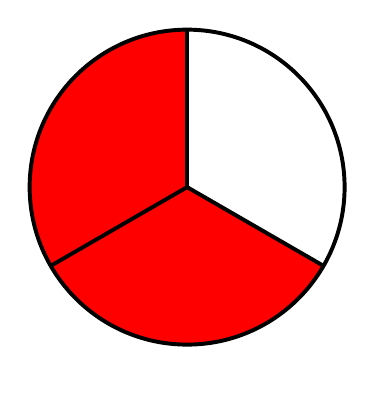
\begin{tikzpicture}
	\fill[red] (0,0) -- (0,2) arc (90:210:2cm) -- cycle;
	\fill[red] (0,0) -- (-2*0.8661,-2*0.5) arc (210:330:2cm) -- cycle;
	\draw[line width=0.5mm] (0,0) circle (2cm);
	\draw[line width=0.5mm] (0,0) -- (0,2);
	\draw[line width=0.5mm] (0,0) -- (2*0.8661,-2*0.5);
	\draw[line width=0.5mm] (0,0) -- (-2*0.8661,-2*0.5);
\end{tikzpicture}
\captionof{figure}{Red pieces in the pie represent $\frac{2}{3}$}
\end{center}

There are more ways to represent fractions graphically. For example:

\begin{center}
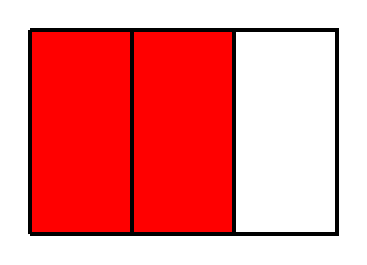
\begin{tikzpicture}
\draw[fill=red,line width=0.5mm] (0,0) -- (1.3*2,0) -- (1.3*2,1.3*2) -- (0,1.3*2);
\draw[line width=0.5mm] (1.3*1,0) -- (1.3*1,1.3*2);
\draw[line width=0.5mm] (0,0) -- (0,1.3*2);
\draw[line width=0.5mm] (1.3*2,0) -- (1.3*3,0) -- (1.3*3,1.3*2) -- (1.3*2,1.3*2);
\end{tikzpicture}
\captionof{figure}{Red pieces in the rectangle represent $\frac{2}{3}$}
\end{center}

Depending on the situations, we will use different shapes to represent fractions.

\subsection{Equivalent Fractions}
Let's look at the following two graphs:

\begin{center}
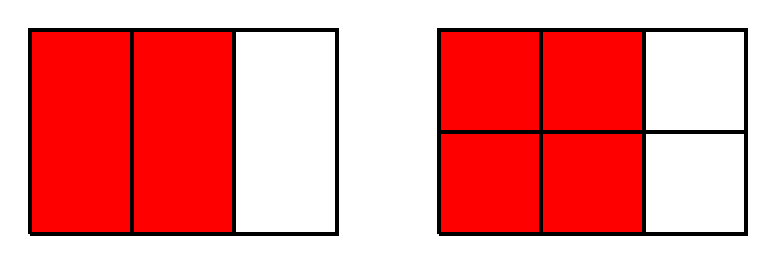
\begin{tikzpicture}

\draw[fill=red,line width=0.5mm] (0,0) -- (1.3*2,0) -- (1.3*2,1.3*2) -- (0,1.3*2) -- (0,0);
\draw[line width=0.5mm] (1.3*1,0) -- (1.3*1,1.3*2);
\draw[line width=0.5mm] (1.3*2,0) -- (1.3*3,0) -- (1.3*3,1.3*2) -- (1.3*2,1.3*2);

\draw[fill=red,line width=0.5mm] (1.3*4,0) -- (1.3*6,0) -- (1.3*6,1.3*2) -- (1.3*4,1.3*2) -- (1.3*4,0);
\draw[line width=0.5mm] (1.3*5,0) -- (1.3*5,1.3*2);
\draw[line width=0.5mm] (1.3*4,1.3*1) -- (1.3*7,1.3*1);
\draw[line width=0.5mm] (1.3*6,0) -- (1.3*7,0) -- (1.3*7,1.3*2) -- (1.3*6,1.3*2);

\end{tikzpicture}
\captionof{figure}{Compare $\frac{2}{3}$ and $\frac{4}{6}$}
\end{center}

The graph on the left side represents $\frac{2}{3}$, and the graph on the right side represents $\frac{4}{6}$. We can see they actually cover the same area. In other words:
\[ \frac{2}{3}=\frac{4}{6} \]

The difference is that the rectangle on the right side is cut into twice as many pieces as the rectangle on the left side. Let's look at this equation:
\[ \frac{2}{3}=\frac{2\cdot2}{3\cdot2}=\frac{4}{6} \]

To change $\frac{2}{3}$ to $\frac{4}{6}$, we multiply $2$ in both the numerator and denominator. This implies we cut the rectangle into twice as many pieces ($6$), and take twice as many pieces ($4$). The value of the fraction didn't change!

For $\frac{2}{3}$, if we cut the rectangle into $3$ times as many pieces, and take $3$ times as many pieces, the fraction's value would not change, either:
\[ \frac{2}{3}=\frac{2\cdot3}{3\cdot3}=\frac{6}{9} \]

Let's look at a graphic representation of this equation:

\begin{center}
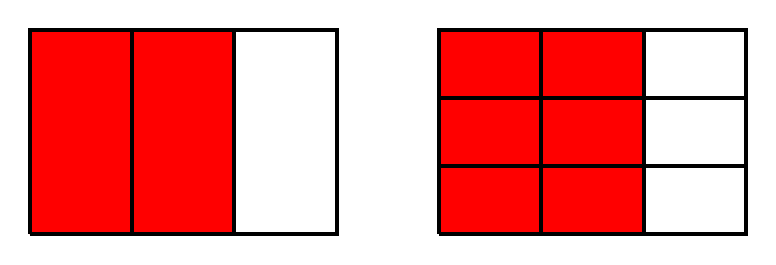
\begin{tikzpicture}

\draw[fill=red,line width=0.5mm] (0,0) -- (1.3*2,0) -- (1.3*2,1.3*2) -- (0,1.3*2) -- (0,0);
\draw[line width=0.5mm] (1.3*1,0) -- (1.3*1,1.3*2);
\draw[line width=0.5mm] (1.3*2,0) -- (1.3*3,0) -- (1.3*3,1.3*2) -- (1.3*2,1.3*2);

\draw[fill=red,line width=0.5mm] (1.3*4,0) -- (1.3*6,0) -- (1.3*6,1.3*2) -- (1.3*4,1.3*2) -- (1.3*4,0);
\draw[line width=0.5mm] (1.3*5,0) -- (1.3*5,1.3*2);
\draw[line width=0.5mm] (1.3*4,1.3*2/3) -- (1.3*7,1.3*2/3);
\draw[line width=0.5mm] (1.3*4,1.3*4/3) -- (1.3*7,1.3*4/3);
\draw[line width=0.5mm] (1.3*6,0) -- (1.3*7,0) -- (1.3*7,1.3*2) -- (1.3*6,1.3*2);

\end{tikzpicture}
\captionof{figure}{$\frac{2}{3}$ = $\frac{6}{9}$}
\end{center}

Here is the rule: If we multiply the same number in both the numerator and denominator of a fraction, the fraction's value doesn't change. For example, $\frac{2}{3}=\frac{2\cdot2}{3\cdot2}=\frac{4}{6}$, and $\frac{2}{3}=\frac{2\cdot3}{3\cdot3}=\frac{6}{9}$.

\begin{myexample}
Write a few equivalent fractions of $\frac{4}{5}$.
\end{myexample}
\begin{solution}
\[
\begin{aligned}[t]
   &\frac{4}{5}=\frac{4\cdot2}{5\cdot2}=\frac{8}{10} \\
   &\frac{4}{5}=\frac{4\cdot3}{5\cdot3}=\frac{12}{15} \\
   &\frac{4}{5}=\frac{4\cdot4}{5\cdot4}=\frac{16}{20} \\
   &\frac{4}{5}=\frac{4\cdot5}{5\cdot5}=\frac{20}{25} \\
   &...
\end{aligned}
\]
\end{solution}

\begin{myexample}
Change $\frac{2}{3}$ to an equivalent fraction with the denominator of $12$.
\end{myexample}
\begin{solution}
The question asks:
\[ \frac{2}{3}=\frac{?}{12} \]
To change the denominator from $3$ to $12$, we need to do $3\cdot4=12$. If we multiply the denominator with $4$, we must do the same to the numerator. We have:
\[ \frac{2}{3}=\frac{2\cdot4}{3\cdot4}=\frac{8}{12} \]
\end{solution}

Similarly, we can reduce fractions by dividing the same number in both the numerator and denominator:
\[
\begin{aligned}[t]
   &\frac{4}{6}=\frac{4\div2}{6\div2}=\frac{2}{3} \\
   &\frac{6}{9}=\frac{6\div3}{9\div3}=\frac{2}{3} \\
   &\frac{20}{25}=\frac{20\div5}{25\div5}=\frac{4}{5} \\
   &...
\end{aligned}
\]

How do we know which number to divide when we reduce fractions? Think about prime numbers: $2,3,5,7,11...$. Try prime numbers one by one.

\begin{myexample}
Reduce the fraction $\frac{30}{36}$.
\end{myexample}
\begin{solution}
\[
\begin{aligned}[t]
   &\phantom{{}=} \frac{24}{36} \\
   &= \frac{24\div2}{36\div2} &\phantom{=====}\text{2 goes into both 24 and 36.} \\
   &= \frac{12}{18} \\
   &= \frac{12\div2}{18\div2} &\phantom{=====}\text{2 goes into both 12 and 18.} \\
   &= \frac{6}{9} \\
   &= \frac{6\div3}{9\div3} &\phantom{=====}\text{3 goes into both 6 and 9.} \\
   &= \frac{2}{3} &\text{No more prime numbers go into both 2 and 3.}\\
\end{aligned}
\]
\end{solution}

You only need to memorize the first $5$ prime numbers: $2,3,5,7,11$. Rarely would an instructor expect you to see the prime number $13$ goes into two numbers. Actually, to see whether $7$ goes into a number, usually we resort to a calculator.

If we can reduce a fraction, we must do so! We don't allow reducible fractions like $\frac{2}{4}$ and $\frac{3}{9}$ as the final answer of a problem. 

There is an easier way to reduce $\frac{24}{36}$:
\[ \frac{24}{36}=\frac{24\div12}{36\div12}=\frac{2}{3} \]
If you can see $12$ goes into both $24$ and $36$, you can reduce $\frac{24}{36}$ in one step. However, if you cannot see it, simply go through the list of prime numbers one by one, $2,3,5,7,11...$, you can still reduce $\frac{24}{36}$ to $\frac{2}{3}$.

\begin{myexample}
Reduce the fraction $\frac{42}{126}$.
\end{myexample}
\begin{solution}
\[
\begin{aligned}[t]
   &\phantom{{}=} \frac{42}{126} \\
   &= \frac{42\div2}{126\div2} &\phantom{=====}\text{2 goes into both 42 and 126.} \\
   &= \frac{21}{63} \\
   &= \frac{21\div3}{63\div3} &\phantom{=====}\text{3 goes into both 21 and 63.} \\
   &= \frac{7}{21} \\
   &= \frac{7\div7}{21\div7} &\phantom{=====}\text{7 goes into both 7 and 21.} \\
   &= \frac{1}{3}\\
\end{aligned}
\]
\end{solution}

Here are a few special cases in fraction reduction. Remember: The fraction line has the same function as the division symbol.

\[
\begin{aligned}[t]
   &\frac{10}{10}=10\div10=1 \\
   &\frac{10}{1}=10\div1=10 \\
   &\frac{10}{0}=10\div0=\text{undefined} \\
   &\frac{0}{10}=0\div10=0 \\
\end{aligned}
\]

We can easily change a fraction to a decimal with a simple division: $\frac{1}{2}=1\div2=0.5$. We will cover this in the decimal chapter.

\subsection{Compare Fractions}
It's easy to understand that $\frac{2}{3}>\frac{1}{3}$, and $\frac{3}{10}<\frac{7}{10}$. How would we compare fractions when the denominators are different? Like $\frac{5}{6}$ and $\frac{7}{8}$?

Now that we learned how to change a fraction to its equivalent, we can change the denominators to the same number and then compare them.

\begin{myexample}
Compare $\frac{5}{6}$ and $\frac{7}{8}$.
\label{ex:u3l1CompareFractions}
\end{myexample}
\begin{solution}
Since $6\cdot8=48$, we know both $6$ and $8$ go into $48$, so we will change both denominators to $48$:
\[ \frac{5}{6} = \frac{5\cdot8}{6\cdot8} = \frac{30}{48} \text{ and } \frac{7}{8} = \frac{7\cdot6}{8\cdot6} = \frac{42}{48} \]

\textbf{Conclusion:} Now we can tell $\frac{5}{6}<\frac{7}{8}$.

If you can see both $6$ and $8$ go into $24$, you can avoid dealing with bigger numbers, but the result would be the same. In that case, you would do:
\[ \frac{5}{6} = \frac{5\cdot4}{6\cdot4} = \frac{20}{24} \text{ and } \frac{7}{8} = \frac{7\cdot3}{8\cdot3} = \frac{21}{24} \]

The conclusion stays the same: $\frac{7}{8}$ is bigger.
\end{solution}

\subsection{Fractions on Number Line}
The following figures show how to locate fractions on the number line. These figures are pretty self-explanatory. We need to count each unit (from 0 to 1) is cut into how many segments.

\begin{center}
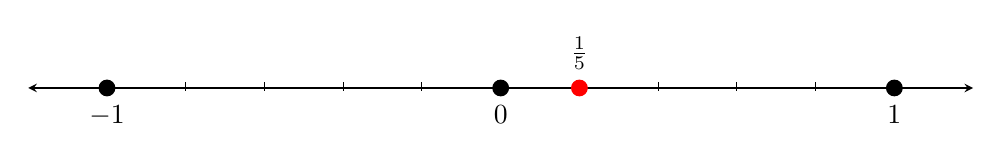
\begin{tikzpicture}
% a straight line segment
\draw [<->] (0,0) -- (12,0);
% the ticks and their labels
\foreach \x  in {1,...,11}
  \draw[xshift=\x cm] (0pt,2pt) -- (0pt,-1pt);
\node[fill=black,draw=black,circle,inner sep=2pt,label=below:{$0$}] at (6,0) {};
\node[fill=black,draw=black,circle,inner sep=2pt,label=below:{$1$}] at (11,0) {};
\node[fill=black,draw=black,circle,inner sep=2pt,label=below:{$-1$}] at (1,0) {};
\node[fill=red,draw=red,circle,inner sep=2pt,label=above:{$\frac{1}{5}$}] at (7,0) {};
\end{tikzpicture}

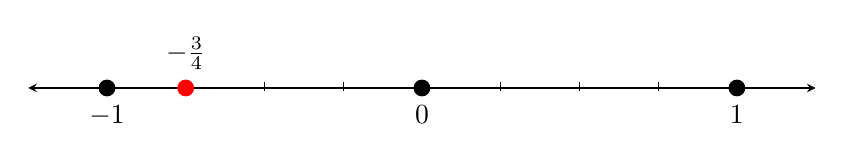
\begin{tikzpicture}
% a straight line segment
\draw [<->] (0,0) -- (10,0);
% the ticks and their labels
\foreach \x  in {1,...,9}
  \draw[xshift=\x cm] (0pt,2pt) -- (0pt,-1pt);
\node[fill=black,draw=black,circle,inner sep=2pt,label=below:{$0$}] at (5,0) {};
\node[fill=black,draw=black,circle,inner sep=2pt,label=below:{$1$}] at (9,0) {};
\node[fill=black,draw=black,circle,inner sep=2pt,label=below:{$-1$}] at (1,0) {};
\node[fill=red,draw=red,circle,inner sep=2pt,label=above:{$-\frac{3}{4}$}] at (2,0) {};
\end{tikzpicture}

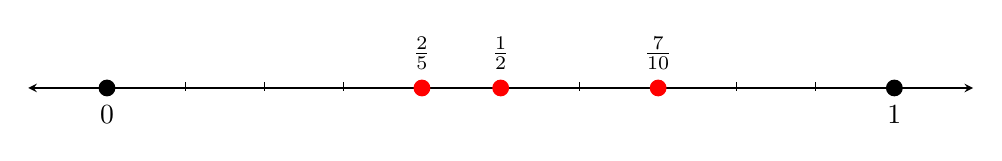
\begin{tikzpicture}
% a straight line segment
\draw [<->] (0,0) -- (12,0);
% the ticks and their labels
\foreach \x  in {1,...,11}
  \draw[xshift=\x cm] (0pt,2pt) -- (0pt,-1pt);
\node[fill=black,draw=black,circle,inner sep=2pt,label=below:{$0$}] at (1,0) {};
\node[fill=black,draw=black,circle,inner sep=2pt,label=below:{$1$}] at (11,0) {};
\node[fill=red,draw=red,circle,inner sep=2pt,label=above:{$\frac{7}{10}$}] at (8,0) {};
\node[fill=red,draw=red,circle,inner sep=2pt,label=above:{$\frac{1}{2}$}] at (6,0) {};
\node[fill=red,draw=red,circle,inner sep=2pt,label=above:{$\frac{2}{5}$}] at (5,0) {};
\end{tikzpicture}
\captionof{figure}{Locate fractions on number line}

\end{center}

On the last number line, note that the segment from $0$ to $1$ is cut evenly into $10$ pieces, implying each piece represents $\frac{1}{10}$. The first red dot is $4$ pieces away from $0$, which represents $\frac{4}{10}$. We must reduce the fraction: $\frac{4}{10}=\frac{2}{5}$.

Similarly, the second red dot represents $\frac{5}{10}$. We must again reduce the fraction: $\frac{5}{10}=\frac{1}{2}$.

The third red dot represents $\frac{7}{10}$. We cannot reduce this fraction.

\subsection{Summary}
Let's review what we learned in this lesson:
\begin{itemize}
\item To understand a fraction like $\frac{2}{3}$, we look at the denominator $3$ first, and then look at the numerator $2$. For $\frac{2}{3}$, we cut the whole evenly into $3$ pieces, and then take $2$ of those pieces.
\item If we multiply the same number in both the numerator and denominator of a fraction, the fraction's value doesn't change. For example, 
\[ \frac{2}{3}=\frac{2\cdot2}{3\cdot2}=\frac{4}{6} \]
\item If we divide the same number in both the numerator and denominator of a fraction, the fraction's value doesn't change. For example, 
\[ \frac{4}{6}=\frac{4\div2}{6\div2}=\frac{2}{3} \]
\item When we compare two fractions with different denominators, we can change the denominators to the same number, and then compare the numerators, like in \cref{ex:u3l1CompareFractions}.
\end{itemize}

\section{Add/Subtract Fractions}

In this lesson, we will learn how to add and subtract fractions.

\subsection{Add/Subtract Fractions with the Same Denominator}

We will do $\frac{1}{3}+\frac{1}{3}$ by graphing:

\begin{center}
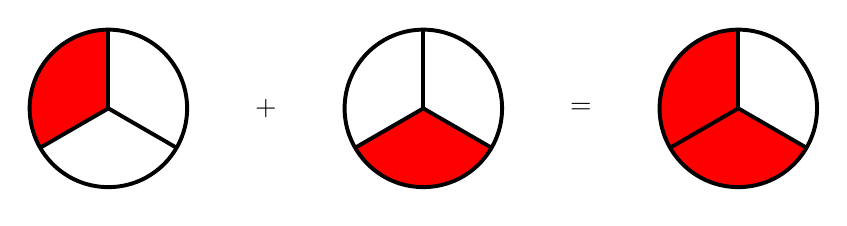
\begin{tikzpicture}
	\fill[red] (0,0) -- (0,1) arc (90:210:1cm) -- cycle;
	\draw[line width=0.5mm] (0,0) circle (1cm);
	\draw[line width=0.5mm] (0,0) -- (0,1);
	\draw[line width=0.5mm] (0,0) -- (0.8661,-0.5);
	\draw[line width=0.5mm] (0,0) -- (-0.8661,-0.5);
	
	\draw (2,0) node{+};
	
	\fill[red] (4,0) -- (-0.8661+4,-0.5) arc (210:330:1cm) -- cycle;
	\draw[line width=0.5mm] (4,0) circle (1cm);
	\draw[line width=0.5mm] (4,0) -- (4,1);
	\draw[line width=0.5mm] (4,0) -- (0.8661+4,-0.5);
	\draw[line width=0.5mm] (4,0) -- (-0.8661+4,-0.5);
	
	\draw (6,0) node{=};
	
	\fill[red] (8,0) -- (8,1) arc (90:210:1cm) -- cycle;
	\fill[red] (8,0) -- (-0.8661+8,-0.5) arc (210:330:1cm) -- cycle;
	\draw[line width=0.5mm] (8,0) circle (1cm);
	\draw[line width=0.5mm] (8,0) -- (8,1);
	\draw[line width=0.5mm] (8,0) -- (0.8661+8,-0.5);
	\draw[line width=0.5mm] (8,0) -- (-0.8661+8,-0.5);
	
\end{tikzpicture}
\captionof{figure}{$\frac{1}{3}+\frac{1}{3}=\frac{2}{3}$}
\end{center}

It's easy to see $\frac{1}{3}+\frac{1}{3}=\frac{2}{3}$. When we add fractions, we simply add the numerators, but the denominator doesn't change. The same rule applies when we subtract fractions.

\begin{myexample}
\[ 
\begin{aligned}[t]
	&\phantom{{}=}\frac{1}{5}+\frac{2}{5}+\frac{2}{5} \\
	&= \frac{1+2+2}{5} \\
	&= \frac{5}{5} \\
	&= 1
\end{aligned}
\]
\end{myexample}

\begin{myexample}
\[ 
\begin{aligned}[t]
	&\phantom{{}=}\frac{4}{5}-\frac{2}{5}+\frac{1}{5} \\
	&= \frac{4-2+1}{5} \\
	&= \frac{3}{5}
\end{aligned}
\]
\end{myexample}

\subsection{Add/Subtract Fractions with Different Denominator}
We will use $\frac{1}{2}+\frac{1}{4}$ as an example. First, we will do this in the "easy" way (wrong way):
\[ 
\begin{aligned}[t]
	&\phantom{{}=}\frac{1}{2}+\frac{1}{4} \\
	&=\frac{1+1}{2+4} \\
	&=\frac{2}{6} \\
	&=\frac{1}{3} 
\end{aligned}
\]

If we simply add the numerators and denominators, like what we did, it doesn't make sense. If we add up $\frac{1}{2}$ and $\frac{1}{4}$, the answer cannot be $\frac{1}{3}$, because $\frac{1}{3}$ is smaller than $\frac{1}{2}$. We must change the denominators to the same number, before adding up the numerators.

Earlier, we learned how to find the LCM (Least Common Multiple) of a group of numbers. This is a good opportunity to go back and review that lesson.

Since $2$ goes into $4$, the LCM of $2$ and $4$ is simply $4$. To change $\frac{1}{2}$ to $\frac{?}{4}$, we multiply $2$ in both the numerator and denominator of $\frac{1}{2}$. The full solution is:
\[ 
\begin{aligned}[t]
	&\phantom{{}=}\frac{1}{2}+\frac{1}{4} \\
	&=\frac{1\cdot2}{2\cdot2}+\frac{1}{4} \\
	&=\frac{2}{4}+\frac{1}{4} \\
	&=\frac{2+1}{4} \\
	&=\frac{3}{4} 
\end{aligned}
\]
This result makes sense because half a dollar (50 cents) plus a quarter (25 cents) is three quarters (75 cents). Let's understand this problem by graph:

\begin{center}
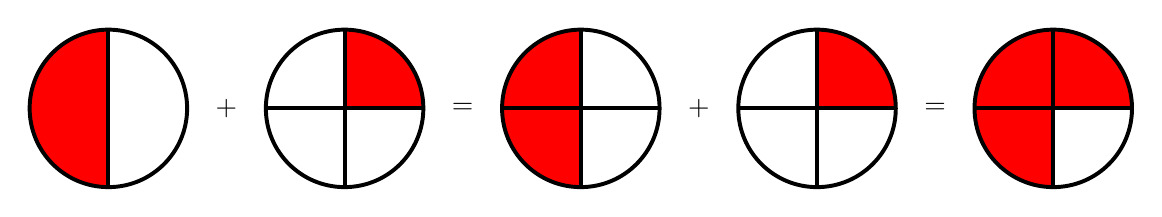
\begin{tikzpicture}
	\fill[red] (0,0) -- (0,1) arc (90:270:1cm) -- cycle;
	\draw[line width=0.5mm] (0,0) circle (1cm);
	\draw[line width=0.5mm] (0,-1) -- (0,1);
	
	\draw (1.5,0) node{+};
	
	\fill[red] (0+3,0) -- (0+3,1) arc (90:0:1cm) -- cycle;
	\draw[line width=0.5mm] (0+3,0) circle (1cm);
	\draw[line width=0.5mm] (-1+3,0) -- (1+3,0);
	\draw[line width=0.5mm] (0+3,-1) -- (0+3,1);
	
	\draw (4.5,0) node{=};
	
	\fill[red] (0+6,0) -- (0+6,1) arc (90:270:1cm) -- cycle;
	\draw[line width=0.5mm] (0+6,0) circle (1cm);
	\draw[line width=0.5mm] (-1+6,0) -- (1+6,0);
	\draw[line width=0.5mm] (0+6,-1) -- (0+6,1);
	
	\draw (7.5,0) node{+};
	
	\fill[red] (0+9,0) -- (0+9,1) arc (90:0:1cm) -- cycle;
	\draw[line width=0.5mm] (0+9,0) circle (1cm);
	\draw[line width=0.5mm] (-1+9,0) -- (1+9,0);
	\draw[line width=0.5mm] (0+9,-1) -- (0+9,1);
	
	\draw (10.5,0) node{=};
	
	\fill[red] (0+12,0) -- (0+12,1) arc (90:270:1cm) -- cycle;
	\fill[red] (0+12,0) -- (0+12,1) arc (90:0:1cm) -- cycle;
	\draw[line width=0.5mm] (0+12,0) circle (1cm);
	\draw[line width=0.5mm] (-1+12,0) -- (1+12,0);
	\draw[line width=0.5mm] (0+12,-1) -- (0+12,1);
	
\end{tikzpicture}
\captionof{figure}{$\frac{1}{2}+\frac{1}{4}=\frac{3}{4}$}
\end{center}

In the graph, the first step is to cut $\frac{1}{2}$ into twice as many pieces, which changes $\frac{1}{2}$ into $\frac{2}{4}$. Understand that when we do $\frac{1}{2}=\frac{1\cdot2}{2\cdot2}=\frac{2}{4}$, we are simply cutting the whole into more pieces without changing the fraction's value.

The rule is the same when we subtract fractions with different denominators.

\begin{myexample}
\[ 
\begin{aligned}[t]
	&\phantom{{}=}\frac{1}{2}-\frac{1}{3} \\
	&=\frac{1\cdot3}{2\cdot3}-\frac{1\cdot2}{3\cdot2} \\
	&=\frac{3}{6}-\frac{2}{6} \\
	&=\frac{3-2}{6} \\
	&=\frac{1}{6} 
\end{aligned}
\]
The LCM of $2$ and $3$ is $6$.
\end{myexample}

If the answer can be reduced, we must do so, as in the next example.

\begin{myexample}
\[ 
\begin{aligned}[t]
	&\phantom{{}=}\frac{1}{2}-\frac{1}{6} \\
	&=\frac{1\cdot3}{2\cdot3}-\frac{1}{6} \\
	&=\frac{3}{6}-\frac{1}{6} \\
	&=\frac{3-1}{6} \\
	&=\frac{2}{6} \\
	&=\frac{2\div2}{6\div2} \\
	&=\frac{1}{3} 
\end{aligned}
\]
In the last step, we must reduce $\frac{2}{6}$ to $\frac{1}{3}$. Make it a habit to check whether a fraction can be reduced. Try the first few prime numbers: $2,3,5,7,11$.
\end{myexample}

\subsection{Fraction Word Problems}
\begin{myexample}
Omar and Jose are painting a room. Omar can paint the whole room in $8$ hours if he works by himself, while Jose can paint the whole room in $4$ hours. If they work together, what fraction of the job can be done in one hour?
\end{myexample}
\begin{solution}
Since Omar can paint the whole room in $8$ hours, he can complete $\frac{1}{8}$ of the job in one hour.

Similarly, Jose can complete $\frac{1}{4}$ of the job in one hour.

To find what fraction of the job can be done if they work together, we add up the fraction of the job each person can complete:
\[ 
\begin{aligned}[t]
	&\phantom{{}=}\frac{1}{8}+\frac{1}{4} \\
	&=\frac{1}{8}+\frac{1\cdot2}{4\cdot2} \\
	&=\frac{1}{8}+\frac{2}{8} \\
	&=\frac{1+2}{8} \\
	&=\frac{3}{8} 
\end{aligned}
\]
If they work together, $\frac{3}{8}$ of the job can be done in one hour.
\end{solution}

\begin{myexample}
Tom, Jerry and Peter are sharing a pizza. Tom ate $\frac{2}{5}$ of the pizza; Jerry ate $\frac{1}{4}$ of the pizza; Peter ate the rest. What fraction of the pizza did Peter eat?
\end{myexample}
\begin{solution}
The whole pizza is a whole $1$. After Tom ate $\frac{2}{5}$ and Jerry ate $\frac{1}{4}$, what's left is:
\[ 
\begin{aligned}[t]
	&\phantom{{}=}1-\frac{2}{5}-\frac{1}{4} \\
	&=\frac{1}{1}-\frac{2}{5}-\frac{1}{4} \\
	&=\frac{1\cdot20}{1\cdot20}-\frac{2\cdot4}{5\cdot4}-\frac{1\cdot5}{4\cdot5} \\
	&=\frac{20}{20}-\frac{8}{20}-\frac{5}{20} \\
	&=\frac{7}{20} \\
\end{aligned}
\]
Peter ate $\frac{7}{20}$ of the pizza.

Note that the LCM of $1$, $5$ and $4$ is $20$.
\end{solution}

\subsection{Summary}
Let's review what we learned in this lesson:
\begin{itemize}
\item To add/subtract fractions with the same denominator, we add/subtract the numerators, and keep the denominator unchanged. For example: 
\[ \frac{3}{5}+\frac{1}{5}=\frac{3+1}{5}=\frac{4}{5} \]
\item To add/subtract fractions with different denominators, first change the denominator to the same number (their LCM), and then add/subtract the numerators. For example: 
\[ \frac{1}{2}+\frac{1}{3}=\frac{1\cdot3}{2\cdot3}+\frac{1\cdot2}{3\cdot2}=\frac{3}{6}+\frac{2}{6}=\frac{3+2}{6}=\frac{5}{6} \]
\end{itemize}



\section{Multiply Fractions}

In this lesson, we will learn how to multiply fractions.

\subsection{Multiply Two Fractions}

We will start with a very important concept: The English word "of," in many cases, can be translated into the multiplication sign in math. For example, "twice of $5$" can be translated into $2\cdot5$.

Similarly, "half of half a dollar (50 cents)" can be translated into $\frac{1}{2}\cdot\frac{1}{2}$. We know the answer should be 25 cents, or $\frac{1}{4}$. We have:
\[ \frac{1}{2}\cdot\frac{1}{2}=\frac{1}{4} \]

We can see how to multiply fractions: We simply multiply the numerators and denominators. This is much easier than adding fractions---There is no need to find the common denominator when we multiply fractions.

\begin{myexample}
\[ 
\begin{aligned}[t]
	&\phantom{{}=}\frac{2}{3} \cdot \frac{2}{5} \\
	&= \frac{2\cdot2}{3\cdot5} \\
	&= \frac{4}{15}
\end{aligned}
\]
\end{myexample}

Remember: We must reduce fraction if we can. See the next example.

\begin{myexample}
\[ 
\begin{aligned}[t]
	&\phantom{{}=}\frac{2}{3} \cdot \frac{3}{5} \\
	&= \frac{2\cdot3}{3\cdot5} \\
	&= \frac{6}{15} \\
	&= \frac{6\div3}{15\div3} \\
	&= \frac{2}{5}
\end{aligned}
\]
In the example above, we could reduce fractions before we multiply across:
\[ 
\begin{aligned}[t]
	&\phantom{{}=}\frac{2}{3} \cdot \frac{3}{5} \\
	&= \frac{2}{3\div3} \cdot \frac{3\div3}{5} \\
	&= \frac{2}{1} \cdot \frac{1}{5} \\
	&= \frac{2\cdot1}{1\cdot5} \\
	&= \frac{2}{5}
\end{aligned}
\]
This skill will save us a lot of time if numbers are big. See the next example.
\end{myexample}

\begin{myexample}
\[ 
\begin{aligned}[t]
	&\phantom{{}=}\frac{4}{5} \cdot \frac{3}{8} \cdot \frac{5}{9} \\
	&= \frac{4{\color{red}\div4}}{5\color{blue}\div5} \cdot \frac{3\color{brown}\div3}{8\color{red}\div4} \cdot \frac{5\color{blue}\div5}{9\color{brown}\div3} \\
	&= \frac{1}{1} \cdot \frac{1}{2} \cdot \frac{1}{3} \\
	&= \frac{1\cdot1\cdot1}{1\cdot2\cdot3} \\
	&= \frac{1}{6}
\end{aligned}
\]
In this example, if we don't reduce fractions first, we have to deal with big numbers like $4\cdot3\cdot5=60$ and $5\cdot8\cdot9=360$.
\end{myexample}

Here is a common mistake:
\[
\begin{aligned}[t]
	&\phantom{{}=}\frac{2}{3}\cdot\frac{2}{5} \\
	&=\frac{2\div2}{3}\cdot\frac{2\div2}{5} \\
	&=\frac{1}{3}\cdot\frac{1}{5} \\
	&=\frac{1}{15}
\end{aligned}
\]
This is incorrect. When we reduce a fraction, we must divide a number in both the numerator and denominator. We cannot divide a number in two numerators, as in the example above. The correct answer is $\frac{2}{3}\cdot\frac{2}{5}=\frac{4}{15}$.

\subsection{Multiply a Fraction and an Integer}
When we multiply a fraction and an integer, we need to change the integer to a fraction, and then multiply two fractions.

\begin{myexample}
\[ 
\begin{aligned}[t]
	&\phantom{{}=}\frac{2}{9} \cdot 2 \\
	&= \frac{2}{9} \cdot \frac{2}{1} \\
	&= \frac{2\cdot2}{9\cdot1} \\
	&= \frac{4}{9}
\end{aligned}
\]
We can change $2$ into $\frac{2}{1}$ because $2\div1=2$.
\label{ex:MultiplyFraction1}
\end{myexample}

We need to learn an important shortcut, which will save you tons of time later. Recall that the fraction line is the same as the division symbol. We can do:
\[ \frac{3}{5}\cdot{10} = 10\div5\cdot3 = 2\cdot3=6 \]
Let's look at a few more examples:
\[
\begin{aligned}[t]
	&\frac{2}{3}\cdot{3}=3\div3\cdot2=1\cdot2=2 \\
	&\frac{2}{3}\cdot{6}=6\div3\cdot2=2\cdot2=4 \\
	&\frac{2}{3}\cdot{9}=9\div3\cdot2=3\cdot2=6 \\
\end{aligned}
\]

This shortcut works as long as the denominator goes into the integer evenly. If not, we have to change the integer to a fraction, and then do fraction multiplication like in \cref{ex:MultiplyFraction1}.

\subsection{Fraction Multiplication Word Problems}
\begin{myexample}
A school won a \$$5,000$ grant, and will use $\frac{3}{4}$ of the grant to purchase graphing calculators. How much money will be used to purchase graphing calculators?
\end{myexample}
\begin{solution}
This problem can be boiled down to this question: What is $\frac{3}{4}$ of $5,000$? Again, the word "of" can be translated into the multiplication sign in math. We have:
\[ 
\begin{aligned}[t]
	&\phantom{{}=}\frac{3}{4} \cdot 5000 \\
	&= 5000\div4\cdot3 \\
	&= 1250\cdot3 \\
	&= 3750
\end{aligned}
\]
We can use the shortcut to do fraction multiplication because the denominator $4$ goes into $5000$ evenly.

\textbf{Conclusion:} The school will spend \$$3,750$ to purchase graphing calculators.
\end{solution}

\begin{myexample}
A school won a grant, and will evenly share the grant among $8$ classes. In one class, Mr. Smith will use $\frac{2}{3}$ of the money for the class to purchase books. Mr. Smith will use what fraction of the school's grant to purchase books?
\end{myexample}
\begin{solution}
Since the grant is evenly shared by $8$ classes, each class gets $\frac{1}{8}$ of the grant.

Now this problem can be boiled down to this question: What is $\frac{2}{3}$ of $\frac{1}{8}$? Again, the word "of" can be translated into the multiplication sign in math. We have:
\[ 
\begin{aligned}[t]
	&\phantom{{}=}\frac{2}{3} \cdot \frac{1}{8} \\
	&= \frac{2\div2}{3} \cdot \frac{1}{8\div2} \\
	&= \frac{1}{3} \cdot \frac{1}{4} \\
	&= \frac{1\cdot1}{3\cdot4} \\
	&= \frac{1}{12}
\end{aligned}
\]
\textbf{Conclusion:} Mr. Smith will use $\frac{1}{12}$ of the school's grant to purchase books.
\end{solution}

\subsection{Summary}
Let's review what we learned in this lesson:
\begin{itemize}
\item To multiply two fractions, we simply multiply the numerators and  denominators. For example: 
\[ \frac{1}{2} \cdot \frac{1}{3}=\frac{1\cdot1}{2\cdot3}=\frac{1}{6} \]
\item When we multiply fractions, if we can reduce fractions before multiplying the numerators and denominators, we should reduce fractions first. This will avoid dealing with big numbers. For example:
\[ \frac{4}{7} \cdot \frac{3}{8} = \frac{4\div4}{7} \cdot \frac{3}{8\div4} = \frac{1}{7} \cdot \frac{3}{2} = \frac{3}{14} \]
\item To multiply a fraction and an integer, we first change the integer to a fraction, and then multiply the numerators and denominators. For example:
\[ \frac{1}{3} \cdot 2 = \frac{1}{3} \cdot \frac{2}{1} = \frac{2}{3} \]
\item When we multiply a fraction and an integer, if the denominator can go into the integer evenly, there is a shortcut:
\[ \frac{2}{3} \cdot 6 = 6 \div 3 \cdot 2 = 2 \cdot 2 = 4 \]
\end{itemize}



\section{Divide Fractions}
\thispagestyle{fancy}

In this lesson, we will learn how to divide fractions.

\subsection{Understand Dividing Fractions}

How many quarters are there in \$$3.00$? This is a division problem:
\[ 3\div\frac{1}{4} \]
To do this problem, we divide all \$$3.00$ into quarters, and we will have $3\cdot4=12$ quarters. So the solution is $3\div\frac{1}{4}=12$.

Next, let's make this example more interesting:
\[ 3\div\frac{3}{4} \]
We need to find how many "three quarters" are in \$$3.00$? We will do this in two steps:
\begin{enumerate}
\item We divide $3$ into quarters, and we have $3\cdot4=12$ quarters.
\item We divide $12$ quarters into groups of $3$, and we have $12\div3=4$ groups.
\end{enumerate}
The solution is:
\[ 3\div\frac{3}{4}=3\cdot4\div3=12\div3=4 \]
Recall that the fraction line is the same as the division symbol. We can re-write the solution as:
\[ 3\div\frac{3}{4}=3\cdot\frac{4}{3}=\frac{3}{1}\cdot\frac{4}{3}=\frac{12}{3}=4 \]
The second way is how most middle school teachers teach dividing fractions: We change division to multiplication, and at the same time "flip" the second fraction. Unfortunately, the procedure doesn't make sense. I hope the money model helps you understand why the procedure makes sense.

I have to say it's rather difficult to understand fraction division. If you are not interested in understanding why, simply remember the rule.

\begin{myexample}
\[ 
\begin{aligned}[t]
	&\phantom{{}=}\frac{2}{3} \div \frac{2}{9} \\
	&= \frac{2}{3} \cdot \frac{9}{2} \\
	&= \frac{2\div2}{3\div3} \cdot \frac{9\div3}{2\div2} \\
	&= \frac{1}{1} \cdot \frac{3}{1} \\
	&= \frac{3}{1} \\
	&= 3
\end{aligned}
\]
Never let fractions like $\frac{3}{1}$ be the final answer! Change it to an integer.
\end{myexample}

\subsection{Dividing Fractions involving Integers}
If an integer is involved in fraction division, we first change the integer to a fraction by adding $1$ to the denominator. This is similar to the rule for fraction multiplication.

\begin{myexample}
\[ 
\begin{aligned}[t]
	&\phantom{{}=} 10 \div \frac{5}{9} \\
	&= \frac{10}{1} \div \frac{5}{9} \\
	&= \frac{10}{1} \cdot \frac{9}{5} \\
	&= \frac{10\div5}{1} \cdot \frac{9}{5\div5} \\
	&= \frac{2}{1} \cdot \frac{9}{1} \\
	&= \frac{18}{1} \\
	&= 18
\end{aligned}
\]
\end{myexample}

\begin{myexample}
\[ 
\begin{aligned}[t]
	&\phantom{{}=} \frac{5}{9} \div 10 \\
	&= \frac{5}{9} \div \frac{10}{1} \\
	&= \frac{5}{9} \cdot \frac{1}{10} \\
	&= \frac{5\div5}{9} \cdot \frac{1}{10\div5} \\
	&= \frac{1}{9} \cdot \frac{1}{2} \\
	&= \frac{1}{18}
\end{aligned}
\]
\end{myexample}

\subsection{Fraction Division Word Problems}
\begin{myexample}
A school won a grant, and will spend $\frac{2}{3}$ of it to purchase textbooks. Six committees will evenly share the textbook fund to purchase textbooks of $6$ subjects. What fraction of the total grant will be used by each committee to purchase textbooks?
\end{myexample}
\begin{solution}
In this problem, $\frac{2}{3}$ will be evenly divided into $6$ pieces, a division problem:
\[ 
\begin{aligned}[t]
	&\phantom{{}=} \frac{2}{3} \div 6 \\
	&= \frac{2}{3} \div \frac{6}{1} \\
	&= \frac{2}{3} \cdot \frac{1}{6} \\
	&= \frac{2\div2}{3} \cdot \frac{1}{6\div2} \\
	&= \frac{1}{3} \cdot \frac{1}{3} \\
	&= \frac{1}{9}
\end{aligned}
\]
\textbf{Conclusion:} Each committee will use $\frac{1}{9}$ of the total grant to purchase textbooks.
\end{solution}

\begin{myexample}
Jack will use his car to move a pile of rocks which weigh $\frac{7}{8}$ of a ton. Jack's car can load only $\frac{1}{16}$ of a ton. How many trips will it take to move the whole pile?
\end{myexample}
\begin{solution}
In this problem, we will repeatedly take away $\frac{1}{16}$ of a ton from $\frac{7}{8}$ of a ton, a division problem:
\[ 
\begin{aligned}[t]
	&\phantom{{}=} \frac{7}{8} \div \frac{1}{16} \\
	&= \frac{7}{8} \cdot \frac{16}{1} \\
	&= \frac{7}{8\div8} \cdot \frac{16\div8}{1} \\
	&= \frac{7}{1} \cdot \frac{2}{1} \\
	&= \frac{14}{1} \\
	&= 14
\end{aligned}
\]
\textbf{Conclusion:} It will take $14$ trips to move the whole pile of rocks.
\end{solution}


\subsection{Summary}
Let's review what we learned in this lesson:
\begin{itemize}
\item To divide two fractions, we change division to multiplication, and at the same time, flip the second fraction. For example: 
\[ \frac{1}{3} \div \frac{1}{2}= \frac{1}{3} \cdot \frac{2}{1} = \frac{2}{3} \]
\item If an integer is involved in fraction division, we first change the integer to a fraction, and then carry out the procedures above. For example:
\[ \frac{1}{3} \div 2 = \frac{1}{3} \div \frac{2}{1} = \frac{1}{3} \cdot \frac{1}{2} = \frac{1}{6} \]
\end{itemize}



\section{Introduction to Mixed Number}

In this lesson, we will learn the definition of mixed numbers, and how to convert between improper fraction (like $\frac{3}{2}$) and mixed number (like $1 \frac{1}{2}$).

\subsection{Definition of Mixed Number}

Let's review the definition of fractions, and use $\frac{2}{3}$ as an example. Remember, we should look at the denominator, $3$, first:
\begin{enumerate}
\item We cut the whole evenly into $3$ pieces.
\item We take $2$ of those pieces.
\end{enumerate}

\begin{center}
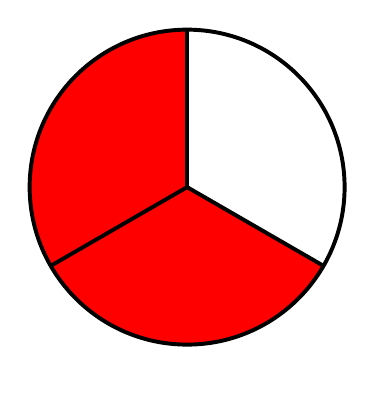
\begin{tikzpicture}
	\fill[red] (0,0) -- (0,2) arc (90:210:2cm) -- cycle;
	\fill[red] (0,0) -- (-2*0.8661,-2*0.5) arc (210:330:2cm) -- cycle;
	\draw[line width=0.5mm] (0,0) circle (2cm);
	\draw[line width=0.5mm] (0,0) -- (0,2);
	\draw[line width=0.5mm] (0,0) -- (2*0.8661,-2*0.5);
	\draw[line width=0.5mm] (0,0) -- (-2*0.8661,-2*0.5);
\end{tikzpicture}
\captionof{figure}{Red pieces in the pie represent $\frac{2}{3}$}
\end{center}

Let's use the same concept to draw $\frac{7}{3}$.
\begin{enumerate}
\item We cut the whole evenly into $3$ pieces.
\item We take $7$ of those pieces. Since one pie only has $3$ pieces, we need to cut more than one pie to have $7$ pieces.
\end{enumerate}

\begin{center}
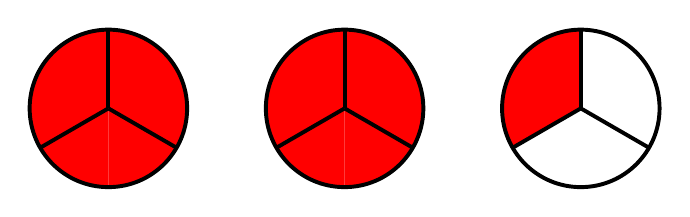
\begin{tikzpicture}
	\fill[red] (0,0) -- (0,1) arc (90:270:1cm) -- cycle;
	\fill[red] (0,0) -- (0,1) arc (90:-90:1cm) -- cycle;
	\draw[line width=0.5mm] (0,0) circle (1cm);
	\draw[line width=0.5mm] (0,0) -- (0,1);
	\draw[line width=0.5mm] (0,0) -- (0.8661,-0.5);
	\draw[line width=0.5mm] (0,0) -- (-0.8661,-0.5);
	
	\fill[red] (3,0) -- (3,1) arc (90:270:1cm) -- cycle;
	\fill[red] (3,0) -- (3,1) arc (90:-90:1cm) -- cycle;
	\draw[line width=0.5mm] (3,0) circle (1cm);
	\draw[line width=0.5mm] (3,0) -- (3,1);
	\draw[line width=0.5mm] (3,0) -- (0.8661+3,-0.5);
	\draw[line width=0.5mm] (3,0) -- (-0.8661+3,-0.5);
	
	\fill[red] (6,0) -- (6,1) arc (90:210:1cm) -- cycle;
	\draw[line width=0.5mm] (6,0) circle (1cm);
	\draw[line width=0.5mm] (6,0) -- (6,1);
	\draw[line width=0.5mm] (6,0) -- (0.8661+6,-0.5);
	\draw[line width=0.5mm] (6,0) -- (-0.8661+6,-0.5);
	
\end{tikzpicture}
\captionof{figure}{Red pieces represent $\frac{7}{3}$}
\end{center}

If the numerator is bigger than the denominator, like in $\frac{7}{3}$, this fraction is called an \textit{improper fraction}.

Another way to write $\frac{7}{3}$ is $2 \frac{1}{3}$, representing $2$ whole pies plus $\frac{1}{3}$ of a pie. A fraction like $2 \frac{1}{3}$ is called a \textit{mixed number}.

In other words, each mixed number can be converted to an improper fraction, and vice versa:
\[ \frac{7}{3} = 2\frac{1}{3} \]

\subsection{Convert between Improper Fractions and Mixed Numbers}
Let's look at one more example by graphing. Write a mixed number and an improper fraction for the following graph:

\begin{center}
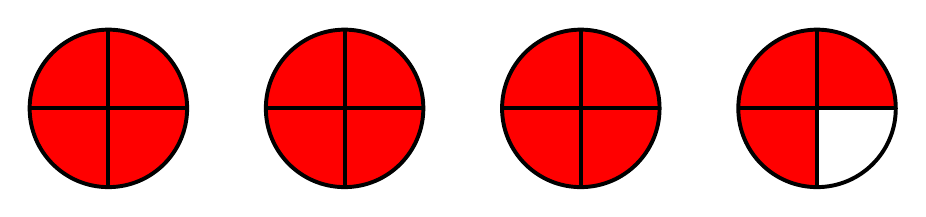
\begin{tikzpicture}
	\fill[red] (0,0) -- (0,1) arc (90:270:1cm) -- cycle;
	\fill[red] (0,0) -- (0,1) arc (90:-90:1cm) -- cycle;
	\draw[line width=0.5mm] (0,0) circle (1cm);
	\draw[line width=0.5mm] (-1,0) -- (1,0);
	\draw[line width=0.5mm] (0,1) -- (0,-1);
	
	\fill[red] (3,0) -- (3,1) arc (90:270:1cm) -- cycle;
	\fill[red] (3,0) -- (3,1) arc (90:-90:1cm) -- cycle;
	\draw[line width=0.5mm] (3,0) circle (1cm);
	\draw[line width=0.5mm] (-1+3,0) -- (1+3,0);
	\draw[line width=0.5mm] (0+3,1) -- (0+3,-1);
	
	\fill[red] (6,0) -- (6,1) arc (90:270:1cm) -- cycle;
	\fill[red] (6,0) -- (6,1) arc (90:-90:1cm) -- cycle;
	\draw[line width=0.5mm] (6,0) circle (1cm);
	\draw[line width=0.5mm] (-1+6,0) -- (1+6,0);
	\draw[line width=0.5mm] (0+6,1) -- (0+6,-1);
	
	\fill[red] (9,0) -- (9,1) arc (90:270:1cm) -- cycle;
	\fill[red] (9,0) -- (9,1) arc (90:0:1cm) -- cycle;
	\draw[line width=0.5mm] (9,0) circle (1cm);
	\draw[line width=0.5mm] (-1+9,0) -- (1+9,0);
	\draw[line width=0.5mm] (0+9,1) -- (0+9,-1);
	
\end{tikzpicture}
\captionof{figure}{A graph representing a mixed number}
\end{center}

In improper fraction format, the graph represents $\frac{15}{4}$, because there are $15$ pieces of a quarter.

In mixed number format, the graph represents $3\frac{3}{4}$.

This implies:
\[ \frac{15}{4} = 3\frac{3}{4}  \]

Let's look at both graphs and both conversions:
\[
\begin{aligned}[t]
	\frac{7}{3} &= 2\frac{1}{3} \\
	\frac{15}{4} &= 3\frac{3}{4}
\end{aligned}
\]

The fraction $\frac{7}{3}$ has two whole pies because $3$ goes into $7$ twice. The fraction part of $2\frac{1}{3}$ is $\frac{1}{3}$ because there is one extra piece, or $7\div3=2R1$ (remainder is $1$).

The fraction $\frac{15}{4}$ has three whole pies because $4$ goes into $15$ three times. The fraction part of $3\frac{3}{4}$ is $\frac{3}{4}$ because there are three extra pieces, or $15\div4=3R3$ (remainder is $3$).

Once the above explanation makes sense, we can convert between improper fractions and mixed numbers without graphing.

\begin{myexample}
Convert $\frac{19}{7}$ to a mixed number.
\end{myexample}
\begin{solution}
Since $19\div7=2R5$, it implies we can draw two whole pies, with each pie having $7$ pieces. There are still $5$ extra pieces, so we have:
\[ \frac{19}{7} = 2\frac{5}{7} \]
\end{solution}

\begin{myexample}
Convert $4\frac{3}{5}$ to a mixed number.
\end{myexample}
\begin{solution}
The mixed number's fraction part is $\frac{3}{5}$, implying each pie is cut into $5$ pieces.

Since there are $4$ whole pies, once each pie is cut into $5$ pieces, there are a total of $4\cdot5=20$ pieces.

The fraction part is $\frac{3}{5}$, implying there are $3$ extra pieces. Altogether, there are $4\cdot5+3=23$ pieces of one fifth of a pie. So we have: 
\[ 4\frac{3}{5} = \frac{4\cdot5+3}{5} = \frac{23}{5} \]
\end{solution}

\subsection{Mixed Numbers on Number Line}
The following figures show how to locate mixed numbers on the number line. These figures are pretty self-explanatory. We need to count each unit (like from 0 to 1) is cut into how many segments.

\begin{center}
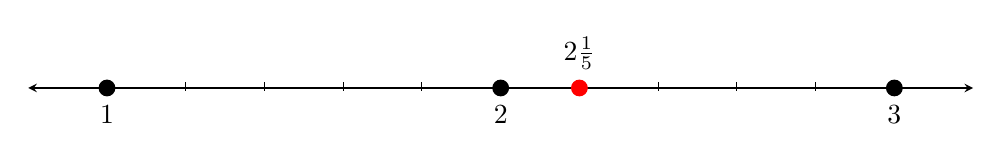
\begin{tikzpicture}
% a straight line segment
\draw [<->] (0,0) -- (12,0);
% the ticks and their labels
\foreach \x  in {1,...,11}
  \draw[xshift=\x cm] (0pt,2pt) -- (0pt,-1pt);
\node[fill=black,draw=black,circle,inner sep=2pt,label=below:{$2$}] at (6,0) {};
\node[fill=black,draw=black,circle,inner sep=2pt,label=below:{$3$}] at (11,0) {};
\node[fill=black,draw=black,circle,inner sep=2pt,label=below:{$1$}] at (1,0) {};
\node[fill=red,draw=red,circle,inner sep=2pt,label=above:{$2\frac{1}{5}$}] at (7,0) {};
\end{tikzpicture}

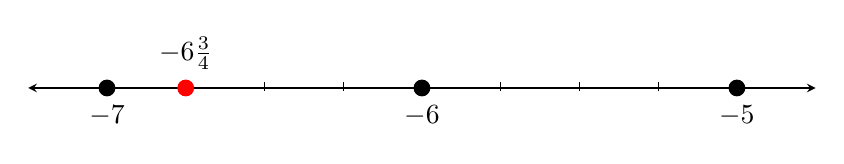
\begin{tikzpicture}
% a straight line segment
\draw [<->] (0,0) -- (10,0);
% the ticks and their labels
\foreach \x  in {1,...,9}
  \draw[xshift=\x cm] (0pt,2pt) -- (0pt,-1pt);
\node[fill=black,draw=black,circle,inner sep=2pt,label=below:{$-6$}] at (5,0) {};
\node[fill=black,draw=black,circle,inner sep=2pt,label=below:{$-5$}] at (9,0) {};
\node[fill=black,draw=black,circle,inner sep=2pt,label=below:{$-7$}] at (1,0) {};
\node[fill=red,draw=red,circle,inner sep=2pt,label=above:{$-6\frac{3}{4}$}] at (2,0) {};
\end{tikzpicture}

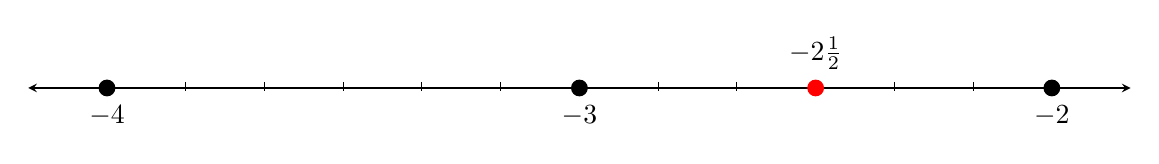
\begin{tikzpicture}
% a straight line segment
\draw [<->] (0,0) -- (14,0);
% the ticks and their labels
\foreach \x  in {1,...,13}
  \draw[xshift=\x cm] (0pt,2pt) -- (0pt,-1pt);
\node[fill=black,draw=black,circle,inner sep=2pt,label=below:{$-4$}] at (1,0) {};
\node[fill=black,draw=black,circle,inner sep=2pt,label=below:{$-3$}] at (7,0) {};
\node[fill=black,draw=black,circle,inner sep=2pt,label=below:{$-2$}] at (13,0) {};
\node[fill=red,draw=red,circle,inner sep=2pt,label=above:{$-2\frac{1}{2}$}] at (10,0) {};
\end{tikzpicture}
\captionof{figure}{Locate mixed numbers on number line}

\end{center}

On the last number line, note that the segment from $-4$ to $-3$ is cut evenly into $6$ pieces, implying each piece represents $\frac{1}{6}$.

The red dot represents $-2\frac{3}{6}$. We must reduce the fraction: $-2\frac{3}{6}=-2\frac{1}{2}$.

\subsection{Summary}
Let's review what we learned in this lesson:
\begin{itemize}
\item To change a mixed number to an improper fraction, we do:
\[ 3\frac{4}{5} = \frac{3\cdot5+4}{5} = \frac{19}{5} \]
\item To change an improper fraction to a mixed number, we first do a division:
\[ 19\div5=3R4 \]
Next we have:
\[ \frac{19}{5}=3\frac{4}{5} \]
Understand that the $3$ represents $3$ whole pies, and the $4$ represents $4$ extra pieces (the remainder).
\end{itemize}



\section{Add/Subtract Mixed Numbers}

In this lesson, we will learn how to add and subtract mixed numbers. We still need the skill of finding common denominators we learned earlier.

\subsection{Add/Subtract a Mixed Number and an Integer}

The following two examples should be easy to understand.

\begin{myexample}
\[ 
\begin{aligned}[t]
	&5\frac{2}{7}+3 = 8\frac{2}{7} \\
	&5\frac{2}{7}-3 = 2\frac{2}{7} \\
\end{aligned}
\]
\end{myexample}

The next example takes some thinking: When we subtract a mixed number like $5\frac{2}{7}$, it's equivalent to first subtracting $5$ whole pies, and then subtracting $\frac{2}{7}$ of a pie. Here are the first few steps of doing $7-5\frac{2}{7}$:

\[ 
\begin{aligned}[t]
	&\phantom{{}=} 7-5\frac{2}{7} \\
	&= 7-5-\frac{2}{7} \\
	&= 2-\frac{2}{7} \\
	&= ...
\end{aligned}
\]

Next, think about the situation: There are $2$ whole pies, and someone ate $\frac{2}{7}$ of one pie. There is still one whole pie left. The other pie, cut into $7$ pieces with $2$ pieces eaten, still has $5$ pieces left. So we have: $2-\frac{2}{7}=1\frac{5}{7}$. The full solution is:
\[ 
\begin{aligned}[t]
	&\phantom{{}=} 7-5\frac{2}{7} \\
	&= 7-5-\frac{2}{7} \\
	&= 2-\frac{2}{7} \\
	&= 1\frac{5}{7}
\end{aligned}
\]

Let's look at another example:
\begin{myexample}
\[ 
\begin{aligned}[t]
	&\phantom{{}=}10-4\frac{9}{20} \\
	&=10-4-\frac{9}{20} \\
	&=6-\frac{9}{20} \\
	&=5\frac{11}{20}
\end{aligned}
\]
\end{myexample}

It's more complicated when negative numbers are involved. See the next two examples.

\begin{myexample}
\[ 
\begin{aligned}[t]
	&\phantom{{}=}4-10\frac{9}{20} \\
	&=4-10-\frac{9}{20} \\
	&=-6-\frac{9}{20} \\
	&=-6\frac{9}{20}
\end{aligned}
\]
If you have trouble understanding the last step, think about $-1-2=-3$ (we need to add $1$ and $2$).
\end{myexample}

\begin{myexample}
\[ 
\begin{aligned}[t]
	&\phantom{{}=}-4-10\frac{9}{20} \\
	&=-4-10-\frac{9}{20} \\
	&=-14-\frac{9}{20} \\
	&=-14\frac{9}{20}
\end{aligned}
\]
\end{myexample}

\subsection{Add/Subtract Mixed Numbers with the Same Denominator}
The key is to break a mixed number into an integer and a fraction. Let's look at a few examples.

\begin{myexample}
\[ 
\begin{aligned}[t]
	&\phantom{{}=}2\frac{1}{6}+3\frac{1}{6} \\
	&= 2+\frac{1}{6}+3+\frac{1}{6} \\
	&= 2+3+\frac{1}{6}+\frac{1}{6} \\
	&= 5+\frac{1+1}{6} \\
	&= 5+\frac{2}{6} \\
	&= 5\frac{1}{3}
\end{aligned}
\]
\end{myexample}

The next example is more complicated.

\begin{myexample}
\[ 
\begin{aligned}[t]
	&\phantom{{}=}2\frac{5}{6}+3\frac{5}{6} \\
	&= 2+\frac{5}{6}+3+\frac{5}{6} \\
	&= 2+3+\frac{5}{6}+\frac{5}{6} \\
	&= 5+\frac{5+5}{6} \\
	&= 5+\frac{10}{6} \\
	&= 5+\frac{5}{3} \\
	&= 5+1\frac{2}{3} \\
	&= 6\frac{2}{3}
\end{aligned}
\]
In this example, we changed $\frac{5}{3}$ to $1\frac{2}{3}$.
\end{myexample}

The next example shows how to do mixed number subtraction. Again, the key is to break the mixed number into an integer and a fraction.

\begin{myexample}
\[ 
\begin{aligned}[t]
	&\phantom{{}=}7\frac{5}{6}-4\frac{1}{6} \\
	&= 7+\frac{5}{6}-4-\frac{1}{6} \\
	&= 7-4+\frac{5}{6}-\frac{1}{6} \\
	&= 3+\frac{5-1}{6} \\
	&= 3+\frac{4}{6} \\
	&= 3\frac{2}{3}
\end{aligned}
\]
\end{myexample}

The next example is more challenging. We need to review how to do subtraction like $31-17$. Once we line up those two numbers, we have:
\[
\begin{aligned}[t]
	&\phantom{-}31 \\
	&\underline{-17}
\end{aligned}
\]

Since we cannot do $1-7$ in the ones place, we use the concept of "borrowing" by taking $10$ from $30$, and put the $10$ to the $1$ in the ones place. Now, the number $31$ is broken into $20$ and $11$.

Now we can do $20-10$ in the tens place, and $11-7$ in the ones place, and the final answer is $14$.

We will use the same concept to do the following mixed number subtraction problem:

\begin{myexample}
\[ 
\begin{aligned}[t]
	&\phantom{{}=}7\frac{1}{6}-4\frac{5}{6} \\
	&= 7+\frac{1}{6}-4-\frac{5}{6} \\
	&= 7-4+\frac{1}{6}-\frac{5}{6} \\
	&= 3+\frac{1}{6}-\frac{5}{6} \\
	&= 2+1+\frac{1}{6}-\frac{5}{6} & \text{borrowing 1 from 3}\\
	&= 2+\frac{6}{6}+\frac{1}{6}-\frac{5}{6} &\text{change }1\text{ to } \frac{6}{6}\\
	&= 2+\frac{7}{6}-\frac{5}{6} \\
	&= 2+\frac{2}{6} \\
	&= 2\frac{1}{3} &\text{reduce fraction} \\
\end{aligned}
\]
In this example, since we cannot subtract $\frac{5}{6}$ from $\frac{1}{6}$, we "borrowed" $1$ from the integer $3$, changed $1$ to $\frac{6}{6}$, and then changed $\frac{1}{6}$ to $\frac{6}{6}+\frac{1}{6}=\frac{7}{6}$. Now we can subtract $\frac{5}{6}$ from $\frac{7}{6}$. This is the same strategy we used when we do $31-17=14$.
\end{myexample}

Things become more complicated when negative numbers are involved. See the next few examples.

\begin{myexample}
\[ 
\begin{aligned}[t]
	&\phantom{{}=}-7\frac{1}{6}-4\frac{5}{6} \\
	&= -7-\frac{1}{6}-4-\frac{5}{6} \\
	&= -7-4-\frac{1}{6}-\frac{5}{6} \\
	&= -11+(-\frac{1}{6})+(-\frac{5}{6}) \\
	&= -11+\frac{(-1)+(-5)}{6} \\
	&= -11+\frac{-6}{6} \\
	&= -11+(-1) \\
	&= -12
\end{aligned}
\]
To make it clear, we changed $-\frac{1}{6}-\frac{5}{6}$ to $(-\frac{1}{6})+(-\frac{5}{6})$. This is like changing $-1-2$ to $(-1)+(-2)$.
\end{myexample}

\begin{myexample}
\[ 
\begin{aligned}[t]
	&\phantom{{}=}-7\frac{5}{6}+4\frac{1}{6} \\
	&= -7-\frac{5}{6}+4+\frac{1}{6} \\
	&= -7+4-\frac{5}{6}+\frac{1}{6} \\
	&= -3+\frac{-5}{6}+\frac{1}{6} \\
	&= -3+\frac{-5+1}{6} \\
	&= -3+\frac{-4}{6} \\
	&= -3+\frac{-2}{3} \\
	&= -3\frac{2}{3}
\end{aligned}
\]
The last step takes some thinking. Think of $(-1)+(-2)=-3$. When we add two negative numbers, we actually add up the absolute value of those two numbers. This is why when we do $-3+\frac{-2}{3}$, we need to do $3+\frac{2}{3}=3\frac{2}{3}$, and then make it negative.
\end{myexample}

\begin{myexample}
\[ 
\begin{aligned}[t]
	&\phantom{{}=}1\frac{5}{6}-4 \\
	&= 1+\frac{5}{6}-4 \\
	&= 1-4+\frac{5}{6} \\
	&= -3+\frac{5}{6} \\
	&= -2 -1 + \frac{5}{6} \\
	&= -2 -\frac{6}{6} + \frac{5}{6} \\
	&= -2 + \frac{-6+5}{6} \\
	&= -2 + \frac{-1}{6} \\
	&= -2\frac{1}{6}
\end{aligned}
\]
\end{myexample}

Adding/subtracting mixed numbers with different denominators is more complicated, but the strategies are the same.

\subsection{Summary}
When we do mixed number addition/subtraction, we usually break up the mixed number into its integer part and fraction part. For example:
\[ 2\frac{3}{5} = 2+\frac{3}{5} \]
\[ -2\frac{3}{5} = -2-\frac{3}{5} \]

A lot of practice is needed for mixed number addition/subtraction. Make sure you understand each step as you go.



\section{Multiply/Divide Mixed Numbers}

In this lesson, we will learn how to multiply and divide mixed numbers. The rule is very simply: Before we multiply/divide mixed numbers, we need to change them (like $1\frac{1}{2}$) to improper fractions (like $\frac{3}{2}$), and then use fraction multiplication/division rules we learned earlier.

\subsection{Multiply/Divide Mixed Numbers}

You might need to go back to review how to change a mixed number to an improper fraction.

\begin{myexample}
\[ 
\begin{aligned}[t]
	&\phantom{{}=} 1\frac{1}{2} \cdot 3\frac{5}{6} \\
	&= \frac{3}{2} \cdot \frac{23}{6} \\
	&= \frac{3\div3}{2} \cdot \frac{23}{6\div3} \\
	&= \frac{1}{2} \cdot \frac{23}{2} \\
	&= \frac{1\cdot23}{2\cdot2} \\
	&= \frac{23}{4} \\
	&= 5\frac{3}{4}
\end{aligned}
\]
The last step is optional, depending on what the question asks. If the question doesn't ask for a mixed number answer, you could leave the answer as $\frac{23}{4}$.
\end{myexample}

\begin{myexample}
\[ 
\begin{aligned}[t]
	&\phantom{{}=} 8\frac{1}{4} \div 3 \\
	&= \frac{33}{4} \div \frac{3}{1} \\
	&= \frac{33}{4} \cdot \frac{1}{3} \\
	&= \frac{33\div3}{4} \cdot \frac{1}{3\div3} \\
	&= \frac{11}{4} \cdot \frac{1}{1} \\
	&= \frac{11}{4} \\
	&= 2\frac{3}{4}
\end{aligned}
\]
\end{myexample}

\subsection{Word Problems}

\begin{myexample}
Each truck can hold $3\frac{1}{4}$ tons of sand. In a job, it took $24$ full truck loads to transfer a certain amount of sand. How many tons of sand were transferred?
\end{myexample}
\begin{solution}
This is obviously a multiplication problem:
\[ 
\begin{aligned}[t]
	&\phantom{{}=} 3\frac{1}{4} \cdot 24 \\
	&= \frac{13}{4} \cdot \frac{24}{1} \\
	&= \frac{13}{4\div4} \cdot \frac{24\div4}{1} \\
	&= \frac{13}{1} \cdot \frac{6}{1} \\
	&= \frac{13\cdot6}{1\cdot1} \\
	&= \frac{78}{1} \\
	&= 78
\end{aligned}
\]
\textbf{Conclusion:} Those trucks transferred $78$ tons of sand.
\end{solution}


\begin{myexample}
In a running contest (with breaks), each runner will run $28$ miles. A runner runs $5\frac{1}{4}$ miles per hour. How many hours will it take the runner to complete the race?
\end{myexample}
\begin{solution}
In this problem, we need to find out how many $5\frac{1}{4}$ miles are in $28$ miles, a division problem:
\[ 
\begin{aligned}[t]
	&\phantom{{}=} 28 \div 5\frac{1}{4} \\
	&= \frac{28}{1} \div \frac{21}{4} \\
	&= \frac{28}{1} \cdot \frac{4}{21} \\
	&= \frac{28\div7}{1} \cdot \frac{4}{21\div7} \\
	&= \frac{4}{1} \cdot \frac{4}{3} \\
	&= \frac{16}{3} \\
	&= 5\frac{1}{3}
\end{aligned}
\]

\textbf{Conclusion:} It would take the runner $5\frac{1}{3}$ hours to complete the race. 

Since each hour has $60$ minutes, $\frac{1}{3}$ of an hour has $20$ minutes, so it would take the runner $5$ hours and $20$ minutes to complete the race.

In this problem, it would not be good to say it would take the runner $\frac{16}{3}$ hours to complete the race.
\end{solution}

\begin{myexample}
Find the area of the following rectangle.
\begin{center}
\begin{tikzpicture}
	\draw (0,0) rectangle (4,3);
	\draw(2,-0.5) node{$2\frac{1}{4}$ in};
	\draw(-0.5,1.5) node{$1\frac{2}{3}$ in};
\end{tikzpicture}
\captionof{figure}{Find the area of the rectangle}
\end{center}
\end{myexample}
\begin{solution}
To find the area of a rectangle, we multiply the base and the height:
\[ 
\begin{aligned}[t]
	&\phantom{{}=} 2\frac{1}{4} \cdot 1\frac{2}{3} \\
	&= \frac{9}{4} \cdot \frac{5}{3} \\
	&= \frac{9\div3}{4} \cdot \frac{5}{3\div3} \\
	&= \frac{3}{4} \cdot \frac{5}{1} \\
	&= \frac{15}{4} \\
	&= 3\frac{3}{4}
\end{aligned}
\]
\textbf{Conclusion:} The area of the rectangle is $3\frac{3}{4}$ square inches (or $\text{in}^{2}$).
\end{solution}

\begin{myexample}
Find the area of the following triangle.
\begin{center}
\begin{tikzpicture}
	\draw (0,0) -- (4,0) -- (0,3) -- (0,0);
	\draw (0,0.2) -- (0.2,0.2) -- (0.2,0);
	\draw(2,-0.5) node{$2\frac{1}{4}$ in};
	\draw(-0.5,1.5) node{$1\frac{2}{3}$ in};
\end{tikzpicture}
\captionof{figure}{Find the area of the triangle}
\end{center}
\end{myexample}
\begin{solution}

Notice that a triangle is actually half a rectangle. See the following figure:
\begin{center}
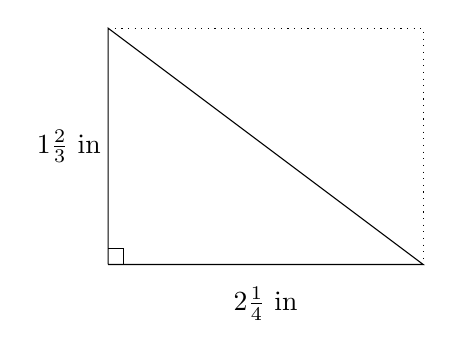
\begin{tikzpicture}
	\draw (0,0) -- (4,0) -- (0,3) -- (0,0);
	\draw (0,0.2) -- (0.2,0.2) -- (0.2,0);
	\draw[dotted] (0,3) -- (4,3) -- (4,0);
	\draw(2,-0.5) node{$2\frac{1}{4}$ in};
	\draw(-0.5,1.5) node{$1\frac{2}{3}$ in};
\end{tikzpicture}
\captionof{figure}{A triangle is half of a rectangle}
\label{fig:MultiplyDivideMixedNumbers1}
\end{center}

To find the area of a triangle, we use the following formula:
\[ \text{triangle area}=(\text{base})(\text{height})\div2 \]
Now that we learned fraction, we could re-write the formula as:
\[ \text{triangle area}=\frac{1}{2}(\text{base})(\text{height}) \]
We find a rectangle's area by multiplying the base and the height. In the formula to find a triangle's area, the $\frac{1}{2}$ is there because a triangle's area is half of a rectangle, by \cref{fig:MultiplyDivideMixedNumbers1}.

Now we have:
\[ 
\begin{aligned}[t]
	\text{area}&= \frac{1}{2} \cdot 2\frac{1}{4} \cdot 1\frac{2}{3} \\
	&= \frac{1}{2} \cdot \frac{9}{4} \cdot \frac{5}{3} \\
	&= \frac{1}{2} \cdot \frac{9\div3}{4} \cdot \frac{5}{3\div3} \\
	&= \frac{1}{2} \cdot \frac{3}{4} \cdot \frac{5}{1} \\
	&= \frac{15}{8} \\
	&= 1\frac{7}{8}
\end{aligned}
\]

\textbf{Conclusion:} The area of the rectangle is $1\frac{7}{8}$ square inches (or $\text{in}^{2}$).
\end{solution}



\section{Order of Operations involving Fractions}

In this lesson, we will do a few order-of-operations problems involving fractions.

We have learned the order of operations in earlier lessons:

\[
\begin{aligned}[t]
   &P &\text{(Parentheses)} \\
   &E &\text{(Exponent)} \\
   &MD &\text{(Multiplication and Division)} \\
   &AS &\text{(Addition and Subtraction)}
\end{aligned}
\]
\captionof{figure}{Order of Operations}
\label{fig:PEMDAS38}

In this lesson, the rules didn't change, except fractions are involved. We will simply look at a few examples.

\begin{myexample}
\[
\begin{aligned}[t]
	&\phantom{{}=} \frac{5}{4}+(\frac{3}{4})2 \\
	&= \frac{5}{4}+\frac{3}{4} \cdot \frac{2}{1} \\
	&= \frac{5}{4}+\frac{3}{4\div2} \cdot \frac{2\div2}{1} \\
	&= \frac{5}{4}+\frac{3}{2} \cdot \frac{1}{1} \\
   	&= \frac{5}{4}+\frac{3}{2} \\
   	&= \frac{5}{4}+\frac{3\cdot2}{2\cdot2} \\
   	&= \frac{5}{4}+\frac{6}{4} \\
	&= \frac{11}{4}
\end{aligned}
\]
Without specified instruction, there is no need to change $\frac{11}{4}$ into $3\frac{3}{4}$.
\end{myexample}

\begin{myexample}
\[
\begin{aligned}[t]
	&\phantom{{}=} \frac{4}{3}-5(\frac{1}{9}-\frac{1}{6}) \\
	&= \frac{4}{3}-5(\frac{1\cdot2}{9\cdot2}-\frac{1\cdot3}{6\cdot3}) \\
	&= \frac{4}{3}-5(\frac{2}{18}-\frac{3}{18}) \\
	&= \frac{4}{3}-5(-\frac{1}{18}) \\
	&= \frac{4}{3}+5(\frac{1}{18}) &(\text{negative})\cdot(\text{negative})=\text{positive}\\
	&= \frac{4}{3}+\frac{5}{1} \cdot \frac{1}{18} \\
	&= \frac{4}{3}+\frac{5}{18} \\
	&= \frac{4\cdot6}{3\cdot6}+\frac{5}{18} \\
	&= \frac{24}{18}+\frac{5}{18} \\
	&= \frac{29}{18}
\end{aligned}
\]
In the step 
\[ \frac{4}{3}-5(-\frac{1}{18}) \] 
we treat the subtraction symbol as a negative symbol, so we have 
\[ \frac{4}{3}+(-5)\cdot(-\frac{1}{18}) \]
Since $(\text{negative})\cdot(\text{negative})=\text{positive}$, we have 
\[ \frac{4}{3}+(-5)\cdot(-\frac{1}{18})=\frac{4}{3}+5(\frac{1}{18}) \]
\end{myexample}

\begin{myexample}
Compare the following example with the last one, and see the difference between parentheses and absolute value.

\[
\begin{aligned}[t]
	&\phantom{{}=} \frac{4}{3}-5 \left| \frac{1}{9}-\frac{1}{6} \right| \\
	&= \frac{4}{3}-5 \left| \frac{1\cdot2}{9\cdot2}-\frac{1\cdot3}{6\cdot3} \right| \\
	&= \frac{4}{3}-5 \left| \frac{2}{18}-\frac{3}{18} \right| \\
	&= \frac{4}{3}-5 \left| -\frac{1}{18} \right| \\
	&= \frac{4}{3}-5(\frac{1}{18}) \\
	&= \frac{4}{3}-\frac{5}{1} \cdot \frac{1}{18} \\
	&= \frac{4}{3}-\frac{5}{18} \\
	&= \frac{4\cdot6}{3\cdot6}-\frac{5}{18} \\
	&= \frac{24}{18}-\frac{5}{18} \\
	&= \frac{19}{18}
\end{aligned}
\]
\end{myexample}

\begin{myexample}
Compare these two examples:

\begin{tabular}[t]{c@{\hspace{4cm}}c@{\hspace{2cm}}c}
&
$ \begin{aligned}[t] 
	&\phantom{{}=} 1-(\frac{2}{3})^{2} \\ 
	&= 1-(\frac{2}{3})(\frac{2}{3}) \\ 
	&= 1-\frac{2\cdot2}{3\cdot3} \\
	&= 1-\frac{4}{9} \\
	&= \frac{9}{9}-\frac{4}{9} \\
	&= \frac{5}{9}
  \end{aligned} $ 
&
$ \begin{aligned}[t] 
	&\phantom{{}=} 1-(-\frac{2}{3})^{2} \\ 
	&= 1-(-\frac{2}{3})(-\frac{2}{3}) \\ 
	&= 1-(\frac{2}{3})(\frac{2}{3}) \\ 
	&= 1-\frac{2\cdot2}{3\cdot3} \\
	&= 1-\frac{4}{9} \\
	&= \frac{9}{9}-\frac{4}{9} \\
	&= \frac{5}{9}
  \end{aligned} $ 
\end{tabular}

Note that $(\frac{2}{3})^{2}=\frac{4}{9}$, and $(-\frac{2}{3})^{2}=\frac{4}{9}$.
\end{myexample}

\begin{myexample}
Compare these two examples:

\begin{tabular}[t]{c@{\hspace{4cm}}c@{\hspace{2cm}}c}
&
$ \begin{aligned}[t] 
	&\phantom{{}=} 1-(\frac{2}{3})^{3} \\ 
	&= 1-(\frac{2}{3})(\frac{2}{3})(\frac{2}{3}) \\ 
	&= 1-\frac{2\cdot2\cdot2}{3\cdot3\cdot3} \\
	&= 1-\frac{8}{27} \\
	&= \frac{27}{27}-\frac{8}{27} \\
	&= \frac{19}{27}
  \end{aligned} $ 
&
$ \begin{aligned}[t] 
	&\phantom{{}=} 1-(-\frac{2}{3})^{3} \\ 
	&= 1-(-\frac{2}{3})(-\frac{2}{3})(-\frac{2}{3}) \\ 
	&= 1+(\frac{2}{3})(\frac{2}{3})(\frac{2}{3}) \\ 
	&= 1+\frac{2\cdot2\cdot2}{3\cdot3\cdot3} \\
	&= 1+\frac{8}{27} \\
	&= \frac{27}{27}+\frac{8}{27} \\
	&= \frac{35}{27}
  \end{aligned} $ 
\end{tabular}

Note that $1-(-\frac{2}{3})(-\frac{2}{3})(-\frac{2}{3})$ becomes $1+(\frac{2}{3})(\frac{2}{3})(\frac{2}{3})$ because each pair of negative symbols canceled each other.

Compare $(\frac{2}{3})^{3}=\frac{8}{27}$ and $(-\frac{2}{3})^{3}=-\frac{8}{27}$.

Earlier, we learned: $(\frac{2}{3})^{2}=\frac{4}{9}$, and $(-\frac{2}{3})^{2}=\frac{4}{9}$.

Instead of trying to memorize these results, understand that each pair of negative symbols cancel each other (in multiplication).
\end{myexample}




\chapter{Decimals}
\section{Introduction to Decimals}
\thispagestyle{fancy}

We use decimals every day as we buy things. For example, each pound of apple costs \$$1.99$. In this lesson, we will learn the definition of decimals.

\subsection{Definition of Decimals}
The best way to understand decimals is to think of money, because we deal with money every day. For example, $1.99$ means $1$ dollar and $99$ cents.

\subsection{Types of Decimals}
There are a few types of decimals:
\begin{itemize}
\item \textbf{terminating decimal}: A terminating decimal has a limited number of places, like $0.1,1.23,1.2345$.
\item \textbf{repeating decimal}: A repeating decimal goes on forever repeating the same digits again and again, like $0.111...,4.121212...,5.3124124124...$. A repeating decimal can be re-written with a bar over the repeating digits:
\[
\begin{aligned}[t]
	0.111... &= 0.\overline{1} \\
	4.121212... &= 0.\overline{12} \\
	5.3124124124... &= 5.3\overline{124} 
\end{aligned}
\]
\item \textbf{irrational decimal}: An irrational decimal goes on forever without repeating any pattern. Here are a few examples:
\[
\begin{aligned}[t]
	\pi &= 3.1415926... \\
	\sqrt{2} &= 1.414... \\
	\sqrt{3} &= 1.732...
\end{aligned}
\]
\end{itemize}

\subsubsection{The decimal $0.03$}
Think of the number $0.03$, which is $3$ cents. Since each dollar has $100$ cents, $0.03$ represents $3$ out of $100$, or, in fraction, $\frac{3}{100}$. This fraction is read as "three hundredths".

This is why we call the second digit after the decimal point the \textit{hundredths place.} We could read $0.03$ either as "three hundredths," or simply "zero point zero three."

Here is one way to represent $0.03$ graphically (the grid has $100$ cells):

\begin{center}
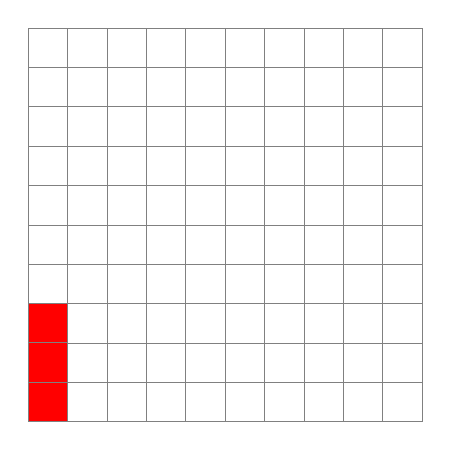
\begin{tikzpicture}
	\draw[step=0.5cm,gray,very thin] (0,0) grid (5,5);
	\filldraw[fill=red, draw=gray] (0,0) rectangle (0.5,0.5);
	\filldraw[fill=red, draw=gray] (0,0.5) rectangle (0.5,1);
	\filldraw[fill=red, draw=gray] (0,1) rectangle (0.5,1.5);
\end{tikzpicture}
\captionof{figure}{Graphic representation of $0.03$}
\end{center}

\subsubsection{The decimal $0.3$}
Let's look at another number: $0.3$. This number does not represent $3$ cents, because earlier we learned $0.03$ represents $3$ cents. The difference is that, in $0.3$, the number $3$ is in the tenths place. In terms of money, $0.3$ represents $30$ cents. On a price mark, we usually write $0.3$ as \$$0.30$. This revealed an important property of decimals:

\textbf{If we add the digit $0$ to the end of a decimal (behind the decimal point), the decimal's value doesn't change.} For example: $0.30=0.3$, $0.300=0.3$, $1.20=1.2$.

Note that $1.3\neq1.03$: the number $1.3$ represents a dollar and $30$ cents, while the number $1.03$ represents a dollar and $3$ cents.

The number $0.3$ represents $3$ out of $10$, or, in fraction, $\frac{3}{10}$. This fraction is read as "three tenths".

This is why we call the digit after the decimal point the \textit{tenths place.} We could read $0.3$ either as "three tenths," or simply "zero point three."

Here is one way to represent $0.3$ graphically:

\begin{center}
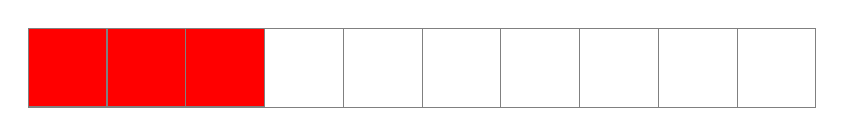
\begin{tikzpicture}
	\draw[step=1cm,gray,very thin] (0,0) grid (10,1);
	\filldraw[fill=red, draw=gray] (0,0) rectangle (1,1);
	\filldraw[fill=red, draw=gray] (1,0) rectangle (2,1);
	\filldraw[fill=red, draw=gray] (2,0) rectangle (3,1);
\end{tikzpicture}
\captionof{figure}{Graphic representation of $0.3$}
\end{center}

\subsubsection{The decimal $0.003$}
Finally, let's look at $0.003$. Earlier, we learned that $0.03$ represents $3$ cents. The number $0.003$ is three tenth of a cent. If you look carefully at gas price next time you fill up, each gallon actually costs something like \$$3.159$. Notice the last digit is always $9$. Nine tenths of a cent is not a lot of money, but the profit adds up.

The number $0.003$ represents $3$ out of $1000$, or, in fraction, $\frac{3}{1000}$. This fraction is read as "three thousandths".

This is why we call the third digit after the decimal point the \textit{thousandths place.} We could read $0.003$ either as "three thousandths," or simply "zero point zero zero three."

We will not represent $0.003$ graphically here, because it's hard to draw a grid with $1,000$ cells.

\subsection{Read Decimals}
For the decimal $1,234.5678$, here are the names of each digit:
\begin{itemize}
\item $1$ is in the thousands place, representing one thousand.
\item $2$ is in the hundreds place, representing two hundred.
\item $3$ is in the tens place, representing thirty.
\item $4$ is in the ones place, representing four.
\item $5$ is in the tenths place, representing five tenths ($50$ cents).
\item $6$ is in the hundredths place, representing six hundredths ($6$ cents).
\item $7$ is in the thousandths place, representing seven thousandths.
\item $8$ is in the ten-thousandths place, representing eight ten-thousandths.
\end{itemize}

Here are a few examples of how to read decimals:

\begin{itemize}
\item $12.3$ reads: twelve and three tenths
\item $12.34$ reads: twelve and thirty four hundredths
\item $12.345$ reads: twelve and three hundred forty-five thousandths
\item $12.3456$ reads: twelve and three thousand four hundred fifty-six ten-thousandths
\item $12.03$ reads: twelve and three hundredths
\item $12.003$ reads: twelve and three thousandths
\end{itemize}

\subsection{Decimals on Number Line}
Here are a few examples on how to locate decimals on the number line:

\begin{center} 
\begin{tikzpicture}
% a straight line segment
\draw [<->] (0,0) -- (12,0);
% the ticks and their labels
\foreach \x  in {1,...,11}
  \draw[xshift=\x cm] (0pt,2pt) -- (0pt,-1pt);
\node[fill=black,draw=black,circle,inner sep=2pt,label=below:{$0$}] at (1,0) {};
\node[fill=black,draw=black,circle,inner sep=2pt,label=below:{$1$}] at (11,0) {};
\node[fill=red,draw=red,circle,inner sep=2pt,label=above:{$0.3$}] at (4,0) {};
\end{tikzpicture}

\begin{tikzpicture}
% a straight line segment
\draw [<->] (0,0) -- (12,0);
% the ticks and their labels
\foreach \x  in {1,...,11}
  \draw[xshift=\x cm] (0pt,2pt) -- (0pt,-1pt);
\node[fill=black,draw=black,circle,inner sep=2pt,label=below:{$-3$}] at (1,0) {};
\node[fill=black,draw=black,circle,inner sep=2pt,label=below:{$-2$}] at (11,0) {};
\node[fill=red,draw=red,circle,inner sep=2pt,label=above:{$-2.7$}] at (4,0) {};
\end{tikzpicture}

\begin{tikzpicture}
% a straight line segment
\draw [<->] (0,0) -- (12,0);
% the ticks and their labels
\foreach \x  in {1,...,11}
  \draw[xshift=\x cm] (0pt,2pt) -- (0pt,-1pt);
\node[fill=black,draw=black,circle,inner sep=2pt,label=below:{$-3.1$}] at (1,0) {};
\node[fill=black,draw=black,circle,inner sep=2pt,label=below:{$-3$}] at (11,0) {};
\node[fill=red,draw=red,circle,inner sep=2pt,label=above:{$-3.07$}] at (4,0) {};
\end{tikzpicture}
\captionof{figure}{Decimals on the number line}
\end{center}

\subsection{Compare Decimals}
Which one is bigger, $3.09$ or $3.81$? It's easy to compare if we think about money: three dollars and eighty-one cents is bigger than three dollars and nine cents. So we have:
\[ 3.09<3.81 \]

So, when we compare decimals, we compare the tenths' place first, and then the hundredths' place. Even though the digit $9$ in $3.09$ is bigger than $8$ in $3.81$, the number $3.81$ is bigger than $3.09$.

We have the following comparisons:
\[
\begin{aligned}[t]
	1.29 &< 1.30 \\
	4.29 &> 1.30 \\
	3.04 &< 3.4 \\
	0.031 &> 0.009 
\end{aligned}
\]
Comparing negative numbers is "opposite:"
\[
\begin{aligned}[t]
	-1.29 &> -1.30 \\
	-4.29 &< -1.30 \\
	-3.04 &> -3.4 \\
	-0.031 &< -0.009 
\end{aligned}
\]
Finally, be careful when there are trailing zeroes:
\[
\begin{aligned}[t]
	1.10 &= 1.1 \\
	0.03 &= 0.030 \\
	-0.300 &= -0.3 
\end{aligned}
\]

\subsection{Round Decimals}
Earlier, we learned how to round whole numbers. The concept of rounding decimals is the same. For example, to round $1.19$ to an integer, we have $1.19\approx1$ because $1.19$ is closer to $1$ than $2$. Let's look at a few examples:

\begin{myexample}
Round $1.295$ to the tenths place.
\end{myexample}
\begin{solution}
In $1.295$, the tenths place is $2$. The digit behind it is $9$. Since $9$ is bigger than $4$, we round up:
\[ 1.295 \approx 1.3 \]
\end{solution}

\begin{myexample}
Round $1.245$ to the tenths place.
\end{myexample}
\begin{solution}
In $1.245$, the tenths place is $2$. The digit behind it is $4$. Since $4$ is smaller than $5$, we don't round up:
\[ 1.245 \approx 1.2 \]
\end{solution}

\begin{myexample}
Round $1.295$ to the hundredths place.
\end{myexample}
\begin{solution}
In $1.295$, the hundredths place is $9$. The digit behind it is $5$. Since $5$ is bigger than $4$, we round up:
\[ 1.295 \approx 1.30 \]
\end{solution}



\section{Add/Subtract Decimals}

In this section, we will learn how to add/subtract decimals. 

Although we could use calculator to do decimal calculations, it's important to understand the theory and do some calculations without using calculator. Please refrain from using calculator in this section (actually in this whole course).

In most cases, we add/subtract decimals in the "normal" way.

\begin{tabular}[t]{c@{\hspace{4cm}}c@{\hspace{2cm}}c}
&
$ \begin{aligned}[t] 
	&\phantom{+}12.34 \\
	&\underline{+23.45} \\
	&\phantom{+}35.79
  \end{aligned} $ 
&
$ \begin{aligned}[t] 
	&\phantom{-}98.76 \\
	&\underline{-23.45} \\
	&\phantom{-}75.31
  \end{aligned} $ 
\end{tabular}

However, it takes some thinking to do $0.2+0.03$. A common mistake is to do $0.2+0.03=0.5$. Let's think about money.

The number $0.2$ means $20$ cents; the number $0.03$ means $3$ cents; so $0.2+0.03$ should be $23$ cents, or $0.2+0.03=0.23$. Here is how we should line up $0.2$ and $0.03$:

\[
\begin{aligned}[t] 
	&\phantom{+}0.2 \\
	&\underline{+0.03} \\
	&\phantom{+}0.23
\end{aligned}
\]

Here is the rule: When we add/subtract decimals, we must line up the decimal point.

When we subtract decimals, sometimes we need to fill in some zeros at the end. For example, when we calculate $0.2-0.03$, we do:

\[
\begin{aligned}[t] 
	&\phantom{-}0.20 \\
	&\underline{-0.03} \\
	&\phantom{-}0.17
\end{aligned}
\]

This result makes sense, as $20$ cents minus $3$ cents is $17$ cents.

For integers like $2$, the decimal point is at the end, even though we don't write it. When we do $2+1.4$, we first change $2$ to $2.0$, and then line up:

\[
\begin{aligned}[t] 
	&\phantom{+}2.0 \\
	&\underline{+1.4} \\
	&\phantom{+}3.4
\end{aligned}
\]

When we do $2-0.04$, we change $2$ to $2.00$, and then line up:

\[
\begin{aligned}[t] 
	&\phantom{-}2.00 \\
	&\underline{-0.04} \\
	&\phantom{-}1.96
\end{aligned}
\]

It's more complicated when negative decimals are involved. We will do two problems with the "money model" (instead of the "number line" model):

\begin{myexample}
Calculate $1.907-2.3$
\end{myexample}
\begin{solution}
\begin{enumerate}
\item Change $1.907-2.3$ to $1.907+(-2.3)$.
\item The first number is 1.907. For the money model, in the first game, I won \$$1.907$.
\item The second number is $-2.3$. For the money model, in the second game, I lost \$$2.3$.
\item Since I lost more money than I won, altogether, I lost some money. This implies the answer must be negative.
\item Since I won some and then lost some, we need to find the difference of $1.907$ and $2.3$. We do:
\[
\begin{aligned}[t] 
	&\phantom{-}2.300 \\
	&\underline{-1.907} \\
	&\phantom{-}0.393
\end{aligned}
\]
\item[6.] Finally, the solution is: $1.907-2.3=-0.393$
\end{enumerate}
\end{solution}

\begin{myexample}
Calculate $-1.907-2.3$
\end{myexample}
\begin{solution}
\begin{enumerate}
\item Change $-1.907-2.3$ to $(-1.907)+(-2.3)$.
\item The first number is $-1.907$. For the money model, in the first game, I lost \$$1.907$.
\item The second number is $-2.3$. For the money model, in the second game, I lost \$$2.3$.
\item Since I lost in both games, altogether, I lost money. This implies the answer must be negative.
\item Since I lost in both games, we need to find the sum of $1.907$ and $2.3$. We do:
\[
\begin{aligned}[t] 
	&\phantom{+}2.300 \\
	&\underline{+1.907} \\
	&\phantom{+}4.207
\end{aligned}
\]
\item[6.] Finally, the solution is: $-1.907-2.3=-4.207$
\end{enumerate}
\end{solution}



\section{Multiply/Divide Decimals}

In this lesson, we will learn how to multiply/divide decimals. Again, please refrain from using calculator in this section (actually in this whole course).

\subsection{Multiply/Divide by Power of 10}
Recall that for the number $12$, we could write it as $12.0$, $12.00$ or $12.000$, as the value doesn't change.

Let's observe a pattern. In the following numbers, I added trailing zeroes and decimal point to the end of integers in order to find the pattern:
\[
\begin{aligned}[t]
	12.0\cdot10 &= 120. \\
	12.00\cdot100 &= 1200. \\
	12.000\cdot1000 &= 12000. \\
\end{aligned}
\]

Here is the pattern: \textbf{When we multiply a number by a power of $10$, like $10,100,1000$..., we move the decimal point to the right as many times as the number of zeroes.}

A similar pattern exists for division:
\[
\begin{aligned}[t]
	12000.\div10 &= 1200. \\
	12000.\div100 &= 120. \\
	12000.\div1000 &= 12. \\
\end{aligned}
\]

Here is the pattern: \textbf{When we divide a number by a power of $10$, like $10,100,1000$..., we move the decimal point to the left as many times as the number of zeroes.}

Don't try to memorize the patterns without understanding. If you forget in which direction the decimal point will move, on scratch paper, do $12.\cdot10=120.$ and $120.\div10=12.$, and then you can quickly recall the patterns.

The same patterns work for decimals. Here are a few examples:
\[
\begin{aligned}[t]
	123.456\cdot10 &= 1234.56 &&\text{Decimal point moves to the right once.}\\
	123.456\cdot100 &= 12345.6 &&\text{Decimal point moves to the right twice.}\\
	123.456\div10 &= 12.3456 &&\text{Decimal point moves to the left once.}\\
	123.456\div100 &= 1.23456 &&\text{Decimal point moves to the left twice.}
\end{aligned}
\]

Sometimes we need to fill in zeroes:
\[
\begin{aligned}[t]
	1.2\cdot100 &= 120 &&\text{Decimal point moves to the right twice.}\\
	1.2\cdot1000 &= 1200 &&\text{Decimal point moves to the right three times.}\\
	1.2\div10 &= 0.12 &&\text{Decimal point moves to the left once.}\\
	1.2\div100 &= 0.012 &&\text{Decimal point moves to the left twice.}\\
	1.2\div1000 &= 0.0012 &&\text{Decimal point moves to the left three times.}\\
\end{aligned}
\]

\subsection{Moving Decimal Point in Multiplication}
It's given that $12\cdot12=144$. What's the product of $12\cdot1.2$?

From the pattern we learned earlier, we know $1.2=12\div10$. So we have:
\[ 
\begin{aligned}[t]
	&\phantom{{}=}12\cdot1.2 \\
	&=12\cdot12\div10 \\
	&=144\div10 \\
	&=14.4
\end{aligned}
\]

Without giving details, with the same method, we can calculate:
\[ 
\begin{aligned}[t]
	12\cdot0.12 &= 1.44 \\
	12\cdot0.012 &= 0.144 \\
	1.2\cdot1.2 &= 1.44 \\
	0.12\cdot12 &= 1.44 \\
	0.12\cdot1.2 &= 0.144
\end{aligned}
\]

Instead of writing a long sentence to summarize the pattern, I will simply use an example. It's given $12\cdot12=144$. When we calculate $0.12\cdot1.2$, observe that the decimal point moved to the left for a total of three times, compared with $12\cdot12$. So, we need to move the decimal point of $144$ to the left three times, and we have $0.12\cdot1.2=0.144$.

The pattern can be applied when we move the decimal point to the left or right. Let's look at a few examples.

\begin{myexample}
Given $123\cdot45=5535$, calculate $1.23\cdot45000$.
\end{myexample}
\begin{solution}
\begin{itemize}
\item From $123$ to $1.23$, the decimal point moved to the left twice.
\item From $45$ to $45000$, the decimal point moved to the right three times.
\item Altogether, the decimal point moved to the right once.
\item We move $5535$'s decimal point to the right once, and we have: $1.23\cdot45000=55350$.
\end{itemize}
\end{solution}

\begin{myexample}
Given $123\cdot45=5535$, calculate $1.23\cdot4500$.
\end{myexample}
\begin{solution}
\begin{itemize}
\item From $123$ to $1.23$, the decimal point moved to the left twice.
\item From $45$ to $4500$, the decimal point moved to the right twice.
\item Altogether, the decimal point didn't move.
\item The decimal point of the product $5535$ didn't move, and we have: $1.23\cdot4500=5535$.
\end{itemize}
\end{solution}

\subsection{Moving Decimal Point in Division}
There are similar rules of moving the decimal point when we do divisions. Let me explain the rules with fractions.

Recall that for a fraction, if we multiply or divide the same number in both the numerator and denominator, the fraction's value doesn't change. For example:
\[ \frac{1}{2}=\frac{1\cdot2}{2\cdot2}=\frac{2}{4} \]
\[ \frac{2}{4}=\frac{2\div2}{4\div2}=\frac{1}{2} \]

Similarly, we have:
\[ \frac{120}{20}=\frac{120\cdot10}{20\cdot10}=\frac{1200}{200} \]
\[ \frac{120}{20}=\frac{120\div10}{20\div10}=\frac{12}{2} \]

Since the fraction line is the same as the division symbol, we can rewrite our observation as:
\[ 120\div20=1200\div200 \]
\[ 120\div20=12\div2 \]

The rule is: \textbf{In a division, if we move the decimal point in both numbers to the same direction for the same number of times, the quotient doesn't change.} For example:
\[
\begin{aligned}[t]
	1.23 \div 0.3 &= 12.3 \div 3 &&\text{Decimal point in both numbers moved to the right once.} \\
	1.23 \div 0.3 &= 123 \div 30 &&\text{Decimal point in both numbers moved to the right twice.} \\
	1.23 \div 0.3 &= 0.123 \div 0.03 &&\text{Decimal point in both numbers moved to the left once.}
\end{aligned}
\]

We will learn how to use this rule in the following examples.

\begin{myexample}
Calculate $20\div0.4$
\end{myexample}
\begin{solution}
\begin{itemize}
\item We need to change $0.4$ to an integer by moving the decimal point to the right once.
\item By the rule we learned above, we need to move the decimal point of both $20$ and $0.4$ to the right once, and we have $20\div0.4=200\div4$
\item Now the division is easy. We have: $20\div0.4=200\div4=50$
\end{itemize}
\end{solution}

\begin{myexample}
Calculate $0.12\div0.004$
\end{myexample}
\begin{solution}
\begin{itemize}
\item We need to change $0.004$ to an integer by moving the decimal point to the right three times.
\item By the rule we learned above, we need to move the decimal point of both $0.12$ and $0.004$ to the right three times, and we have $0.12\div0.004=120\div4$
\item Now the division is easy. We have: $0.12\div0.004=120\div4=30$
\end{itemize}
\end{solution}



\section{Decimals and Fractions}

For $\frac{1}{2}$ of a dollar, we could also say \$$0.50$. In other words, $\frac{1}{2}=0.5$. In this lesson, we will learn how to convert between decimals and fractions.

\subsection{Overview}
Let's review the definition of fractions:
\begin{itemize}
\item $\frac{1}{2}$ means we divide the whole into $2$ pieces evenly, and then take $1$ piece.
\item $\frac{1}{5}$ means we divide the whole into $5$ pieces evenly, and then take $1$ piece.
\item $\frac{3}{4}$ means we divide the whole into $4$ pieces evenly, and then take $3$ pieces.
\end{itemize}

We can understand fractions in terms of money, if we treat the "whole" as a dollar:
\begin{itemize}
\item $\frac{1}{2}$ means we divide \$$1$ into $2$ pieces evenly (each piece is $50$ cents), and then take $1$ piece, which is $50$ cents.
\item $\frac{1}{5}$ means we divide \$$1$ into $5$ pieces evenly (each piece is $20$ cents), and then take $1$ piece, which is $20$ cents.
\item $\frac{3}{4}$ means we divide \$$1$ into $4$ pieces evenly (each piece is $25$ cents), and then take $3$ pieces, which is $75$ cents.
\end{itemize}

When we think about money, the following equations should make sense (think through each):
\[
\begin{aligned}[t]
	\frac{1}{2} &= 0.5 &&50 \text{ cents}\\
	\frac{1}{5} &= 0.2 &&20 \text{ cents}\\
	\frac{3}{4} &= 0.75 &&75 \text{ cents}\\
	\frac{1}{50} &= 0.02 &&2 \text{ cents}\\
	\frac{1}{20} &= 0.05 &&5 \text{ cents}\\
	\frac{99}{100} &= 0.99 &&99 \text{ cents}
\end{aligned}
\]

\subsection{Convert Fraction to Decimal}
Converting from fraction to decimal is easy, as the fraction line simply means division. Let's look at a few examples:
\[
\begin{aligned}[t]
	\frac{1}{2} &= 1\div2 = 0.5 \\
	\frac{1}{5} &= 1\div5 = 0.2 \\
	\frac{3}{4} &= 3\div4 = 0.75 \\
\end{aligned}
\]

Unless the numbers are simple enough that you can do the division in your head, feel free to use a calculator. Rarely would an instructor ask you to convert $\frac{3}{16}$ to a decimal by doing long division on scratch paper.

When the decimal is not a terminating decimal, usually we round the decimal to either the tenths place or the hundredths place.

\begin{myexample}
Convert $\frac{2}{3}$ to a decimal. Round to the tenth place.
\end{myexample}
\begin{solution}
To change $\frac{2}{3}$ to a decimal, we use division:
\[ \frac{2}{3}=2\div3=0.666...\approx 0.7 \]
The digit after the tenths place is $6$, so we round up and get $0.7$.
\end{solution}

\begin{myexample}
Convert $\frac{2}{3}$ to a decimal. Round to the hundredth place.
\end{myexample}
\begin{solution}
To change $\frac{2}{3}$ to a decimal, we use division:
\[ \frac{2}{3}=2\div3=0.666...\approx 0.67 \]
The digit after the hundredth place is $6$, so we round up and get $0.67$.
\end{solution}

\begin{myexample}
Convert $\frac{7}{12}$ to a decimal. Round to the hundredth place.
\end{myexample}
\begin{solution}
To change $\frac{7}{12}$ to a decimal, we use division:
\[ \frac{7}{12}=7\div12=0.58333...\approx 0.58 \]
The digit after the hundredth place is $3$, so we do not round up and get $0.58$.
\end{solution}

\subsection{Convert Decimal to Fraction}
To convert a decimal to a fraction, we need to correctly read the decimal, and the conversion will be easy. Here are a few examples:

\begin{itemize}
\item We read $0.5$ as "five tenth", which is $\frac{5}{10}$. We can further reduce the fraction to $\frac{1}{2}$.
\item We read $0.05$ as "five hundredth", which is $\frac{5}{100}$. We can further reduce the fraction to $\frac{1}{20}$.
\item We read $0.125$ as "five thousandth", which is $\frac{125}{1000}$. We can further reduce the fraction:
\[ 0.125=\frac{125}{1000}=\frac{125\div5}{1000\div5}=\frac{25}{200}=\frac{25\div5}{200\div5}=\frac{5}{40}=\frac{5\div5}{40\div5}=\frac{1}{8} \]
\end{itemize}

Earlier, we learned that trailing zeroes don't change the value of a decimal. For example, $0.2=0.20$. Here is a chance to further understand this:
\begin{itemize}
\item We read $0.2$ as "two tenth", which is $\frac{2}{10}$. We can further reduce the fraction:
\[ 0.2=\frac{2}{10}=\frac{2\div2}{10\div2}=\frac{1}{5} \]
\item We read $0.20$ as "twenty hundredth", which is $\frac{20}{100}$. We can further reduce the fraction:
\[ 0.20=\frac{20}{100}=\frac{20\div20}{100\div20}=\frac{1}{5} \]
\end{itemize}

Memorizing the following commonly-used conversions will be critical to building your number sense. Most of the conversions below can be understood by the money model. For example, both $\frac{1}{2}$ and $0.5$ represent $50$ cents.

\[
\begin{aligned}
	\frac{1}{2}&=0.5 \\
	\frac{1}{3}&=0.\overline{3} &\phantom{aaa} \frac{2}{3}&=0.\overline{6} \\
	\frac{1}{4}&=0.25 &\phantom{aaa} \frac{3}{4}&=0.75 \\
	\frac{1}{5}&=0.2 &\phantom{aaa} \frac{2}{5}&=0.4 &\phantom{aaa} \frac{3}{5}&=0.6 &\phantom{aaa} \frac{4}{5}&=0.8 \\
	\frac{1}{6}&=0.1\overline{6} &\phantom{aaa} \frac{5}{6}&=0.8\overline{3} \\
	\frac{1}{8}&=0.125 &\phantom{aaa} \frac{3}{8}&=0.375 &\phantom{aaa} \frac{5}{8}&=0.625 &\phantom{aaa} \frac{7}{8}&=0.875 \\
	\frac{1}{9}&=0.\overline{1} &\phantom{aaa} \frac{2}{9}&=0.\overline{2} &\phantom{aaa} &... &\phantom{aaa} \frac{8}{9}&=0.\overline{8} \\
	\frac{1}{10}&=0.1 &\phantom{aaa} \frac{3}{10}&=0.3 &\phantom{aaa} \frac{7}{10}&=0.7 &\phantom{aaa} \frac{9}{10}&=0.9 \\
	\frac{1}{20}&=0.05 &\phantom{aaa} \frac{3}{20}&=0.15 &\phantom{aaa} &... &\phantom{aaa} \frac{19}{20}&=0.95 \\
	\frac{1}{25}&=0.04 &\phantom{aaa} \frac{2}{25}&=0.08 &\phantom{aaa} &... &\phantom{aaa} \frac{24}{25}&=0.96 \\
\end{aligned}
\]

\subsection{Summary}
\begin{itemize}
\item To change a fraction to decimal, we simply do a division. For example, $\frac{1}{2}=1\div2=0.5$.
\item To change a decimal to fraction, we read the decimal, write the fraction, and then reduce if possible. For example, $0.5$ is read as "five tenth." We write it as $\frac{5}{10}$, and then reduce it to $\frac{1}{2}$.
\end{itemize}



\section{Square Root}

\subsection{Definition of Square Root}
Let's review the definition of square:
\[
\begin{aligned}[t]
	0^{2} &= 0\cdot0 = 0 \\
	1^{2} &= 1\cdot1 = 1 \\
	2^{2} &= 2\cdot2 = 4 \\
	3^{2} &= 3\cdot3 = 9 \\
	9^{2} &= 9\cdot9 = 81
\end{aligned}
\]

Again, it's critical to memorize the following square numbers: \[0,1,4,9,16,25,36,49,64,81,100,121,144\]

Square root is the inverse operation of square. For example, if we want to know which number squared gives the number $4$, we write $\sqrt{4}$. Since $2^{2}=4$, we have $\sqrt{4}=2$. Here are a few more examples:
\[
\begin{aligned}[t]
	\sqrt{0} &= 0 && \text{as } 0^{2}=0 \\
	\sqrt{1} &= 1 && \text{as } 1^{2}=1 \\
	\sqrt{4} &= 2 && \text{as } 2^{2}=4 \\
	\sqrt{9} &= 3 && \text{as } 3^{2}=9 \\
	\sqrt{81} &= 9 && \text{as } 9^{2}=81
\end{aligned}
\]

Most of the time, the square root of an integer is an irrational decimal. We use calculators to find the square root of such numbers:
\[
\begin{aligned}[t]
	\sqrt{2} &= 1.414...\\
	\sqrt{3} &= 1.732...\\
	\sqrt{1000} &= 31.622...
\end{aligned}
\]

\subsection{Square Root of Fractions Involving Perfect Squares}
Let's look at a few examples:
\[
\begin{aligned}[t]
	\sqrt{\frac{1}{4}} &= \frac{1}{2} && \text{as } \left( \frac{1}{2} \right)^{2}=\frac{1}{2} \cdot \frac{1}{2} = \frac{1}{4} \\
	\sqrt{\frac{1}{9}} &= \frac{1}{3} && \text{as } \left(\frac{1}{3}\right)^{2}=\frac{1}{3} \cdot \frac{1}{3} = \frac{1}{9} \\
	\sqrt{\frac{4}{9}} &= \frac{2}{3} && \text{as } \left(\frac{2}{3}\right)^{2}=\frac{2}{3} \cdot \frac{2}{3} = \frac{4}{9} \\
\end{aligned}
\]

To calculate the square root of a fraction, like $\sqrt{\frac{4}{9}}$, we need to take the square root of both the numerator and denominator:
\[ \sqrt{\frac{4}{9}} = \frac{\sqrt{4}}{\sqrt{9}} = \frac{2}{3} \]

\subsection{Square Root of Decimals Involving Square Numbers}
Let's review something we learned earlier:
\begin{itemize}
\item When we calculate $0.2\cdot0.2$, first we do $2\cdot2=4$. From $2\cdot2$ to $0.2\cdot0.2$, the decimal point moved to the left twice in total, so we move the decimal point of $4$ to the left twice and have $0.2\cdot0.2=0.04$.
\item When we calculate $0.11\cdot0.11$, first we do $11\cdot11=121$. From $11\cdot11$ to $0.11\cdot0.11$, the decimal point moved to the left four times in total, so we move the decimal point of $121$ to the left four times and have $0.11\cdot0.11=0.0121$.
\end{itemize}

Now let's look at a few examples of square root involving decimals:
\[
\begin{aligned}[t]
	\sqrt{0.04} &= 0.2 && \text{as } 0.2^{2}=0.2 \cdot 0.2=0.04 \\
	\sqrt{1.14} &= 1.2 && \text{as } 1.2^{2}=1.2 \cdot 1.2=1.14 \\
	\sqrt{0.0004} &= 0.02 && \text{as } 0.02^{2}=0.02 \cdot 0.02=0.0004
\end{aligned}
\]

We could summarize a rule here. However, it's better to jot down a few numbers on scratch paper when calculating square root of decimals. For example, to calculate $\sqrt{0.0081}$, recognize that $9^{2}=81$, so we know the the answer could be $0.9$, $0.09$ or $0.009$. Since $0.09^{2}=0.09\cdot0.09=0.0081$, we know $\sqrt{0.0081}=0.09$

\subsection{Square Root of Other Decimals}
Most of the time, the square root of a decimal is an irrational decimal. We use calculators to find the square root of such numbers:
\[
\begin{aligned}[t]
	\sqrt{12.1} &= 3.4785...\\
	\sqrt{0.1} &= 0.3162...\\
	\sqrt{0.4} &= 0.6324...
\end{aligned}
\]

Compare the square root of these two numbers:
\[
\begin{aligned}[t]
	\sqrt{0.04} &= 0.2 \\
	\sqrt{0.4} &= 0.6324...
\end{aligned}
\]

\subsection{Square Root of Negative Numbers}
When we evaluate $\sqrt{9}$, we are looking for a number whose square is $9$. Since $3^{2}=9$, we have $\sqrt{9}=3$.

How about $\sqrt{-9}$? We are looking for a number whose square is $-9$. Well, let's try $-3$: We have $(-3)^{2}=(-3)(-3)=9$, so $-3$ is not the square root of $-9$.

We cannot find such a number, because the square of any negative number is positive! Since we cannot find the square root of $-9$, we say $\sqrt{-9}$ doesn't exist, or \textit{undefined}.



\section{Mean, Median and Mode}

In the year 2012, the average (mean) income of Americans is \$$40,563.00$, and the median income of Americans is \$$26,989.00$. Why are they different? How should we interpret these two numbers? This lesson will help you with these questions.

\subsection{Mean (average)}
In a class, a student's grade is determined by $5$ test scores. Each test has a total of $100$ points. Tom scored $70,80,85,20,90$. He did well except in the fourth test.

The teacher decides to use the mean (also called average) score to determine each student's grade. Here is how to calculate Tom's grade:
\[ \text{mean score}=\frac{70+80+85+20+85}{5}=\frac{340}{5}=68 \]
Since Tom's mean score is $68$, his final grade in this class was D.

You might think this grade is not fair, as Tom did well in 4 out of 5 tests, yet he still has to retake the class. What if the teacher uses median to decide Tom's grade?

\subsection{Median}
To calculate median of $70,80,85,20,90$, first we need to order the numbers from smallest to biggest:
\[ 20,70,80,85,90 \]
The number in the middle is the median, so Tom's median test score is $80$. If the teacher uses the median to decide a student's grade, Tom would earn B in this class.

What if there are $6$ tests in this class? Once we order the numbers, there would be two numbers in the middle. How would we determine the median, then?

Assume, in another class, Jerry scored $70,80,85,20,90,90$ in six tests. To find the median score, we first order the numbers:
\[ 20,70,80,85,90,90 \]
In the middle, there are two numbers: $80$ and $85$. The median of all six test scores is the mean of those two numbers in the middle:
\[ \text{median score}=\frac{80+85}{2}=82.5 \]
Jerry's median score in this class is $82.5$.

\subsection{Comparing Mean and Median}
In Tom's situation, should we use his mean score $68$ or his median score $80$ to determine his grade? If those are the only two options, I would use the median.

Toms' mean and median have a big difference because one of Tom's scores is $20$, way off the other scores. We call the value $20$ an \textit{outlier} in the group of numbers. Outliers can greatly affect the value of mean, but it doesn't affect the value of median. This is because, when we calculate median, we don't consider outliers---we only use the number (or two numbers) in the middle.

Now, think of the income situation. Why Americans' mean income is much higher than median income? Because there are outliers like the income of Bill Gates and Michael Jordan. Their income increased Americans' mean income by a large margin. However, when we calculate Americans' median income, Bill Gates' income is canceled by a poor person's income. This is why when we read newspapers, we more often see "median house value" or "median household income."

Let's look at a few more comparisons:
\begin{itemize}
\item If it's given the median daily income of $10$ people is \$$100.00$, we know $5$ people make more than (or exactly) \$$100.00$ every day, while the other $5$ people make less than (or exactly) \$$100.00$ every day. 
\item If it's given the mean daily income of $10$ people is \$$100.00$, we cannot tell how many people make more or less than \$$100.00$ every day. It could be every person in this group makes \$$100.00$ every day; it could be one person makes \$$1.00$ a day while another person makes \$$199.00$ a day.
\item If it's given the mean daily income of $10$ people is \$$100.00$, we know the total amount of daily income of these $10$ people is \$$100.00\cdot10=$\$$1,000.00$.
\item If it's given the median daily income of $10$ people is \$$100.00$, we cannot tell their total amount of daily income. It could be that one person makes \$$1.00$ a day while another makes \$$1,000,000$ a day (these two values canceled).
\end{itemize}

Here is the rule of thumb: When there are outliers, we should use median; when there are no outliers, we could use either mean or median (the values would be close anyway).

In this lesson's exercise, we calculate the mean and median of a few numbers. However, mean and median are only meaningful when there are many numbers.

\subsection{When Mean is Given}
We can do some calculations if the mean is given. Let's look at some examples.

\begin{myexample}
Five people chipped in an average of \$$75.00$ to purchase a computer. How much does the computer cost?
\end{myexample}
\begin{solution}
In this situation, it's like each person chipped in \$$75.00$ to purchase the computer. The total cost is:
\[ \$75.00 \cdot 5 = \$375.00 \]
\textbf{Conclusion:} The computer cost \$$375.00$.

Some people could have chipped in less, and some people could have chipped in more. We can ignore this fact because we only care about the total.
\end{solution}

\begin{myexample}
In a class, a student's final grade is decided by the average of $5$ test scores. Tom scored $80, 85, 90$ and $40$ in the first four tests. To earn C ($70\%$) in this class, what's the minimum score Tom must earn in the fifth test?
\end{myexample}
\begin{solution}
To earn an average of $70$ in five tests, Tom must score a total of $70\cdot5=350$ in five tests.

Tom has scored a total of $80+85+90+40=295$ in the first four tests.

He needs to score at least $350-295=65$ in the fifth test if he wants to earn an average of $70$ in these five tests.

\textbf{Conclusion:} Tom must earn at least $65$ in the fifth test in order to earn C in this class.

\end{solution}

\subsection{Mode}
Mode is the most frequent number is a group. For example, the mode of $1,2,2,3,21$ is $2$.

What's the mode of $1,2,2,3,3,21$? This data set has two modes: $2$ and $3$.

Mode is rarely used in real life.




\chapter{Rate and Proportion}
\thispagestyle{fancy}

It's critical to understand rate and proportion, as we use the concept every day. For example, if it takes $2\frac{1}{4}$ cups of flour to make three servings of food, how many cups of flour should be used to make eight servings? In super market, if $6$ oz of coffee costs $7.99$, while $9$ oz of coffee costs $9.99$, which choice is cheaper?

\section{Rate and Ratio}

\subsection{Rate}
In a rate, we always see the word "per", "each", "every" or simply the number $1$. We use division to calculate rate. It's important to include units in the calculation. Let's look at a few examples.

\begin{myexample}
A car drove $150$ miles in $6$ hours. What's the car's speed in miles per hour?
\end{myexample}
\begin{solution}
We use division to find the rate of change (speed in this case):
\[ \frac{150 \text{ miles}}{6 \text{ hours}}=25 \text{ miles/hour} \]
The car's speed is $25$ miles per hour.
\end{solution}

\begin{myexample}
A car drove $150$ miles in $6$ hours. How long does it take the car to travel each mile?
\end{myexample}
\begin{solution}
We use division to find the rate of change:
\[ \frac{6 \text{ hours}}{150 \text{ miles}}=0.04 \text{ hour/mile} \]
It takes the car $0.04$ hour to drive each mile. Later we will learn that $0.04$ hour is $144$ seconds.
\end{solution}

We can see $25 \text{ miles/hour}$ and $0.04 \text{ hour/mile}$ are equivalent.

Compare those two examples above, you can see why it's important to include units in the calculation of rate. In real life, speed is regularly used, but sometimes we need to use the other rate: $0.04$ hours per mile.

\subsection{Problem Solving with Rate}
When we use rate to solve problems, the key is to include units in the calculation. Let's look an example:

\begin{myexample}
A car can drive $25$ miles per hour.
\begin{enumerate}
\item How long does it take the car to drive $300$ miles?
\item How far can the car go in $30$ hours?
\end{enumerate}
\end{myexample}
\begin{solution}
We could use multiplication and division to solve this problem. However, we will use fraction multiplication, which is an important skill later when we study unit conversions.

The rate is given as $25$ miles per hour. This can be written in two ways: $\frac{25 \text{ miles}}{1 \text{ hour}}$ or $\frac{1 \text{ hour}}{25 \text{ miles}}$.

\begin{enumerate}
\item How long does it take the car to drive $300$ miles?

We need to use the rate $\frac{1 \text{ hour}}{25 \text{ miles}}$, so the unit "miles" will cancel:
\[
\begin{aligned}[t]
	&\phantom{{}=}300 \text{ miles} \cdot \frac{1 \text{ hour}}{25 \text{ miles}} \\
	&= \frac{300 \text{ miles}}{1} \cdot \frac{1 \text{ hour}}{25 \text{ miles}} \\
	&= \frac{300}{1} \cdot \frac{1 \text{ hour}}{25} \\
	&= \frac{300 \cdot 1}{1 \cdot 25} \text{ hours} \\
	&= \frac{300}{25} \text{ hours} \\
	&= 12 \text{ hours}
\end{aligned}
\]

It takes the car $12$ hours to drive $300$ miles.
\item How far can the car go in $30$ hours?

We need to use the rate $\frac{25 \text{ miles}}{1 \text{ hour}}$, so the unit "hours" will cancel:
\[
\begin{aligned}[t]
	&\phantom{{}=}30 \text{ hours} \cdot \frac{25 \text{ miles}}{1 \text{ hour}} \\
	&= \frac{30 \text{ hours}}{1} \cdot \frac{25 \text{ miles}}{1 \text{ hour}} \\
	&= \frac{30}{1} \cdot \frac{25 \text{ miles}}{1} \\
	&= 30 \cdot 25 \text{ miles} \\
	&= 750 \text{ miles}
\end{aligned}
\]

The car can drive $750$ miles in $30$ hours.
\end{enumerate}
\end{solution}

From the first two examples in this lesson, we learned that $25 \text{ miles/hour}$ and $0.04 \text{ hour/mile}$ are equivalent. In the next example, we will solve the same problem with the rate $0.04 \text{ hour/mile}$.

\begin{myexample}
It takes a car $0.04$ hour to drive a mile.
\begin{enumerate}
\item How long does it take the car to drive $300$ miles?
\item How far can the car go in $30$ hours?
\end{enumerate}
\end{myexample}
\begin{solution}

The rate is given as $0.04$ hour per mile. This can be written in two ways: $\frac{0.04 \text{ hour}}{1 \text{ mile}}$ or $\frac{1 \text{ mile}}{0.04 \text{ hour}}$.

\begin{enumerate}
\item How long does it take the car to drive $300$ miles?

We need to use the rate $\frac{0.04 \text{ hour}}{1 \text{ mile}}$, so the unit "mile" will cancel:
\[
\begin{aligned}[t]
	&\phantom{{}=}300 \text{ miles} \cdot \frac{0.04 \text{ hour}}{1 \text{ mile}} \\
	&= \frac{300 \text{ miles}}{1} \cdot \frac{0.04 \text{ hour}}{1 \text{ mile}} \\
	&= \frac{300}{1} \cdot \frac{0.04 \text{ hour}}{1} \\
	&= 300 \cdot 0.04 \text{ hours} \\
	&= 12 \text{ hours}
\end{aligned}
\]

It takes the car $12$ hours to drive $300$ miles.
\item How far can the car go in $30$ hours?

We need to use the rate $\frac{1 \text{ mile}}{0.04 \text{ hour}}$, so the unit "hour" will cancel:
\[
\begin{aligned}[t]
	&\phantom{{}=}30 \text{ hours} \cdot \frac{1 \text{ mile}}{0.04 \text{ hour}} \\
	&= \frac{30 \text{ hours}}{1} \cdot \frac{1 \text{ mile}}{0.04 \text{ hour}} \\
	&= \frac{30}{1} \cdot \frac{1 \text{ miles}}{0.04} \\
	&= \frac{30 \cdot 1}{1 \cdot 0.04} \text{ miles} \\
	&= \frac{30}{0.04} \text{ miles} \\
	&= 750 \text{ hours}
\end{aligned}
\]

The car can drive $750$ miles in $30$ hours.
\end{enumerate}
\end{solution}

\subsection{Ratio}
Ratio is very similar to rate, except it doesn't have unit. Let's look at a few examples.

\begin{itemize}
\item If a class has $30$ male students and $10$ female students, the ratio of male to female students is $\frac{30 \text{ people}}{10 \text{ people}}=\frac{30}{10}=\frac{3}{1}$. We can also say the ratio of male to female students is $3:1$, or "$3$ to $1$".
\item If a class has $30$ male students and $10$ female students, the ratio of female to male students is $\frac{10 \text{ people}}{30 \text{ people}}=\frac{10}{30}=\frac{1}{3}$. We can also say the ratio of female to male students is $1:3$, or "$1$ to $3$".
\item If Tom makes \$$15.00$ per hour and Jerry makes \$$12.00$ per hour, the ratio of Tom and Jerry's income is $\frac{15 \text{ dollars/hour}}{12 \text{ dollars/hour}}=\frac{15}{12}=\frac{5}{4}$. We can also say the ratio of Tom and Jerry's income is $5:4$, or "$5$ to $4$".
\item If Tom makes \$$15.00$ per hour and Jerry makes \$$12.00$ per hour, the ratio of Jerry and Tom's income is $\frac{12 \text{ dollars/hour}}{15 \text{ dollars/hour}}=\frac{12}{15}=\frac{4}{5}$. We can also say the ratio of Jerry and Tom's income is $4:5$, or "$4$ to $5$".
\end{itemize}

Note that the units always cancel in a ratio. If the units don't cancel, like in $25$ miles/hour, then it's called a rate, not a ratio. That's the major difference between rate and ratio.

\subsection{Problem Solving with Ratio}
When we use ratio to solve word problems, it's important not only to include units, but also the concepts. Let's look at some examples.

\begin{myexample}
A restaurant's expense of labor cost to food cost is in the ratio of $8:3$.
\begin{enumerate}
\item In one month, if the restaurant spent \$$2,000.00$ in labor cost, how much did it spend on food cost?
\item In another month, if the restaurant spent \$$600.00$ in food cost, how much did it spend on labor cost?
\end{enumerate}
\end{myexample}
\begin{solution}

The ratio of labor cost to food cost is given as $8:3$. We can write it as either $\frac{8 \text{ dollars in labor cost}}{3 \text{ dollars in food cost}}$ or $\frac{3 \text{ dollars in food cost}}{8 \text{ dollars in labor cost}}$.

\begin{enumerate}
\item In one month, if the restaurant spent \$$2,000.00$ in labor cost, how much did it spend on food cost?

We need to use the ratio $\frac{3 \text{ dollars in food cost}}{8 \text{ dollars in labor cost}}$, so the unit "dollars in labor cost" will cancel:
\[
\begin{aligned}[t]
	&\phantom{{}=}2000 \text{ dollars in labor cost} \cdot \frac{3 \text{ dollars in food cost}}{8 \text{ dollars in labor cost}} \\
	&= \frac{2000 \text{ dollars in labor cost}}{1} \cdot \frac{3 \text{ dollars in food cost}}{8 \text{ dollars in labor cost}} \\
	&= \frac{2000}{1} \cdot \frac{3 \text{ dollars in food cost}}{8} \\
	&= \frac{2000\cdot3}{1\cdot8} \text{ dollars in food cost} \\
	&= \frac{6000}{8} \text{ dollars in food cost} \\
	&= 750 \text{ dollars in food cost}
\end{aligned}
\]

In one month, if the restaurant spent \$$2,000.00$ in labor cost, it spent \$$750$ on food cost.
\item In another month, if the restaurant spent \$$600.00$ in food cost, how much did it spend on labor cost?

We need to use the ratio $\frac{8 \text{ dollars in labor cost}}{3 \text{ dollars in food cost}}$, so the unit "dollars in food cost" will cancel:
\[
\begin{aligned}[t]
	&\phantom{{}=}600 \text{ dollars in food cost} \cdot \frac{8 \text{ dollars in labor cost}}{3 \text{ dollars in food cost}} \\
	&= \frac{600 \text{ dollars in food cost}}{1} \cdot \frac{8 \text{ dollars in labor cost}}{3 \text{ dollars in food cost}} \\
	&= \frac{600}{1} \cdot \frac{8 \text{ dollars in labor cost}}{3} \\
	&= \frac{600\cdot8}{1\cdot3} \text{ dollars in labor cost} \\
	&= \frac{4800}{3} \text{ dollars in labor cost} \\
	&= 1600 \text{ dollars in labor cost}
\end{aligned}
\]

In another month, if the restaurant spent \$$600.00$ in food cost, it spent \$$1,600$ on labor cost.
\end{enumerate}
\end{solution}

We can see why we need to write more than units in equations involving ratios---otherwise all units would be "dollars" in the above example, which would be confusing.



\section{Proportion}

\subsection{Motivation of Using Proportion}
Let's start by doing a problem with rate.

\begin{myexample}
A car drove $150$ miles in $6$ hours. How long would it take the car to drive $250$ miles?
\end{myexample}
\begin{solution}
First, we use division to find the rate of change (speed in this case):
\[ \frac{150 \text{ miles}}{6 \text{ hours}}=25 \text{ miles/hour} \]
The car's speed is $25$ miles per hour.

Next, we find how long it would take the car to drive $250$ miles by fraction multiplication. We will use the rate $\frac{1 \text{ hour}}{25 \text{ miles}}$, and we have:
\[
\begin{aligned}[t]
	&\phantom{{}=}250 \text{ miles} \cdot \frac{1 \text{ hour}}{25 \text{ miles}} \\
	&= \frac{250 \text{ miles}}{1} \cdot \frac{1 \text{ hour}}{25 \text{ miles}} \\
	&= \frac{250}{1} \cdot \frac{1 \text{ hour}}{25} \\
	&= \frac{250 \cdot 1}{1 \cdot 25} \text{ hours} \\
	&= \frac{250}{25} \text{ hours} \\
	&= 10 \text{ hours}
\end{aligned}
\]

It takes the car $10$ hours to drive $250$ miles.
\end{solution}

With proportion, solving this problem becomes much easier. The core of the solution is below (we will learn details later in this lesson):
\[
\begin{aligned}[t]
	\frac{150 \text{ miles}}{6 \text{ hours}} &= \frac{250 \text{ miles}}{x \text{ hours}} \\
	150x &= 250 \cdot 6 \\
	150x &= 1500 \\
	\frac{150x}{150} &= \frac{1500}{150} \\
	x &= 10
\end{aligned}
\]

We will learn how to set up proportion and then solve it. We start by learning how to solve equations like $150x=1500$.

\subsection{Solve Simple Equations}
Think about this puzzle: $2$ times which number gives $10$? If we use $x$ to represent the unknown number, we can write an equation:
\[ 2x=10 \]

We can omit the multiplication symbol between $2$ and $x$, as $2x$ implies $2$ times $x$.

We know the answer is $5$. How do we solve this equation mathematically? Since division is the inverse operation of multiplication, we divide both sides of the equation with $2$:
\[
\begin{aligned}[t]
	\phantom{{}=}2x &=10 \\
	\frac{2x}{2} &= \frac{10}{2} \\
	x &= 5
\end{aligned}
\]

On the left side, from $\frac{2x}{2}$, since $2\div2=1$, we have $1x$. Since $1$ times any number will not change that number's value (for example, $1\cdot3=3,1\cdot4=4,...$), $1x$ is the same as $x$.

Here are two more examples:

\begin{tabular}[t]{c@{\hspace{4cm}}c@{\hspace{2cm}}c}
&
$ \begin{aligned}[t] 
	\phantom{{}=} 3x &= 12 \\ 
	\frac{3x}{3} &= \frac{12}{3} \\ 
	x &= 4
  \end{aligned} $ 
&
$ \begin{aligned}[t] 
	\phantom{{}=} 15x &= 45 \\ 
	\frac{15x}{15} &= \frac{45}{15} \\ 
	x &= 3
  \end{aligned} $ 
\end{tabular}

Basically, to solve an equation like $3x=12$, we divide both sides of the equation by the number in front of $x$.

\subsection{Cross-Multiplication}
Let's observe a pattern:
\[
\begin{aligned}[t]
	&\frac{1}{2}=\frac{3}{6} &\rightarrow &&1\cdot6=2\cdot3 \\
	&\frac{1}{2}=\frac{4}{8} &\rightarrow &&1\cdot8=2\cdot4 \\
	&\frac{3}{6}=\frac{4}{8} &\rightarrow &&3\cdot8=6\cdot4
\end{aligned}
\]

We can see why this pattern is called "cross-multiplication". Now we can solve proportions. Let's look at a few examples:

\begin{tabular}[t]{c@{\hspace{0.5cm}}c@{\hspace{2cm}}c@{\hspace{2cm}}c@{\hspace{2cm}}c}
&
$ \begin{aligned}[t] 
	\frac{x}{6} &= \frac{2}{3} \\
	3x &= 6 \cdot 2 \\ 
	3x &= 12 \\ 
	\frac{3x}{3} &= \frac{12}{3} \\ 
	x &= 4
  \end{aligned} $ 
&
$ \begin{aligned}[t] 
	\frac{4}{x} &= \frac{2}{3} \\
	2x &= 4 \cdot 3 \\ 
	2x &= 12 \\ 
	\frac{2x}{2} &= \frac{12}{2} \\ 
	x &= 6
  \end{aligned} $ 
&
$ \begin{aligned}[t] 
	\frac{2}{3} &= \frac{x}{6} \\
	3x &= 2 \cdot 6 \\ 
	3x &= 12 \\ 
	\frac{3x}{3} &= \frac{12}{3} \\ 
	x &= 4
  \end{aligned} $ 
&
$ \begin{aligned}[t] 
	\frac{2}{3} &= \frac{4}{x} \\
	2x &= 3 \cdot 4 \\ 
	2x &= 12 \\ 
	\frac{2x}{2} &= \frac{12}{2} \\ 
	x &= 6
  \end{aligned} $ 
\end{tabular}

\subsection{Proportion Word Problems}
It's important to organize information in a table when we write proportion equations. Let's look at a few examples.

\begin{myexample}
A car drove $150$ miles in $6$ hours. How long would it take the car to drive $250$ miles?
\end{myexample}
\begin{solution}
First, assume it would take the car $x$ hours to drive $250$ miles. Next, we will use a table to organize the given information:

\begin{center}
\begin{tabular}{ | c | c | c | }
	\hline
    	& \textbf{Situation 1} & \textbf{Situation 2} \\ \hline
  \textbf{miles} & $150$ & $250$ \\ \hline
  \textbf{hours} & $6$ & $x$ \\ \hline
\end{tabular}
\end{center}

Now we can write a proportion equation and solve for $x$. It's critical to include units in the equation to make sure numbers are in the right places.
\[
\begin{aligned}[t]
	\frac{150 \text{ miles}}{6 \text{ hours}} &= \frac{250 \text{ miles}}{x \text{ hours}} \\
	150x &= 250 \cdot 6 \\
	150x &= 1500 \\
	\frac{150x}{150} &= \frac{1500}{150} \\
	x &= 10
\end{aligned}
\]

It would take the car $10$ hours to drive $250$ miles.
\end{solution}

In the example above, if we made a mistake by writing $\frac{150 \text{ miles}}{6 \text{ hours}} = \frac{x \text{ hours}}{250 \text{ miles}}$, it's easy to see the units don't match up, and thus the equation is incorrect. This is why it's important to include units in the equation.

\begin{myexample}
A restaurant's expense of labor cost to food cost is in the ratio of $8:3$. In one month, if the restaurant spent \$$600.00$ in food cost, how much did it spend on labor cost?
\end{myexample}
\begin{solution}
Assume the restaurant spent $x$ dollars on labor in that month. We use a table to organize the given information:

\begin{center}
\begin{tabular}{ | c | c | c | }
	\hline
    	& \textbf{Ratio} & \textbf{In that month} \\ \hline
  \textbf{labor cost in dollars} & $8$ & $x$ \\ \hline
  \textbf{food cost in dollars} & $3$ & $600$ \\ \hline
\end{tabular}
\end{center}

We write a proportion equation and solve for $x$.
\[
\begin{aligned}[t]
	\frac{8 \text{ labor cost in dollars}}{3 \text{ food cost in dollars}} &= \frac{x \text{ labor cost in dollars}}{600 \text{ food cost in dollars}} \\
	3x &= 8\cdot 600 \\
	3x &= 4800 \\
	\frac{3x}{3} &= \frac{4800}{3} \\
	x &= 1600
\end{aligned}
\]

In one month, if the restaurant spent \$$600.00$ in food cost, it spent \$$1,600.00$ on labor cost.
\end{solution}



\section{Unit Conversion}

In the US, the American measurement system is used. In most other countries, the metric system is used. In this lesson, we will learn how to convert measurements within either the American or the metric system.

\subsection{American System Conversions}
We will start with yard, feet and inches. Everyone should memorize the following relationships:
\begin{itemize}
\item $1$ yard = $3$ feet
\item $1$ foot = $12$ inches
\end{itemize}

There are three methods to do conversions. We will look at an example.

\begin{myexample}
Convert $12.3$ feet to yards.
\end{myexample}
\begin{solution}
\textbf{Method 1:} We will use proportion to solve this problem. Assume $12.3$ feet is equivalent to $x$ yards. First, we organize given information in a table:
\begin{center}
\begin{tabular}{ | c | c | c | }
	\hline
    	& \textbf{Rate} & \textbf{Conversion} \\ \hline
  \textbf{feet} & $3$ & $12.3$ \\ \hline
  \textbf{yard} & $1$ & $x$ \\ \hline
\end{tabular}
\end{center}

Now we can set up the proportion and then solve for $x$:
\[
\begin{aligned}[t] 
	\frac{3 \text{ feet}}{1 \text{ yard}} &= \frac{12.3 \text{ feet}}{x \text{ yards}} \\
	3x &= 1\cdot12.3 \\ 
	3x &= 12.3 \\
	\frac{3x}{3} &= \frac{12.3}{3} \\ 
	x &= 4.1
\end{aligned}
\]

\textbf{Conclusion:} $12.3$ feet is equivalent to $4.1$ yards.

\textbf{Method 2:} We will use fraction multiplication to solve this problem. The rate can be written as either $\frac{3 \text{ feet}}{1 \text{ yard}}$ or $\frac{1 \text{ yard}}{3 \text{ feet}}$. Since the given number is $12.3$ feet, we will use the rate $\frac{1 \text{ yard}}{3 \text{ feet}}$, so the unit "feet" will cancel:

\[
\begin{aligned}[t]
	&\phantom{{}=}12.3 \text{ feet} \cdot \frac{1 \text{ yard}}{3 \text{ feet}} \\
	&= \frac{12.3 \text{ feet}}{1} \cdot \frac{1 \text{ yard}}{3 \text{ feet}} \\
	&= \frac{12.3}{1} \cdot \frac{1 \text{ yard}}{3} \\
	&= \frac{12.3 \cdot 1}{1 \cdot 3} \text{ yards} \\
	&= \frac{12.3}{3} \text{ yards} \\
	&= 4.1 \text{ yards}
\end{aligned}
\]

\textbf{Conclusion:} $12.3$ feet is equivalent to $4.1$ yards.

\textbf{Method 3:} We will simply use multiplication/division to do this problem. It's given $1$ yard = $3$ feet. When we convert $12.3$ feet to yards, the number will become smaller. That's why we should use division:
\[
\begin{aligned}[t]
	&\phantom{{}=} 12.3 \text{ feet} \\
	&= 12.3 \div 3 \text{ yards} \\
	&= 4.1 \text{ yards}
\end{aligned}
\]

\textbf{Conclusion:} $12.3$ feet is equivalent to $4.1$ yards.

\end{solution}

When more than one conversions are involved in the same problem, it's easier to use the second or the third method in the example above. Look at the next example.

\begin{myexample}
Convert $4.7$ yards to inches.
\end{myexample}
\begin{solution}

\textbf{Method 1:} We will use fraction multiplication to solve this problem. We will use the rates $\frac{3 \text{ feet}}{1 \text{ yard}}$ and $\frac{12 \text{ inches}}{1 \text{ foot}}$, so the units feet and inches will cancel:

\[
\begin{aligned}[t]
	&\phantom{{}=}4.7 \text{ yards} \cdot \frac{3 \text{ feet}}{1 \text{ yard}} \cdot \frac{12 \text{ inches}}{1 \text{ foot}}  \\
	&\phantom{{}=} \frac{4.7 \text{ yards}}{1} \cdot \frac{3 \text{ feet}}{1 \text{ yard}} \cdot \frac{12 \text{ inches}}{1 \text{ foot}}  \\
	&= \frac{4.7}{1} \cdot \frac{3}{1} \cdot \frac{12 \text{ inches}}{1} \\
	&= 4.7 \cdot 3 \cdot 12 \text{ inches} \\
	&= 169.2 \text{ inches}
\end{aligned}
\]

\textbf{Conclusion:} $4.7$ yards is equivalent to $169.2$ inches.

\textbf{Method 2:} We will simply use multiplication/division to do this problem. When we convert yards to inches, the number will become bigger, so we do multiplication twice:
\[
\begin{aligned}[t]
	&\phantom{{}=} 4.7 \text{ yards} \\
	&= 4.7 \cdot 3 \text{ feet} \\
	&= 14.1 \text{ feet} \\
	&= 14.1 \cdot 12 \text{ inches} \\
	&= 169.2 \text{ inches}
\end{aligned}
\]

\textbf{Conclusion:} $4.7$ yards is equivalent to $169.2$ inches.

\end{solution}

\subsection{Metric System Conversions}
Metric system conversions are easier, because the factor is always by the scale of $10$. For example:
\begin{itemize}
\item $1$ meter = $10$ decimeters
\item $1$ decimeter = $10$ centimeters
\item $1$ centimeter = $10$ millimeters
\item $1$ meter = $100$ centimeters
\item $1$ meter = $1000$ millimeters
\item $1$ kilometer = $1000$ meters
\item $1$ kilogram = $1000$ grams
\item $1$ gram = $1000$ milligrams
\end{itemize}

Understand the following:
\begin{itemize}
\item kilo- means $1000$
\item deci- means $10$
\item centi- means $100$
\item milli- means $1000$
\end{itemize}

Because of this, the easiest method to convert metric system is to use multiplication/division. Let's look at a few examples.

\begin{myexample}
Convert $1,234$ meters to kilometers.
\end{myexample}
\begin{solution}
Since $1$ kilometer = $1,000$ meters, to change $1,234$ meters to kilometers, the number will become smaller. We will do division:
\[
\begin{aligned}[t]
	&\phantom{{}=} 1234 \text{ meters} \\
	&= 1234 \div 1000 \text{ kilometers} \\
	&= 1.234 \text{ kilometers}
\end{aligned}
\]

\textbf{Conclusion:} $1,234$ meters is equivalent to $1.234$ kilometers.
\end{solution}

\begin{myexample}
Convert $0.32$ meter to centimeters.
\end{myexample}
\begin{solution}
Since $1$ meter = $100$ centimeters, to change $0.32$ meters to centimeters, the number will become bigger. We will do multiplication:
\[
\begin{aligned}[t]
	&\phantom{{}=} 0.32 \text{ meters} \\
	&= 0.32 \cdot 100 \text{ centimeters} \\
	&= 32 \text{ centimeters}
\end{aligned}
\]

\textbf{Conclusion:} $0.32$ meter is equivalent to $32$ centimeters.
\end{solution}

\subsection{Time Units Conversions}
Everyone should know the following conversions:

\begin{itemize}
\item $1$ week = $7$ days
\item $1$ day = $24$ hours
\item $1$ hour = $60$ minutes
\item $1$ minute = $60$ seconds
\end{itemize}

When doing time units conversions, we can use either fraction multiplication method or multiplication/division.

\begin{myexample}
Convert $3,024,000$ seconds into weeks.
\end{myexample}
\begin{solution}

\textbf{Method 1:} We will use fraction multiplication to solve this problem:

\[
\begin{aligned}[t]
	&\phantom{{}=}3024000 \text{ seconds} \cdot \frac{1 \text{ minute}}{60 \text{ seconds}} \cdot \frac{1 \text{ hour}}{60 \text{ minutes}} \cdot \frac{1 \text{ day}}{24 \text{ hours}} \cdot \frac{1 \text{ week}}{7 \text{ days}} \\
	&=\frac{3024000 \text{ seconds}}{1} \cdot \frac{1 \text{ minute}}{60 \text{ seconds}} \cdot \frac{1 \text{ hour}}{60 \text{ minutes}} \cdot \frac{1 \text{ day}}{24 \text{ hours}} \cdot \frac{1 \text{ week}}{7 \text{ days}} \\
	&=\frac{3024000}{1} \cdot \frac{1}{60} \cdot \frac{1}{60} \cdot \frac{1}{24} \cdot \frac{1 \text{ week}}{7} \\
	&= \frac{3024000 \cdot 1 \cdot 1 \cdot 1 \cdot 1}{1 \cdot 60 \cdot 60 \cdot 24 \cdot 7} \text{ weeks} \\
	&= \frac{3024000}{604800} \text{ weeks} \\
	&= 5 \text{ weeks}
\end{aligned}
\]

\textbf{Conclusion:} $3,024,000$ seconds is equivalent to $5$ weeks.

\textbf{Solution 2:} We will simply use multiplication/division to do this problem. When we convert $3,024,000$ seconds to weeks, the number will become smaller, so we will do divisions:
\[
\begin{aligned}[t]
	&\phantom{{}=} 3024000 \text{ seconds} \\
	&= 3024000 \div 60 \text{ minutes} \\
	&= 50400 \text{ minutes} \\
	&= 50400 \div 60 \text{ hours} \\
	&= 840 \text{ hours} \\
	&= 840 \div 24 \text{ days} \\
	&= 35 \text{ days} \\
	&= 35 \div 7 \text{ weeks} \\
	&= 5 \text{ weeks}
\end{aligned}
\]

\textbf{Conclusion:} $3,024,000$ seconds is equivalent to $5$ weeks.

\end{solution}




\chapter{Percent}
\section{Introduction to Percent}
\thispagestyle{fancy}

We use fractions to represent part of a number. Because we are using a decimal number system, it's natural to divide the whole into $100$ pieces. Instead of using fractions like $\frac{7}{100}$, we use percent like $7\%$.

\subsection{Definition of Percent}
The $\%$ symbol means $\frac{}{100}$. For example:
\begin{itemize}
\item $50\%=\frac{50}{100}$
\item $5\%=\frac{5}{100}$
\item $120\%=\frac{120}{100}$
\end{itemize}

It helps to understand percent by thinking of money. For example, $50\%$ means $50$ cents; $5\%$ means $5$ cent; and $120\%$ means $120$ cents.

\subsection{Percent and Decimal}
Let's look at a few examples:
\begin{itemize}
\item $50\%$ = $0.5$ ($50$ cents)
\item $5\%$ = $0.05$ ($5$ cents)
\item $120\%$ = $1.2$ ($120$ cents)
\end{itemize}

The pattern is: To change a number from percent to decimal, move the decimal point to the right twice. Instead of memorizing this rule, write down $50\%$ = $0.5$ on scratch paper and you can easily see the rule.

Now it's easy to understand the following more complicated conversions:
\begin{itemize}
\item $100\%$ = $1$ ($100$ cents)
\item $200\%$ = $2$ ($200$ cents)
\item $0.1\%$ = $0.001$ (one tenth of a cent)
\item $22.5\%$ = $0.225$ (twenty-two and a half cents)
\end{itemize}

\subsection{Percent and Fraction}
To change percent to fraction, we first change percent to decimal, and then change decimal to fraction. Don't forget to reduce fractions!
\begin{itemize}
\item $50\%$ = $0.5$ (read as "five tenths") = $\frac{5}{10}$ = $\frac{1}{2}$
\item $5\%$ = $0.05$ (read as "five hundredth") = $\frac{5}{100}$ = $\frac{1}{20}$
\item $12.5\%$ = $0.125$ (read as "one hundred twenty-five thousandth") = $\frac{125}{1000}$ = $\frac{125\div125}{1000\div125}$ = $\frac{1}{8}$
\item $150\%$ = $1.5$ (read as "one and five tenth") = $1\frac{5}{10}$ = $1\frac{1}{2}$
\end{itemize}

To change fraction to percent, we first change fraction to decimal, and then change decimal to percent. Let's look at a few examples:
\begin{itemize}
\item $\frac{1}{2} = 1\div2 = 0.5 = 50\%$
\item $\frac{7}{5} = 7\div5 = 1.4 = 140\%$
\end{itemize}

Sometimes we need to round the percent. In the following examples, we will round the percent to two decimal places.
\begin{itemize}
\item $\frac{2}{3} = 2\div3 = 0.66666... \approx 0.6667 = 66.67\%$
\item $\frac{8}{7} = 8\div7 = 1.142857...\approx 1.1429 = 114.29\%$
\end{itemize}

\subsection{Percent, Decimal and Fraction}
The following conversions will be used very often. They are critical to building your number sense.

\begin{center}
\begin{tabular}{ | c | c | c | }
	\hline
    \textbf{Fraction} & \textbf{Decimal} & \textbf{Percent} \\ \hline
  $\frac{1}{2}$ & $0.5$ & $50\%$ \\ \hline
  $\frac{1}{3}$ & $0.\overline{3}$ & $\approx33.33\%$ \\ \hline
  $\frac{2}{3}$ & $0.\overline{6}$ & $\approx66.67\%$ \\ \hline
  $\frac{1}{4}$ & $0.25$ & $25\%$ \\ \hline
  $\frac{3}{4}$ & $0.75$ & $75\%$ \\ \hline
  $\frac{1}{5}$ & $0.2$ & $20\%$ \\ \hline
  $\frac{2}{5}$ & $0.4$ & $40\%$ \\ \hline
  $\frac{3}{5}$ & $0.6$ & $60\%$ \\ \hline
  $\frac{4}{5}$ & $0.8$ & $80\%$ \\ \hline
  $\frac{1}{8}$ & $0.125$ & $12.5\%$ \\ \hline
  $\frac{3}{8}$ & $0.375$ & $37.5\%$ \\ \hline
  $\frac{5}{8}$ & $0.625$ & $62.5\%$ \\ \hline
  $\frac{7}{8}$ & $0.875$ & $87.5\%$ \\ \hline
  $\frac{1}{10}$ & $0.1$ & $10\%$ \\ \hline
  $\frac{3}{10}$ & $0.3$ & $30\%$ \\ \hline
  $\frac{7}{10}$ & $0.7$ & $70\%$ \\ \hline
  $\frac{9}{10}$ & $0.9$ & $90\%$ \\ \hline
\end{tabular}
\end{center}

\subsection{Meaning of More Than $100\%$}
Assume School A has $1,000$ students. If School B has $500$ students, then School B has $50\%$ of School A's students. This should be easy to understand.

What if School B has $1,500$ students? This is one and a half times of School A's students. We say School B has $150\%$ of School A's students.

We use the same rules when we convert $150\%$ to decimal and fraction, except the fraction should be a mixed number:
\[ 150\% = 1.5 = 1 \frac{1}{2} \]

After understanding this section, you should have the number sense that $200\%$ means "twice", and $300\%$ means "three times. A percent bigger than $100\%$ means "more than the whole."



\section{Percent Formula}

In this lesson, we will learn $3$ types of percent problems, and use $3$ methods to solve each type of problems. You can choose your favorite method. It would be great if you can use all methods, so you can have a better understanding of percent problems.

We will handle the following $3$ types of percent problems:
\begin{itemize}
\item \textbf{Type I:} What is $40\%$ of $20$?
\item \textbf{Type II:} $8$ is what percent of $20$?
\item \textbf{Type III:} $8$ is $40\%$ of what?
\end{itemize}

The Percent Formula is one popular method to solve the above problems.

\subsection{Percent Formula}
Many textbooks give the Percent Formula as:
\begin{center}
Part = Percent $\cdot$ Whole
\end{center}
or something similar. In this lesson, instead of memorizing a formula, I expect you to write out the following example on scratch paper.

Recall that the English word "of" can be translated into the multiplication symbol, in situations like "$3$ is $\frac{1}{2}$ of $6$." You can verify this by doing:
\[ \frac{1}{2} \cdot 6 = \frac{1}{2} \cdot \frac{6}{1} = \frac{6}{2} = 3 \]

It's common sense that $\frac{1}{2}=50\%$, so we have "$3$ is $50\%$ of $6$." Here is the percent formula:
\[ 3 = 50\% \cdot 6 \]
Once we change $50\%$ to $0.5$, we can verify $0.5\cdot6=3$ with calculator.

When you need to use the Percent Formula, instead of writing down a formula, write down the example above. In later lessons, when I refer to the "Percent Formula", I mean: 
\[ 3 = 50\% \cdot 6 \]

There are three types of percent problems.

\subsection{Type I Percent Problem}
\begin{myexample}
What is $40\%$ of $20$?
\end{myexample}
\begin{solution}

\textbf{Method 1: Use Percent Formula} Assume $x$ is $40\%$ of $20$. We will write down the "Percent Formula" and the problem right next to each other:
\[
\begin{aligned}[t]
	&3 &= &&50\% &&\cdot &&6 \\
	&x &= &&40\% &&\cdot &&20
\end{aligned}
\]

Next, we can solve for $x$ in the equation. In this type of problems, $x$ happens to be alone on one side of the equal sign, so all we need to do is to do the calculation on the other side of the equal sign. Remember that $40\%=0.4$. We have:
\[
\begin{aligned}[t]
	x &= 40\% \cdot 20 \\
	x &= 0.4 \cdot 20 \\
	x &= 8
\end{aligned}
\]
\textbf{Conclusion:} $8$ is $40\%$ of $20$.

\textbf{Method 2: Use Proportion}  Assume $x$ is $40\%$ of $20$. We can rephrase this sentence as: $x$ out of $20$ is like $40$ out of $100$. Here is the key: The number following the word "of" corresponds to $100$. Now we can set up and solve a proportion:
\[
\begin{aligned}[t]
	\frac{x}{20} &= \frac{40}{100} \\
	100x &= 20 \cdot 40 \\
	100x &= 800 \\
	\frac{100x}{100} &= \frac{800}{100} \\
	x &= 8
\end{aligned}
\]
\textbf{Conclusion:} $8$ is $40\%$ of $20$.

\textbf{Method 3: Use Multiplication/Division} No variable ($x$) is involved in this method. The key is to write down a simple example on scratch paper, and then put numbers in their corresponding places.

To find "$50\%$ of $6$", we do:
\[ 50\% \cdot 6=0.5\cdot6=3 \]
Similarly, to find "$40\%$ of $20$", we do:
\[ 40\% \cdot 20=0.4\cdot20=8 \]
\textbf{Conclusion:} $8$ is $40\%$ of $20$.

\end{solution}

\subsection{Type II Percent Problem}
\begin{myexample}
$8$ is what percent of $20$?
\end{myexample}
\begin{solution}
\textbf{Method 1: Use Percent Formula} Assume $8$ is $x$ (as a percent) of $20$. We will write down the "Percent Formula" and the problem right next to each other:
\[
\begin{aligned}[t]
	&3 &= &&50\% &&\cdot &&6 \\
	&8 &= &&x \text{ (as a percent)} &&\cdot &&20
\end{aligned}
\]

Next, we can solve for $x$ in the equation:
\[
\begin{aligned}[t]
	8 &= x \cdot 20 \\
	8 &= 20x \\
	\frac{8}{20} &= \frac{20x}{20} \\
	0.4 &= x \\
	40\% &= x
\end{aligned}
\]
\textbf{Conclusion:} $8$ is $40\%$ of $20$.

\textbf{Method 2: Use Proportion}  Assume $8$ is $x\%$ of $20$. We can rephrase this sentence as: $8$ out of $20$ is like $x$ out of $100$. Here is the key: The number following the word "of" corresponds to $100$. Now we can set up and solve a proportion:
\[
\begin{aligned}[t]
	\frac{8}{20} &= \frac{x}{100} \\
	20x &= 8 \cdot 100 \\
	20x &= 800 \\
	\frac{20x}{20} &= \frac{800}{20} \\
	x &= 40
\end{aligned}
\]
\textbf{Conclusion:} $8$ is $40\%$ of $20$.

\textbf{Method 3: Use Multiplication/Division} No variable ($x$) is involved in this method. The key is to write down a simple example on scratch paper, and then put numbers in their corresponding places.

To find "$3$ is what percent of $6$", we do:
\[ 3\div6=0.5=50\% \]
Similarly, to find "$8$ is what percent of $20$", we do:
\[ 8\div20=0.4=40\% \]
\textbf{Conclusion:} $8$ is $40\%$ of $20$.

\end{solution}

\subsection{Type III Percent Problem}
\begin{myexample}
$8$ is $40\%$ of what?
\end{myexample}
\begin{solution}

\textbf{Method 1: Use Percent Formula} Assume $8$ is $40\%$ of $x$. We will write down the "Percent Formula" and the problem right next to each other:
\[
\begin{aligned}[t]
	&3 &= &&50\% &&\cdot &&6 \\
	&8 &= &&40\% &&\cdot &&x
\end{aligned}
\]

Next, we can solve for $x$ in the equation:
\[
\begin{aligned}[t]
	8 &= 40\% \cdot x \\
	8 &= 0.4x \\
	\frac{8}{0.4} &= \frac{0.4x}{0.4} \\
	20 &= x
\end{aligned}
\]
\textbf{Conclusion:} $8$ is $40\%$ of $20$.

\textbf{Method 2: Use Proportion}  Assume $8$ is $40\%$ of $x$. We can rephrase this sentence as: $8$ out of $x$ is like $40$ out of $100$. Here is the key: The number following the word "of" corresponds to $100$. Now we can set up and solve a proportion:
\[
\begin{aligned}[t]
	\frac{8}{x} &= \frac{40}{100} \\
	40x &= 8 \cdot 100 \\
	40x &= 800 \\
	\frac{40x}{40} &= \frac{800}{40} \\
	x &= 20
\end{aligned}
\]
\textbf{Conclusion:} $8$ is $40\%$ of $20$.

\textbf{Method 3: Use Multiplication/Division} No variable ($x$) is involved in this method. The key is to write down a simple example on scratch paper, and then put numbers in their corresponding places.

To find "$3$ is $50\%$ of what", we do:
\[ 3\div0.5=6 \]
Similarly, to find "$8$ is $40\%$ of what", we do:
\[ 8\div0.4=20 \]
\textbf{Conclusion:} $8$ is $40\%$ of $20$.

\end{solution}

\subsection{Rounding}
Sometimes we need to round numbers, like in the next example.
\begin{myexample}
$45$ is what percent of $981$? Round your answer to two decimal places.
\end{myexample}
\begin{solution}

This is a Type II percent problem. We will use the Percent Formula to solve this problem. Assume $45$ is $x$ (as a percent) of $981$.

We will write down the "Percent Formula" and the problem right next to each other:
\[
\begin{aligned}[t]
	&3 &= &&50\% &&\cdot &&6 \\
	&45 &= &&x \text{ (as a percent)} &&\cdot &&981
\end{aligned}
\]

Next, we can solve for $x$ in the equation:
\[
\begin{aligned}[t]
	45 &= x \cdot 981 \\
	45 &= 981x \\
	\frac{45}{981} &= \frac{981x}{981} \\
	0.0459 &\approx x \\
	4.59\% &\approx x
\end{aligned}
\]
\textbf{Conclusion:} $45$ is approximately $4.59\%$ of $981$.

\end{solution}

\subsection{More than $100\%$}
The rules are the same when we deal with percents bigger than $100\%$. Let's look at a few examples. To save space, we will solve these problems only with the Percent Formula.

\begin{myexample}
What is $140\%$ of $20$?
\end{myexample}
\begin{solution}

We know the solution must be bigger than $20$, because the percent is bigger than $100\%$.

Assume $x$ is $140\%$ of $20$. We will write down the "Percent Formula" and the problem right next to each other:
\[
\begin{aligned}[t]
	&3 &= &&50\% &&\cdot &&6 \\
	&x &= &&140\% &&\cdot &&20
\end{aligned}
\]

Next, we can solve for $x$ in the equation. In this type of problems, $x$ happens to be alone on one side of the equal sign, so all we need to do is to do the calculation on the other side of the equal sign. We have:
\[
\begin{aligned}[t]
	x &= 140\% \cdot 20 \\
	x &= 1.4 \cdot 20 \\
	x &= 28
\end{aligned}
\]
\textbf{Conclusion:} $28$ is $140\%$ of $20$.

\end{solution}

\begin{myexample}
$28$ is what percent of $20$?
\end{myexample}
\begin{solution}
We know the solution must be bigger than $100\%$, because $28$ is bigger than $20$.

Assume $28$ is $x$ (as a percent) of $20$. We will write down the "Percent Formula" and the problem right next to each other:
\[
\begin{aligned}[t]
	&3 &= &&50\% &&\cdot &&6 \\
	&28 &= &&x \text{ (as a percent)} &&\cdot &&20
\end{aligned}
\]

Next, we can solve for $x$ in the equation:
\[
\begin{aligned}[t]
	28 &= x \cdot 20 \\
	28 &= 20x \\
	\frac{28}{20} &= \frac{20x}{20} \\
	1.4 &= x \\
	140\% &= x
\end{aligned}
\]
\textbf{Conclusion:} $28$ is $140\%$ of $20$.
\end{solution}

\begin{myexample}
$28$ is $140\%$ of what?
\end{myexample}
\begin{solution}
We know the solution must be smaller than $28$, because the percent is bigger than $100\%$.

Assume $28$ is $140\%$ of $x$. We will write down the "Percent Formula" and the problem right next to each other:
\[
\begin{aligned}[t]
	&3 &= &&50\% &&\cdot &&6 \\
	&28 &= &&140\% &&\cdot &&x
\end{aligned}
\]

Next, we can solve for $x$ in the equation:
\[
\begin{aligned}[t]
	28 &= 140\% \cdot x \\
	28 &= 1.4x \\
	\frac{28}{1.4} &= \frac{1.4x}{1.4} \\
	20 &= x
\end{aligned}
\]
\textbf{Conclusion:} $28$ is $140\%$ of $20$.

\end{solution}


\section{Percent Word Problems}

We often encounter the following problems in real life:

\begin{itemize}
\item You make \$$15.00$ an hour, and you just got a $5\%$ raise! How much do you make now?
\item Jose's dinner bill was \$$90.00$, and he added \$$13.50$ as a tip. How much percent of a tip did Jose give?
\item Each vitamin supplement pill contains $54$mg of Vitamin C, which is $60\%$ of an adult's recommended daily Vitamin C intake. How many mg of Vitamin C should an adult consume every day?
\end{itemize}

After this lesson, you will be able to answer these questions.

In the last lesson, we learned three types of percent problems:
\begin{itemize}
\item \textbf{Type I:} What is $40\%$ of $20$?
\item \textbf{Type II:} $8$ is what percent of $20$?
\item \textbf{Type III:} $8$ is $40\%$ of what?
\end{itemize}

Each word problem can be boiled down to one of these three types.

\subsection{Type I Percent Word Problems}

\begin{myexample}
You make \$$15.00$ an hour, and you just got a $5\%$ raise! How much do you make now?
\end{myexample}
\begin{solution}
We will use the Percent Formula to solve this problem.

\textbf{Method 1: } This problem boils down to this question: What is $5\%$ of $15$? This is Type I percent problem. Assume $x$ is $5\%$ of $15$. We will write down the "Percent Formula" and the problem right next to each other:
\[
\begin{aligned}[t]
	&3 &= &&50\% &&\cdot &&6 \\
	&x &= &&5\% &&\cdot &&15
\end{aligned}
\]

Next, we can solve for $x$ in the equation. In this type of problems, $x$ happens to be alone on one side of the equal sign, so all we need to do is to do the calculation on the other side of the equal sign. Remember that $5\%=0.05$. We have:
\[
\begin{aligned}[t]
	x &= 5\% \cdot 15 \\
	x &= 0.05 \cdot 15 \\
	x &= 0.75
\end{aligned}
\]
Since $5\%$ of \$$15.00$ is \$$0.75$, after the raise, you are paid \$$15.00+$\$$0.75=$\$$15.75$ per hour.

\textbf{Method 2: } After a $5\%$ raise, your new pay is $105\%$ of your old pay. Now this problem boils down to this question: What is $105\%$ of $15$? This is Type I percent problem. Assume $x$ is $105\%$ of $15$. We can solve this equation:
\[
\begin{aligned}[t]
	x &= 105\% \cdot 15 \\
	x &= 1.05 \cdot 15 \\
	x &= 15.75
\end{aligned}
\]
\textbf{Conclusion:} After the raise, you are paid \$$15.75$ per hour.

\end{solution}

\subsection{Type II Percent Word Problem}
\begin{myexample}
Jose's dinner bill was \$$90.00$, and he added \$$13.50$ as a tip. How much percent of a tip did Jose give?
\end{myexample}
\begin{solution}
We need to find \$$13.50$ is what percent of the \$$90.00$. This is a Type II percent problem. We will use proportion to solve this problem.

Assume $13.5$ is $x\%$ of $90$. We can rephrase this sentence as: $13.5$ out of $90$ is like $x$ out of $100$. Here is the key: The number following the word "of" corresponds to $100$. Now we can set up and solve a proportion:
\[
\begin{aligned}[t]
	\frac{13.5}{90} &= \frac{x}{100} \\
	90x &= 13.5 \cdot 100 \\
	90x &= 1350 \\
	\frac{90x}{90} &= \frac{1350}{90} \\
	x &= 15
\end{aligned}
\]
\textbf{Conclusion:} Jose gave $15\%$ tip.

\end{solution}

\subsection{Type III Percent Problem}
\begin{myexample}
Each vitamin supplement pill contains $54$mg of Vitamin C, which is $60\%$ of an adult's recommended daily Vitamin C intake. How many mg of Vitamin C should an adult consume every day?
\end{myexample}
\begin{solution}

If an adult takes one pill, he/she has taken $54$mg of Vitamin C, or $60\%$ of a day's recommended Vitamin C intake. This problem can be boiled down to this problem: $54$ is $60\%$ of what? This is a Type III percent problem.

We will use multiplication/division to solve this problem. No variable ($x$) is involved in this method. The key is to write down a simply example on scratch paper, and then put numbers in their corresponding places.

To find "$3$ is $50\%$ of what", we do:
\[ 3\div0.5=6 \]
Similarly, to find "$54$ is $60\%$ of what", we do:
\[ 54\div0.6=90 \]
\textbf{Conclusion:} An adult should consume $90$ mg of Vitamin C every day.

\end{solution}


\begin{myexample}
Omar sells cars for a living. His monthly base pay is \$$1,200.00$. On top of his base pay, Omar keeps $2.5\%$ of his sales as commission. In a certain month, Omar took home a total of \$$2,950.00$. How much in car sales did Omar make in that month?
\end{myexample}
\begin{solution}
Omar took home a total of \$$2,950.00$. Out of this amount, \$$1,200.00$ was his base pay, so his commission pay was \$$2,950.00-$\$$1,200.00=$\$$1,750.00$.

The \$$1,750.00$ was his commission, which was $2.5\%$ of his sales in that month. Now this problem can be rephrased as: $1750$ is $2.5\%$ of what? This is a Type III percent problem. We will use the Percent Formula to solve this problem.

Assume $1750$ is $2.5\%$ of $x$. We will write down the "Percent Formula" and the problem right next to each other:
\[
\begin{aligned}[t]
	&3 &= &&50\% &&\cdot &&6 \\
	&1750 &= &&2.5\% &&\cdot &&x
\end{aligned}
\]

Next, we can solve for $x$ in the equation:
\[
\begin{aligned}[t]
	1750 &= 2.5\% \cdot x \\
	1750 &= 0.025x \\
	\frac{1750}{0.025} &= \frac{0.025x}{0.025} \\
	70000 &= x
\end{aligned}
\]
\textbf{Conclusion:} Omar made \$$70,000.00$ in car sales in that month.

\end{solution}


\subsection{Rounding}
Sometimes we need to round numbers, like in the next example.
\begin{myexample}
A small town has $981$ residents. Out of these residents, there are $45$ Asians. What percent of the town's population are Asians? Round your answer to the hundredths place.
\end{myexample}
\begin{solution}

This problem can be boiled down to this problem: $45$ is what percent of $981$? This is a Type II percent problem. We will use the Percent Formula to solve this problem. Assume $45$ is $x$ (as a percent) of $981$.

We will write down the "Percent Formula" and the problem right next to each other:
\[
\begin{aligned}[t]
	&3 &= &&50\% &&\cdot &&6 \\
	&45 &= &&x \text{ (as a percent)} &&\cdot &&981
\end{aligned}
\]

Next, we can solve for $x$ in the equation:
\[
\begin{aligned}[t]
	45 &= x \cdot 981 \\
	45 &= 981x \\
	\frac{45}{981} &= \frac{981x}{981} \\
	0.0459 &\approx x \\
	4.59\% &\approx x
\end{aligned}
\]
\textbf{Conclusion:} Approximately $4.59\%$ of the town's population are Asians.

\end{solution}

\subsection{Percent Problems involving Subtraction}
In percent problems, keep in mind that the whole is always $100\%$. See the next example.

\begin{myexample}
In a county, $36.2\%$ of registered voters are Democrats, $40.9\%$ of registered voters are Republicans. The rest of registered voters are Independents. The county has a total of $12,000$ registered voters. How many registered Independents live in this county?
\end{myexample}
\begin{solution}
Out of the county's $100\%$ registered voters, $36.2\%$ are Democrats, and $40.9\%$ are Republicans. This implies Independents make up $100\%-36.2\%-40.9\%=22.9\%$ of all registered voters. Now the problem becomes: What is $22.9\%$ of $12,000$?

We will use multiplication/division to solve this problem. No variable ($x$) is involved in this method. The key is to write down a simple example on scratch paper, and then put numbers in their corresponding places.

To find "$50\%$ of $6$", we do:
\[ 50\% \cdot 6=0.5\cdot6=3 \]
Similarly, to find "$22.9\%$ of $12,000$", we do:
\[ 22.9\% \cdot 12400=0.229\cdot12000= 2748\]
\textbf{Conclusion:} The county has $2,748$ registered Independent voters.

\end{solution}

\subsection{More than $100\%$}
Once you are done with a percent problem, quickly use mental math to check your solution and see whether it makes common sense.

\begin{myexample}
In a high school, the number of African American students is $120\%$ of the number of Asian students. If there are $72$ African American students, how many Asian students are there?
\end{myexample}
\begin{solution}
It's given that the number of African American students is $120\%$ of the number of Asian students. This implies there are more African American students than Asian students in this school. We will use this to quickly check our answer later.

We will use proportion to solve this problem. Assume the school has $x$ Asian students. This problem boils down to this question: $72$ is $120\%$ of what? We can rephrase this sentence as: $72$ out of $x$ is like $120$ out of $100$. Here is the key: The number following the word "of" corresponds to $100$. Now we can set up and solve a proportion:
\[
\begin{aligned}[t]
	\frac{72}{x} &= \frac{120}{100} \\
	120x &= 72 \cdot 100 \\
	120x &= 7200 \\
	\frac{120x}{120} &= \frac{7200}{120} \\
	x &= 60
\end{aligned}
\]
\textbf{Conclusion:} The school has $60$ Asian students.

Our solution shows there are more African American students than Asian students in this school, which matches the given information we mentioned earlier. If the result shows more Asian students, we would know we made a mistake.
\end{solution}




\section{Percent of Increase/Decrease}

Occasionally we read news like the following:

\begin{itemize}
\item Cisco posted a good earning season and its stock increased by $2.5\%$ yesterday.
\item Since the recession, the population in this town has decreased by about $30\%$.
\end{itemize}

In this lesson, we will learn percent of increase/decrease. Here is the key: For percent of increase/decrease, we are talking about the increase/decrease with respect to the \textit{original} value.

\subsection{Calculate Percent of Increase/Decrease}

\begin{myexample}
Mary just got a pay raise from \$$15.00$ per hour to \$$15.75$ per hour. What was the percent of increase?
\end{myexample}
\begin{solution}

\textbf{Method 1:} First, we find the amount of increase by subtraction: \$$15.75-$\$$15.00=$\$$0.75$.

Next, we need to find \$$0.75$ is what percent of the \textit{original} value---\$$15.00$. This is a Type II percent problem. We will use the Percent Formula to solve this problem.

Assume $0.75$ is $x$ (as a percent) of $15$. We will write down the "Percent Formula" and the problem right next to each other:
\[
\begin{aligned}[t]
	&3 &= &&50\% &&\cdot &&6 \\
	&0.75 &= &&x \text{ (as a percent)} &&\cdot &&15
\end{aligned}
\]

Next, we can solve for $x$ in the equation:
\[
\begin{aligned}[t]
	0.75 &= x \cdot 15 \\
	0.75 &= 15x \\
	\frac{0.75}{15} &= \frac{15x}{15} \\
	0.05 &= x \\
	5\% &= x
\end{aligned}
\]
\textbf{Conclusion: } Mary got a $5\%$ pay raise.

\textbf{Method 2: } First, we find the new pay rate, \$$15.75$, is what percent of the old pay rate, \$$15.00$. This is a Type II percent problem. Assume $15.75$ is $x$ (as a percent) of $15$. We can solve the following equation:
\[
\begin{aligned}[t]
	15.75 &= x \cdot 15 \\
	15.75 &= 15x \\
	\frac{15.75}{15} &= \frac{15x}{15} \\
	1.05 &= x \\
	105\% &= x
\end{aligned}
\]
The new pay rate is $105\%$ of the old pay rate, implying the percent of increase is $105\%-100\%=5\%$.

\textbf{Conclusion: } Mary got a $5\%$ pay raise.

\end{solution}

\begin{myexample}
Since the recession, a town's population decreased from $279$ to $221$. What's the percent of decrease? Round your percent to a whole number.
\end{myexample}
\begin{solution}

\textbf{Method 1:} First, we find the amount of decrease by subtraction: $279-221=58$.

Next, we need to find $58$ is what percent of the \textit{original} value---$279$. This is a Type II percent problem. We will use multiplication/division to solve this problem.

No variable ($x$) is involved in this method. The key is to write down a simple example on scratch paper, and then put numbers in their corresponding places.

To find "$3$ is what percent of $6$", we do:
\[ 3\div6=0.5=50\% \]
Similarly, to find "$58$ is what percent of $279$", we do:
\[ 58\div279 \approx 0.21 \approx 21\% \]

\textbf{Conclusion: } The town's population decreased by approximately $21\%$.

\textbf{Method 2: } First, we find $221$ is what percent of the \textit{original} value---$279$. This is a Type II percent problem. We have:
\[ 221\div279 \approx 0.79 \approx 79\% \]

Since the new value is $79\%$ of the original value, the percent of decrease is $100\%-79\%=21\%$.

\textbf{Conclusion: } The town's population decreased by approximately $21\%$.

\end{solution}

Sometimes the increase is over $100\%$.

\begin{myexample}
Mary used to make \$$12.00$ per hour. After she earned a Bachelor's degree, she found a new job which pays \$$33.00$ per hour. What was the percent of increase in her pay?
\end{myexample}
\begin{solution}

\textbf{Method 1:} First, we find the amount of increase by subtraction: \$$33.00-$\$$12.00=$\$$21.00$.

Next, we need to find \$$21.00$ is what percent of the \textit{original} value---\$$12.00$. This is a Type II percent problem. We will use the Percent Formula to solve this problem.

Assume $21$ is $x$ (as a percent) of $12$. We will write down the "Percent Formula" and the problem right next to each other:
\[
\begin{aligned}[t]
	&3 &= &&50\% &&\cdot &&6 \\
	&21 &= &&x \text{ (as a percent)} &&\cdot &&12
\end{aligned}
\]

Next, we solve for $x$ in the equation:
\[
\begin{aligned}[t]
	21 &= x \cdot 12 \\
	21 &= 12x \\
	\frac{21}{12} &= \frac{12x}{12} \\
	1.75 &= x \\
	175\% &= x
\end{aligned}
\]
\textbf{Conclusion: } The increase in Mary's pay rate was $175\%$.

\textbf{Method 2: } First, we find the new pay rate, \$$33.00$, is what percent of the old pay rate, \$$12.00$. This is a Type II percent problem. Assume $33$ is $x$ (as a percent) of $12$. We solve the following equation:
\[
\begin{aligned}[t]
	33 &= x \cdot 12 \\
	33 &= 12x \\
	\frac{33}{12} &= \frac{12x}{12} \\
	2.75 &= x \\
	275\% &= x
\end{aligned}
\]
The new pay rate is $275\%$ of the old pay rate, implying the percent of increase is $275\%-100\%=175\%$.

\textbf{Conclusion: } The increase in Mary's pay rate was $175\%$.

\end{solution}

\subsection{Increase and Decrease in Succession}
If a value increased and then decreased by the same percentage, the result is often counter-intuitive.

\begin{myexample}
A house was purchased for \$$200,000.00$. Last year, the house's value increased $5\%$, and then decreased $5\%$. What's the house's current value after the changes?
\end{myexample}
\begin{solution}
Intuitively, the house's value didn't change, but intuition doesn't work sometimes.

First, the house's value increased $5\%$ from \$$200,000.00$. To find $5\%$ of \$$200,000.00$, we do:
\[ 5\% \cdot 200000 = 0.05 \cdot 200000 = 10000 \]
After the increase, the house's value became \$$200,000+$\$$10,000=$\$$210,000$.

Next, the house's value decreased $5\%$ from \$$210,000.00$. To find $5\%$ of \$$210,000.00$, we do:
\[ 5\% \cdot 210000 = 0.05 \cdot 210000 = 10500 \]
After the decrease, the house's value becomes \$$210,000-$\$$10,500=$\$$199,500$.

\textbf{Conclusion:} The house's current value after the changes is \$$199,500$.

The $5\%$ decrease is more than the $5\%$ increase, because the $5\%$ decrease was with respect to a bigger value (after the increase).
\end{solution}

\subsection{More Challenging Percent of Increase/Decrease Problems}
The key to do percent of increase/decrease questions is to think of this question: The new value is what percent of the original value?

\begin{myexample}
Your favorite sweater is on sale! With $30\%$ markdown, the new price is \$$49.00$. What was the sweater's regular price (before the markdown)?
\end{myexample}
\begin{solution}
After the $30\%$ markdown, the new price is $70\%$ of the original price. Now the question becomes: \$$49.00$ is $70\%$ of what? This is a Type III percent problem. We will use the percent formula to solve this problem.

Assume $49$ is $70\%$ of $x$. We will write down the "Percent Formula" and the problem right next to each other:
\[
\begin{aligned}[t]
	&3 &= &&50\% &&\cdot &&6 \\
	&49 &= &&70\% &&\cdot &&x
\end{aligned}
\]

Next, we can solve for $x$ in the equation:
\[
\begin{aligned}[t]
	49 &= 70\% \cdot x \\
	49 &= 0.7x \\
	\frac{49}{0.7} &= \frac{0.7x}{0.7} \\
	70 &= x
\end{aligned}
\]
\textbf{Conclusion: } The sweater's regular price (before the markdown) is \$$70.00$.

\end{solution}

\begin{myexample}
A sweater's price was marked up by $30\%$. After the markup, its new price is \$$78.00$. What was the sweater's price before the markup?
\end{myexample}
\begin{solution}
After the $30\%$ price markup, the new price is $130\%$ of the original price. Now the question becomes: \$$78.00$ is $130\%$ of what? This is a Type III percent problem. We will use the percent formula to solve this problem.

Assume $78$ is $130\%$ of $x$. We will write down the "Percent Formula" and the problem right next to each other:
\[
\begin{aligned}[t]
	&3 &= &&50\% &&\cdot &&6 \\
	&78 &= &&130\% &&\cdot &&x
\end{aligned}
\]

Next, we solve for $x$ in the equation:
\[
\begin{aligned}[t]
	78 &= 130\% \cdot x \\
	78 &= 1.3x \\
	\frac{78}{1.3} &= \frac{1.3x}{1.3} \\
	60 &= x
\end{aligned}
\]
\textbf{Conclusion: } The sweater's price was \$$60.00$ before the markup.

\end{solution}



% then close the 'fixthis' and 'sectionRef' files
\closeout\sortwrite
\closeout\sectionRefwrite

\end{document}
